\documentclass{ctuthesis} 
\usepackage{tabularx, array, booktabs}
\usepackage[linesnumbered,ruled,vlined]{algorithm2e}

\usepackage{graphicx}
\usepackage{subcaption}

\ctusetup{
	xdoctype = B,
	xfaculty = F3,
	mainlanguage = english,
	titlelanguage = english,
	title-english = {Improving path planning methods using machine learning},
	title-czech = {Využití strojového učení v úloze plánování pohybu},
	department-english = {Department of Cybernetics},
	author = {Artyom Tsoy},
	supervisor = {Ing. Vojtěch Vonásek, Ph.D.},  
	month = 5,
	year = 2024,
        fieldofstudy-english = {Cybernetics and Robotics}, 
        keywords-english = {Path planning optimization, Sampling-based methods enhancement, RRT and RRT* algorithms, Environmental adaptation, Learning-based planning, Machine learning},
        keywords-czech = {Optimalizace plánování cest, Zlepšení metod založených na vzorkování, Algoritmy RRT a RRT*, Adaptace na prostředí, Plánování založené na učení, Strojové učení},
}

\ctuprocess

\begin{thanks}
I am sincerely thankful to my supervisor Ing. Vojtěch Vonásek, Ph.D., for his continuous support and invaluable feedback during my Bachelor project. His guidance and support have been instrumental in navigating the challenges and refining the outcomes of this research endeavor. Additionally, I am truly grateful for the opportunity to study at CTU University, where I have gained invaluable knowledge and skills that have greatly contributed to the successful completion of this project.
\end{thanks}

\begin{abstract-english}
Path planning in robotics plays a critical role in enabling autonomous systems to navigate in complex environments efficiently. This project focuses on enhancing traditional sampling-based path planning methods, such as Rapidly-exploring Random Trees (RRT) and RRT*, by integrating machine learning techniques. The objective is to improve the efficiency and adaptability of path planning algorithms through the utilization of learned information about the environment.

% Subsequently, a machine learning method was implemented to estimate optimal sampling regions for RRT-based planners. By leveraging techniques from the field of machine learning, this method predicts suitable locations for random samples based on environmental conditions and goal specifications. The initial implementation focused on 2D configuration spaces and extended to 3D configuration spaces, demonstrating promising results in improving planning efficiency.
  
To validate the efficacy of the proposed approach, comparisons were conducted against existing methods. Through experimentation and analysis, the performance and adaptability of the developed algorithms were assessed, highlighting their potential to outperform traditional techniques and contribute to the field of path planning.
\end{abstract-english}

\begin{abstract-czech}
Plánování cest v robotice hraje kritickou roli při umožňování autonomním systémům efektivně navigovat složitými prostředími. Tento projekt se zaměřuje na zlepšení tradičních metod plánování cest založených na vzorkování, jako jsou Rapidly-exploring Random Trees (RRT) a RRT*, prostřednictvím integrování technik strojového učení. Cílem je zlepšit efektivitu a přizpůsobivost algoritmů plánování cest využitím informací o prostředí získaných ze strojového učení.

% Následně byla implenetována metoda strojového učení pro odhad optimálních oblastí vzorkování pro plánovače založené na RRT. Tato metoda predikuje vhodná místa pro náhodné vzorky na základě podmínek prostředí a cílových specifikací. Původní implementace se zaměřila na 2D konfigurační prostory a rozšířena na 3D konfigurační prostory, přičemž prokázala slibné výsledky v zlepšení efektivity plánování.

Pro ověření účinnosti navrženého přístupu byly provedeny srovnání s existujícími metodami. Skrz experimentování a analýzu byly zhodnoceny výkonnost a přizpůsobivost vyvinutých algoritmů, které zdůraznily jejich potenciál překonat tradiční techniky a přispět k oblasti plánování cest.
\end{abstract-czech}

% Declaration / Prohlaseni----------------------------------------
\begin{declaration}
I declare that the presented work was developed independently and that I have
listed all sources of information used
within it in accordance with the methodical instructions for observing the ethical
principles in the preparation of university
theses.
\medskip
\\\\
Prague, \monthinlanguage{title} \ctufield{day}, \ctufield{year}
\\
\noindent
\hspace*{1.5in}\makebox[1in]{\hrulefill} \\
\hspace*{1.7in}Signature
\end{declaration}
% -----------------------------------------------------------------

\begin{document}
% 
\maketitle

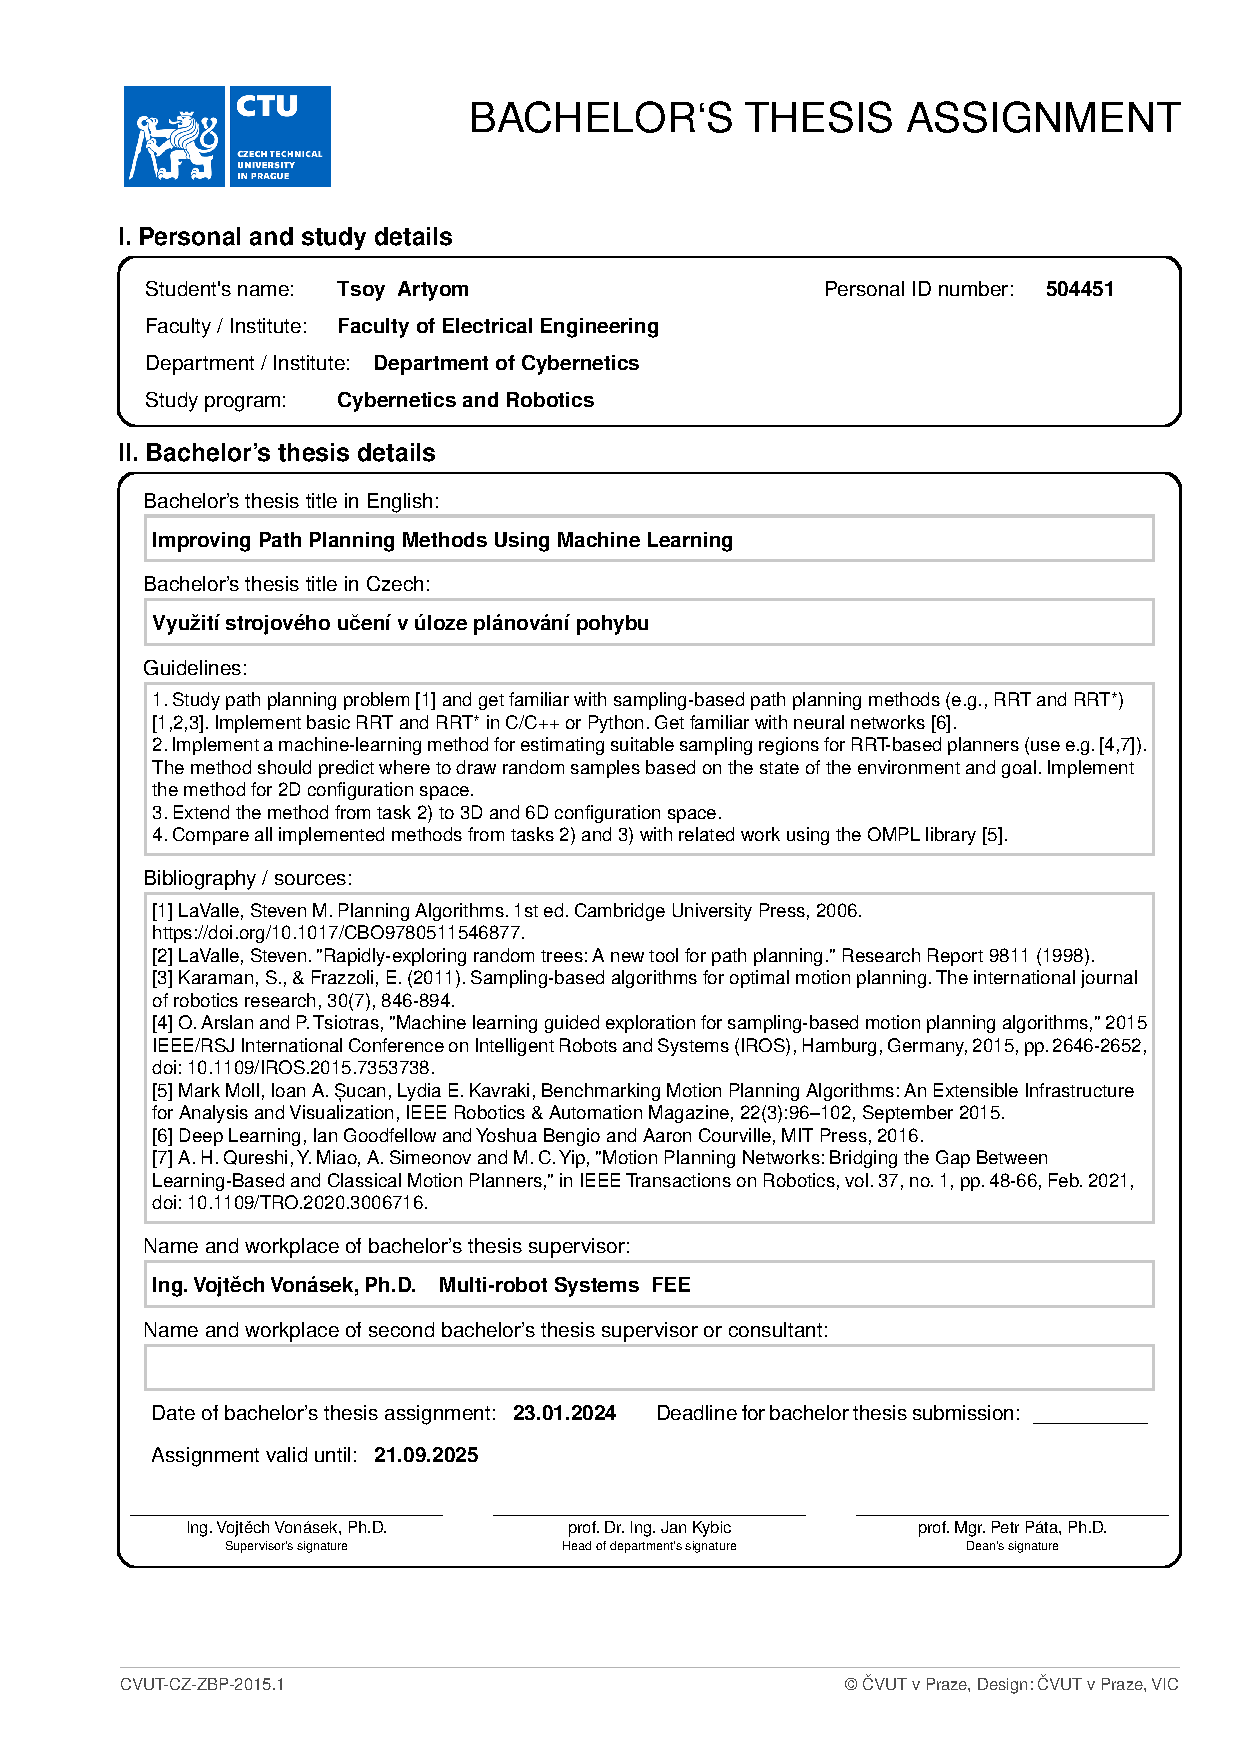
\includepdf[pages=1]{BP.pdf}
\includepdf[pages=2]{BP.pdf} 
%---------------------------------------------------------------------------------
\chapter{Introduction}
\label{chap:Introduction}
Path planning is a fundamental challenge in the field of robotics, 
essential for enabling autonomous systems to navigate through complex environments efficiently. 
It allows vehicles or robots to find the shortest, 
obstacle-free route from their starting point to their destination.
This route, often represented as a series of states comprising position and orientation or as waypoints, 
guides the vehicle or robot towards its goal effectively. 
One of the famous examples is the Piano Movers Problem.
Path planning involves determining the optimal route or path for transporting a 
piano from one location to another while navigating through various obstacles and constraints. 
In Figure \ref{fig:piano}, the illustration of the Piano Movers Problem is depicted.\\[12pt]
%------
Traditional path planning methods, such as Rapidly-exploring Random Trees (RRT)~\cite{lavalle1998rapidly} 
and its enhanced variant RRT*~\cite{karaman2011rrtstar}, 
have been widely used due to their effectiveness in handling high-dimensional configuration spaces.  
The configuration space, often denoted as $\mathcal{C}$-space, is a fundamental concept in robotics and motion planning. 
It represents all possible configurations or states that a robot or system can occupy within its environment.\\[12pt]
%------
To enhance clarity within the text, it is crucial to briefly explain how RRT works: 
The algorithm incrementally builds a tree structure from an initial configuration towards randomly sampled configurations in the configuration space.
At each iteration, a new configuration, known as a random sample, is generated within the configuration space. 
The algorithm then extends the existing tree towards this random sample by selecting the nearest node (configuration) in the tree to the sample and moving towards it in small increments.
The key idea behind RRT is to rapidly explore the configuration space by growing the tree towards unexplored regions. 
This exploration strategy ensures that the algorithm efficiently covers the space while avoiding costly computation.
RRT continues this process iteratively, gradually expanding the tree towards the goal configuration. 
As the algorithm progresses, the tree becomes denser in regions that are closer to the goal, eventually converging to a path from the start to the goal configuration.
In Figure \ref{fig:RRTsimple}, simple examples of how RRT looks can be seen.\\[12pt]
%------
However, with the increasing complexity of real-world environments, 
such as systems with many obstacles or narrow passages, as illustrated in Figure \ref{fig:narrowpassage},
there is a growing need to enhance these methods to improve their efficiency and
adaptability.
Efficiency in path planning denotes the capability of the algorithms to generate feasible paths within a reasonable timeframe, 
while adaptability refers to its ability to dynamically adjust strategies in response to changes in environmental conditions or task requirements.
%---------------------------------------------------------------------------------
% \begin{figure}
%   \centering
%   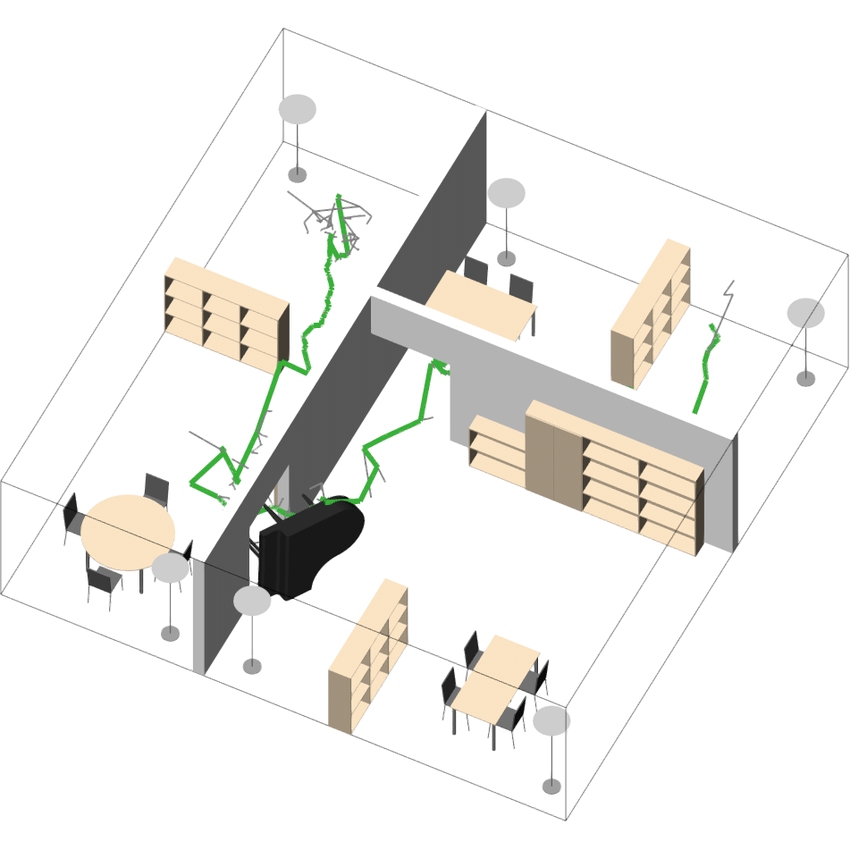
\includegraphics[width=0.5\linewidth]{figChap1/The-piano-movers-problem-EET.png}
%   \caption{The Piano Movers Problem \cite{rickert2014piano}.} 
%   \label{fig:piano}
% \end{figure}
 
% \begin{figure} 
%   \centering 
%   \begin{minipage}[t]{1\textwidth}
%       \centering
%       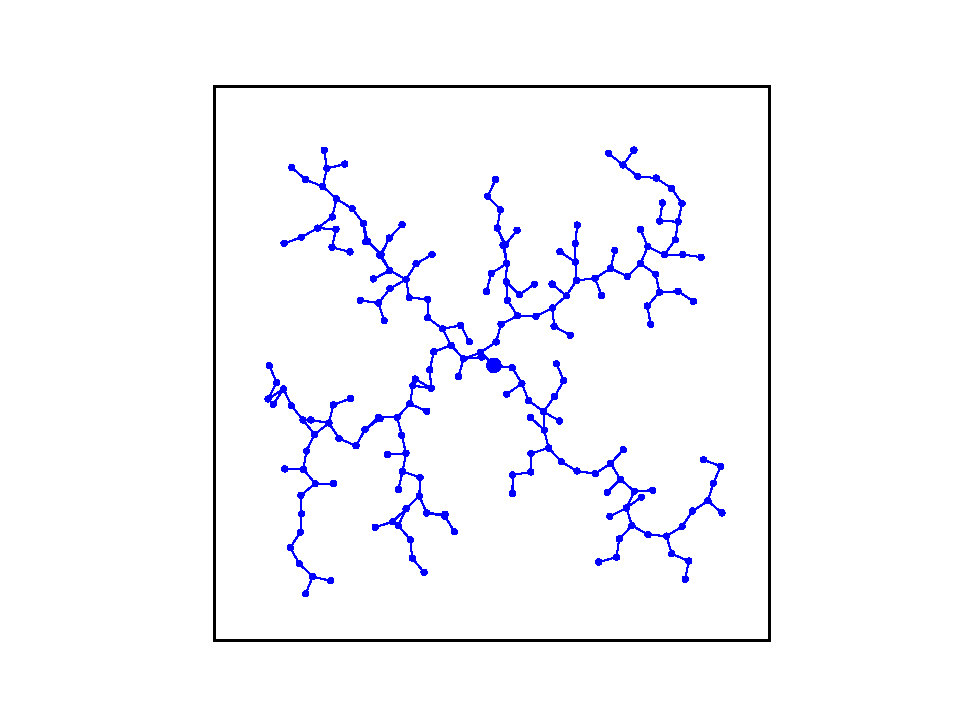
\includegraphics[width=0.7\textwidth]{figChap1/RRTsimple2.pdf} 
%   \end{minipage} 
%   \caption{Rapidly-exploring Random Trees examples.} 
%   \label{fig:RRTsimple}
% \end{figure}

\begin{figure}
  \centering
  \begin{subfigure}[b]{0.4\textwidth}
      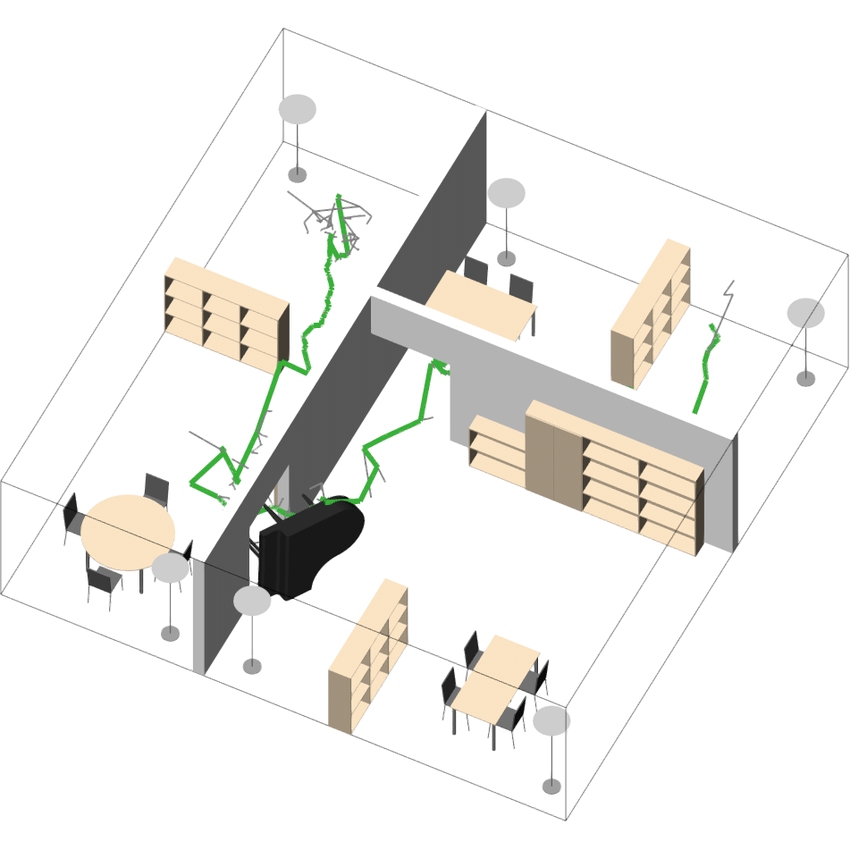
\includegraphics[width=\textwidth]{figChap1/The-piano-movers-problem-EET.png}
      \caption{The Piano Movers Problem. Image courtesy of~\cite{rickert2014piano}.}
      \label{fig:piano}
  \end{subfigure}
  ~ %add desired spacing between images, e. g. ~, \quad, \qquad, \hfill etc. 
    %(or a blank line to force the subfigure onto a new line)
  \begin{subfigure}[b]{0.5\textwidth}
      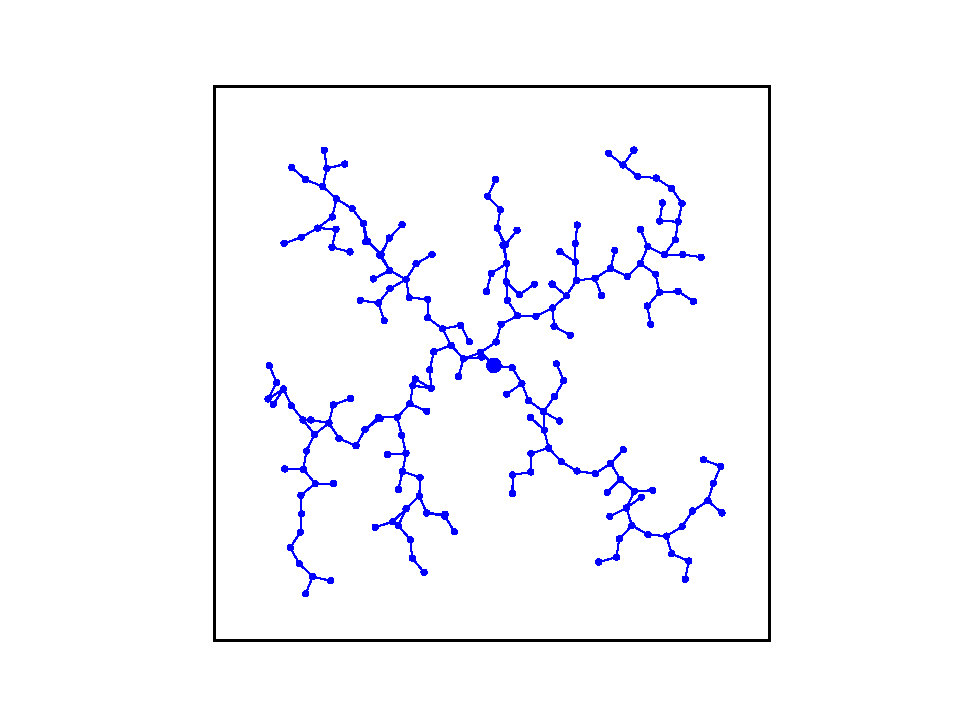
\includegraphics[width=\textwidth]{figChap1/RRTsimple2.pdf}
      \caption{Rapidly-exploring Random Trees examples.}
      \label{fig:RRTsimple}
  \end{subfigure} 
  \caption{Figure \ref{fig:piano} illustrates an example of a path planning problem, 
  along with a representation of the Rapidly-exploring Random Tree (RRT) algorithm in Figure \ref{fig:RRTsimple}.}%\label{fig:animals}
\end{figure}


\begin{figure} 
  \centering 
  \begin{minipage}[t]{0.9\textwidth}
      \centering
      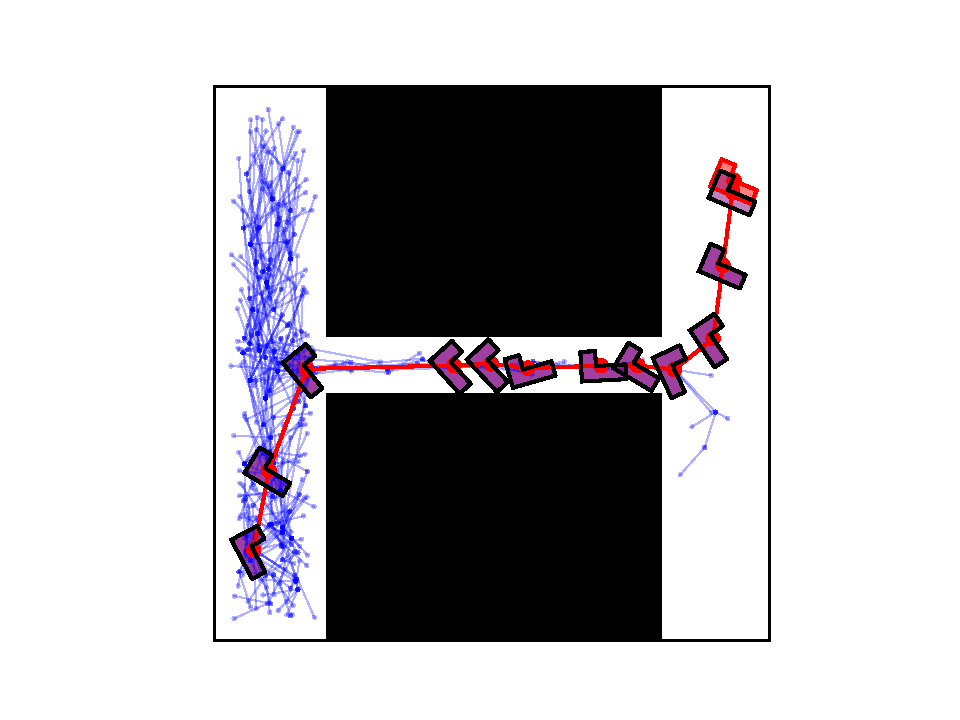
\includegraphics[width=0.9\textwidth]{figChap1/narrow_passage.pdf} 
  \end{minipage} 
  \caption{Illustration of the narrow passage where the aim is to maneuver a purple object through the limited space between black obstacles to reach the red goal configuration.} 
  \label{fig:narrowpassage}
\end{figure}

%---------------------------------------------------------------------------------
%---------------------------------------------------------------------------------
\section{Machine Learning}

Understanding the concept of machine learning is pivotal for comprehending 
its utilization within this thesis. 
Therefore, this section will offer a brief explanation of machine learning without 
delving into mathematical definitions and complex explanations.
Main idea and inspiration for this section is drawn from~\cite{Goodfellow-et-al-2016DeepLearning}.\\[12pt]
%------
Machine learning is a field of artificial intelligence that focuses on developing algorithms 
capable of learning patterns and making predictions from data without being explicitly programmed. 
It enables computers to learn from past experiences and improve their performance over time.\\[12pt]
%------
Most machine learning algorithms can be categorized into supervised learning and unsupervised learning. 
In supervised learning, the algorithm receives guidance from an instructor or teacher, 
who provides the target output for each input example. 
Conversely, unsupervised learning involves no external guidance, 
requiring the algorithm to derive insights from the data independently.\\[12pt]
%------
Supervised learning tasks typically include classification, regression, 
and density estimation or probability mass function estimation. 
In classification tasks, the algorithm classifies input data into predefined categories or classes. 
For instance, object recognition can be considered a classification task, 
where the computer program identifies objects in images and assigns them to specific categories.
In Figure \ref{fig:ObjectDetection}, an example of object recognition is depicted.\\[12pt]
%------
In regression tasks, the algorithm predicts a numerical value based on input data. 
For example, predicting house prices based on features like location, 
size, and amenities is a regression task.\\[12pt]
%------
Density estimation involves learning a function $p_{\text{model}}: \mathbb{R}^n \rightarrow \mathbb{R}$, 
where $p_{\text{model}}(x)$ represents a probability density function for continuous data or a probability mass function for discrete data. 
The algorithm learns the underlying data structure, 
identifying regions where examples are densely clustered and areas where they are less likely to occur. 
This understanding is crucial for effectively modeling the data distribution.\\[12pt]
%------
This thesis aims to improve path planning algorithms by using machine learning, 
including classification and density estimation techniques.

%---------------------------------------------------------------------------------
\begin{figure}
  \centering
  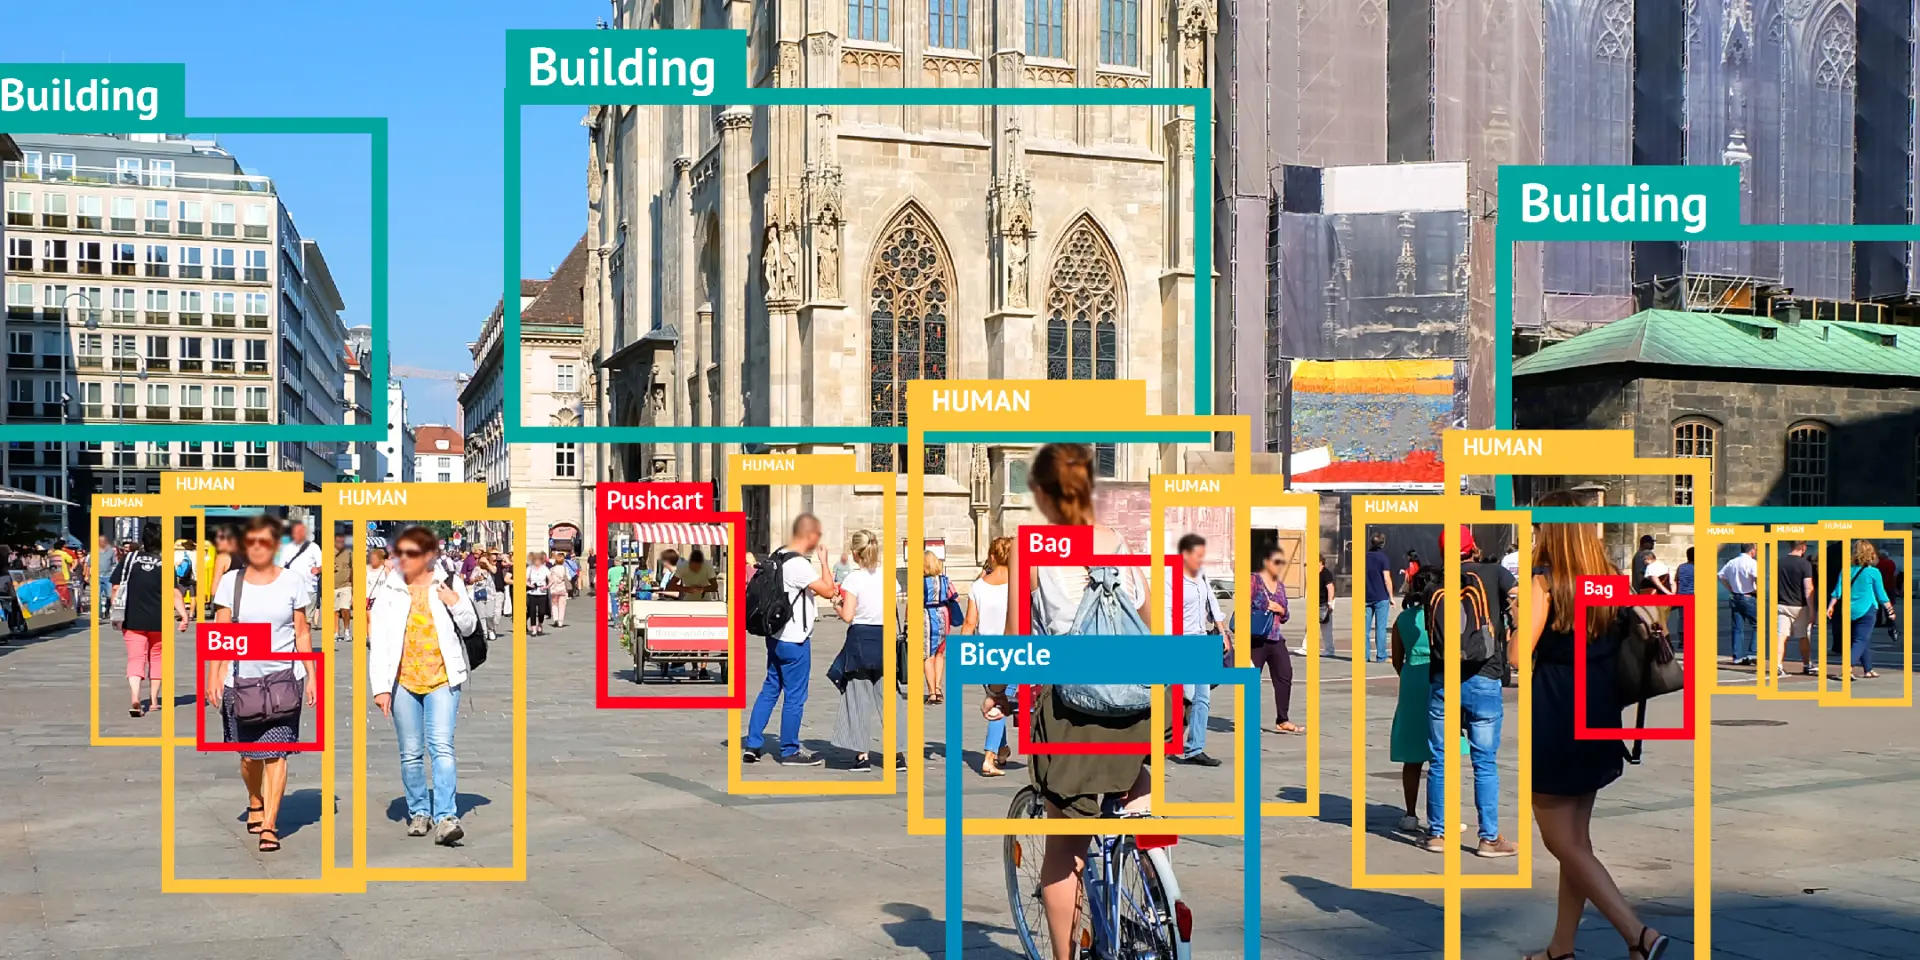
\includegraphics[width=1\linewidth]{figChap1/Object_detection.pdf}
  \caption{An example of an object classification problem, 
  where the program classifies objects in the photo into their respective classes.
  Image courtesy of~\cite{ObjectDetection}.}
  \label{fig:ObjectDetection}
\end{figure} 
 
%---------------------------------------------------------------------------------
%---------------------------------------------------------------------------------
\section{Thesis structure}

% The primary objective of this thesis is to develop and implement machine learning-based approaches to improve the performance of sampling-based path planning methods. 
% By integrating machine learning methods into the path planning process, 
% we seek to enhance the ability of the algorithms to adapt to varying environmental conditions and goals.
% \\\\
Chapter \ref{chap:Introduction} introduces the concepts of path planning and machine learning. 
It outlines the central objectives of this thesis, focusing on the integration of machine learning techniques to enhance path planning algorithms. 
Additionally, Chapter \ref{chap:Introduction} provides a concise overview of the thesis structure.\\[12pt]
%------
Chapter \ref{chap:Task formulation} will delve deeper into the path planning problem, 
offering an understanding of essential terms and notations. 
Building on this foundation, the Chapter \ref{chap:Task formulation} will formulate the challenge of this thesis.\\[12pt]
%------
In Chapter \ref{chap:RelatedWorks}, familiarity with sampling-based methods, including RRT and RRT*, will be gained.\\[12pt]
%------
Chapter \ref{chap:Improving RRT*} will be pivotal, 
as it will explain the machine learning methods employed in this study. 
Additionally, it will detail the integration of these methods into the sampling-based algorithm RRT* in both 2D $\mathcal{C}$-space and its extension to 3D $\mathcal{C}$-space.\\[12pt]
%------
The effectiveness of the developed methods will be evaluated in Chapter \ref{chap:Result} through comparisons with existing algorithms 
using the Open Motion Planning Library (OMPL)~\cite{Ioan2012ompl}.\\[12pt]
%------
In Chapter \ref{chap:Conclusion}, the thesis will be concluded by summarizing all results and findings.

%---------------------------------------------------------------------------------
%---------------------------------------------------------------------------------
%---------------------------------------------------------------------------------
\chapter{Task formulation}   
\label{chap:Task formulation}

This chapter lays the foundation for better understanding the research objectives and motivations.
Firstly, it will explain the path planning problem and provide a brief introduction to sampling-based path planning, 
including an overview of its definition, advantages, and disadvantages. 
Based on this, the main objective of the thesis is formulated. 
Subsequently, key terms related to path planning are elucidated to ensure clarity and comprehension. 
Finally, the chapter concludes by formulating the primary challenge addressed in the thesis.
%---------------------------------------------------------------------------------
%---------------------------------------------------------------------------------
\section{Path planning problem}
% \textbf{u need to understand differnce btw path planning and motion planning. 
% Here also u can add an example of piano mevers problem with better explanation.
% In itroduction part u just briefly metioned about that. Here u can write more.
% Reader will better understand text if u provide a simple and good explained exaple :)
% use definition of motion planning from \cite{Moll2015BenchmarkingMotionPlanningAlgos}}
% \\\\
The path planning problem, also known as motion planning or the navigation problem, 
is a fundamental challenge in robotics. 
It involves finding a path that connects a start configuration to a goal configuration while 
satisfying specified constraints, such as avoiding collisions.\\[12pt]
%------
The path planning problem and relevant terms will be explained using the Piano Movers Problem.
An illustration of this problem can be seen in Figure \ref{fig:piano}. 
In this scenario, the task is to move a piano from one room to another trying 
not to collide with any objects.\\[12pt]
%------
The piano has six degrees of freedom (DoF), 
meaning its position in space can be described using six coordinates: three for position ($x, y, z$) 
and three for rotation ($yaw, roll, pitch$). 
The position most often represents the coordinates of its center of mass or as a reference point of the robot.
It can be stated that there a \textbf{6D $\mathcal{C}$-space} because to describe the configuration of the piano, we need six coordinates.
These coordinates define configurations of the piano.\\[12pt]
%------
Our objective is to find a sequence of configurations that safely moves the piano 
from its starting position to its destination without colliding with any objects in the room.
Objects like tables, closets, walls represent \textbf{obstacles}, and the door represents \textbf{narrow passage}. 
These obstacles must be avoided. 
To avoid these obstacles, a sequence of configurations is sought. 
This sequence is referred to as a \textbf{path}. 
The problem of path planning can be stated as finding a collision-free path 
from the initial point to the goal point.
%---------------------------------------------------------------------------------
%---------------------------------------------------------------------------------
\section{Sampling-based path planning}
% \textbf{Put here sentences form Research objectives and in research objectives left only advanteges and disadvantages 
% of sampling based planers. according on this u will formulate the main objective of research :)}
% \\\\ 
Sampling-based path planning~\cite{Lavalle2006PlanningAlgos} is a computational approach utilized in robotics to generate feasible paths for autonomous agents navigating through complex environments. 
One of the sampling-based algorithms is the Rapidly-exploring Random Tree (RRT)~\cite{lavalle1998rapidly}.\\[12pt]
%------
Unlike traditional grid-based methods such as A*~\cite{Hart1968Astar}, 
which discretize the environment into a grid and search for paths within this grid, as illustrated in Figure \ref{fig:Astargrid}, 
sampling-based methods operate by randomly sampling points in the configuration space.
In the case of the Piano Movers Problem, a random sample represents random values for ($x, y, z, yaw, roll, pitch$).
Subsequently, these sampled points are used to construct a graph.
This probabilistic approach allows for efficient exploration of high-dimensional spaces and is particularly well-suited for environments with complex obstacles.\\[12pt]
%------
The main goal of sampling-based algorithms in path planning is to efficiently explore the configuration space to find feasible paths from a start configuration to a goal configuration, 
while avoiding obstacles.
%---------------------------------------------------------------------------------
%---------------------------------------------------------------------------------
\section{Research Objectives} 
Sampling-based algorithms offer several advantages. 
They are flexible and can handle high-dimensional configuration spaces, 
making them suitable for complex environments with obstacles and constraints. 
Additionally, they are computationally efficient, 
focusing on sampling feasible configurations rather than exhaustive exploration.\\[12pt]
%------
However, sampling-based methods also have their disadvantages. 
Random sampling can create biases in certain areas of the configuration space, 
resulting in less-than-optimal paths or missing potential solutions.
In highly cluttered environments or spaces with narrow passages, 
these algorithms may struggle to adequately explore the configuration space, 
resulting in incomplete coverage and suboptimal path generation. 
It can be seen in Figure \ref{fig:narrowpassage2}.
The performance of sampling-based algorithms can be sensitive to various parameters, 
such as sampling density and collision checking threshold. 
Additionally, while they offer computational efficiency, 
they may not always generate the highest quality paths compared to other methods, 
especially in scenarios where path smoothness or optimality is crucial.\\[12pt]
%------
The research objectives of this thesis will concentrate on enhancing 
sampling-based algorithms by addressing their limitations in scenarios characterized by 
numerous obstacles or narrow passages. 
The primary goal is to enhance sampling-based algorithms through the integration of machine learning techniques to 
more effectively generate points. 
The proposed approach will improve random sampling by selectively sampling points 
only from obstacle-free spaces, 
thereby enhancing the efficiency and adaptability of the algorithms.
%---------------------------------------------------------------------------------
% \begin{figure}
%   \centering
%   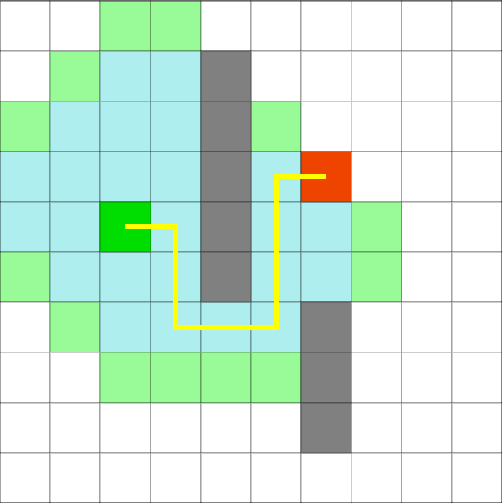
\includegraphics[width=0.4\linewidth]{figChap2/A-star-on-grid-map.png}
%   \caption{A-star algorithm realizes path-finding on grid map.
%   Image courtesy of \cite{Xie2022Astarfoto}.}
%   \label{fig:Astargrid}
% \end{figure} 

% \begin{figure} 
%   \centering 
%   \begin{minipage}[t]{1\textwidth}
%       \centering
%       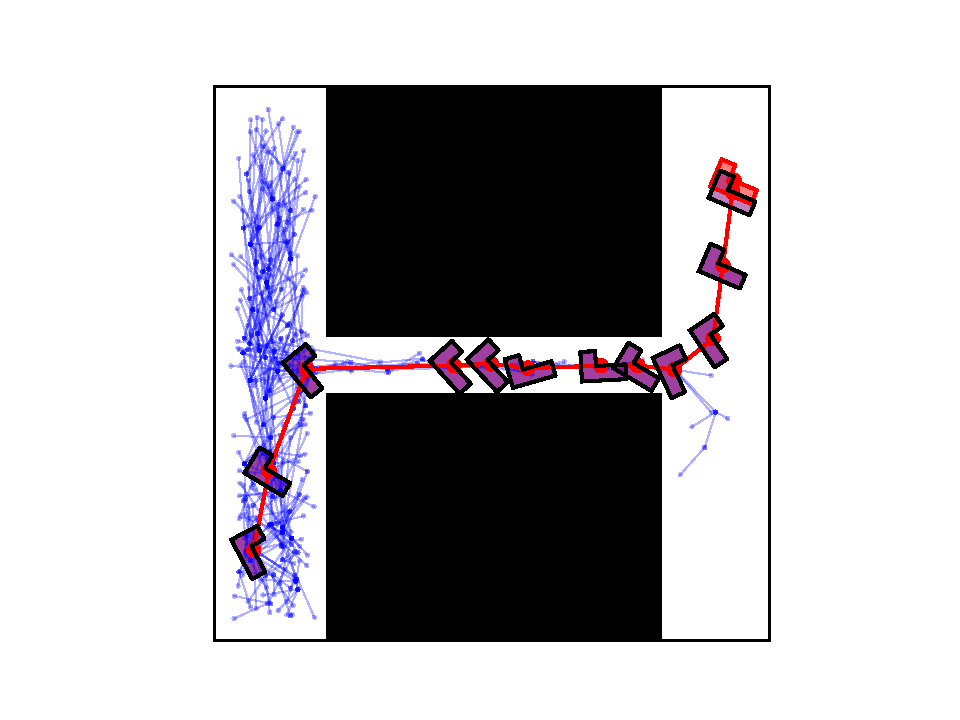
\includegraphics[width=0.9\textwidth]{figChap1/narrow_passage.pdf} 
%   \end{minipage} 
%   \caption{Illustration of the narrow passage, 
%   where the blue lines represent RRT* exploration in configuration space.
%   It can be seen that numerous samples were generated on the left side, 
%   resulting in incomplete coverage of the space. 
%   In summary, a large number of samples were generated in inappropriate locations.} 
%   \label{fig:narrowpassage2}
% \end{figure} 


\begin{figure}
  \centering
  \begin{subfigure}[b]{0.36\textwidth}
      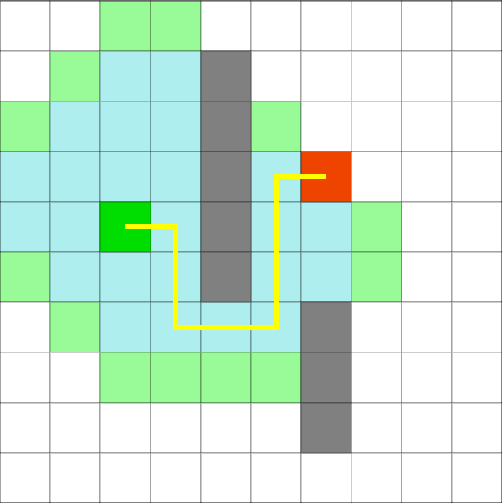
\includegraphics[width=\textwidth]{figChap2/A-star-on-grid-map.png}
      \caption{A* algorithm.
        Image courtesy of~\cite{Xie2022Astarfoto}.}
      \label{fig:Astargrid}
  \end{subfigure}
  ~ %add desired spacing between images, e. g. ~, \quad, \qquad, \hfill etc. 
    %(or a blank line to force the subfigure onto a new line)
  \begin{subfigure}[b]{0.61\textwidth}
      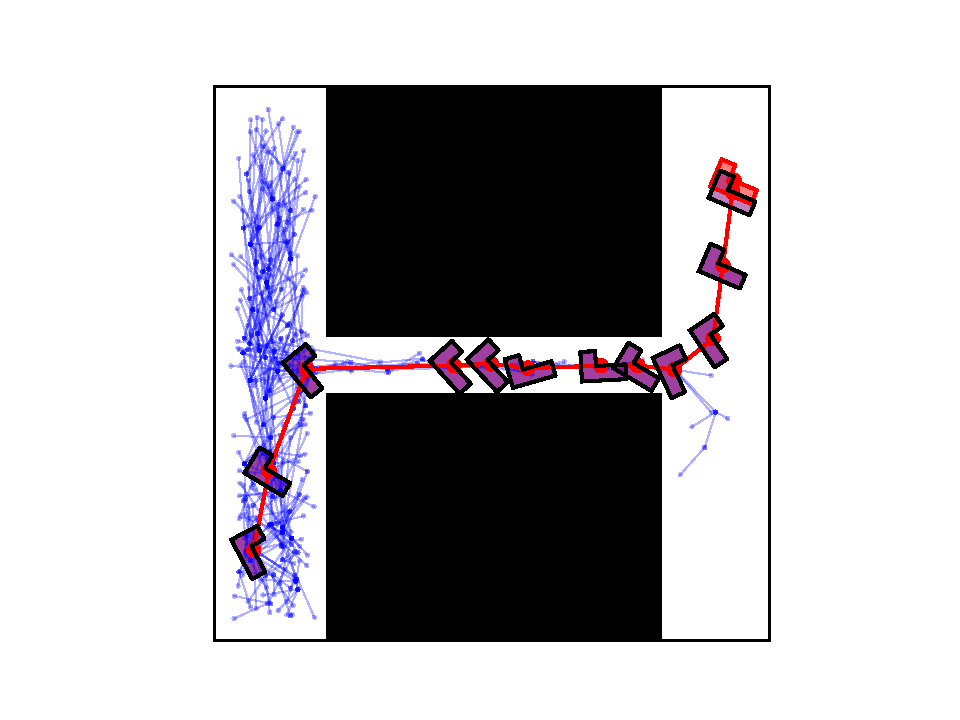
\includegraphics[width=\textwidth]{figChap1/narrow_passage.pdf}
      \caption{Narrow passage in 3D $\mathcal{C}$-space.}
      \label{fig:narrowpassage2}
  \end{subfigure} 
  \caption{llustration of the A-satr algorithm realizes path-finding on grid map in Figure \ref{fig:Astargrid} and 
  illustration of the narrow passage in Figure \ref{fig:narrowpassage2}, 
  where the blue lines represent RRT* exploration in configuration space.
  It can be seen in Figure \ref{fig:narrowpassage2} that numerous samples were generated on the left side, 
  resulting in incomplete coverage of the space. 
  In summary, a large number of samples were generated in inappropriate locations.} 
\end{figure}

%---------------------------------------------------------------------------------
%---------------------------------------------------------------------------------
\section{Components of the Path Planning Problem}

Let us begin by defining the configuration space, denoted as $\mathcal{C}$. 
It serves as a critical component of motion planning, representing all possible states of system. 
This space is a subset of $\mathbb{R}^d$, where $d \geq 2$ and $d \in \mathbb{N}$. 
Within $\mathcal{C}$, there are three primary regions:

\begin{itemize}
    \item \textbf{Obstacle Space ($\mathcal{C}_{\text{obs}}$):} This region encompasses areas occupied by obstacles, constraining the motion of our system.
    \item \textbf{Obstacle-Free Space ($\mathcal{C}_{\text{free}}$):} Defined as the complement of $\mathcal{C}_{\text{obs}}$ within $\mathcal{C}$, this space allows unrestricted movement for our system.
    \item \textbf{Goal Region ($\mathcal{C}_{\text{goal}}$):} Representing the destination our system aims to reach. 
    This region must be within the free space $\mathcal{C}_{\text{goal}} \subseteq \mathcal{C}_{\text{free}}$, 
    as the system cannot reach regions outside of the free space. 
    Within this region, 
    there must exist a goal configuration, 
    denoted as $q_{\text{goal}}\in \mathcal{C}_{\text{goal}}$, 
    which represents the optimal configuration.
    However, it is notable that in certain cases, 
    the goal region may be represented just by $q_{\text{goal}}$.
\end{itemize} 
Path planning aim to find a feasible path from the initial configuration $q_{\text{start}} \in \mathcal{C}_{\text{free}}$ 
to a goal configuration $q_{\text{goal}} \in \mathcal{C}_{\text{goal}}$, 
ensuring avoidance of regions occupied by obstacles ($\mathcal{C}_{\text{obs}}$).\\[12pt]
%------
To represent the connectivity between configurations within $\mathcal{C}_{\text{free}}$, a graph $G = (V, E)$ is utilized. 
Here, $V$ denotes the finite set of vertices, each corresponding to a configuration point, 
and $E \subseteq V \times V$ denotes the set of edges, signifying connections between configurations.\\[12pt]
%------
In Figure \ref{fig:config_space}, a simple 2D $\mathcal{C}$-space is depicted. 
The start configuration, denoted by $q_{\text{start}}$, is marked in green, 
while the goal configuration, denoted by $q_{\text{goal}}$, is marked in red. 
The black circle at the center of the space represents an obstacle. 
The blue trajectory, comprising vertices and edges, 
illustrates the path through the configuration space. 
These vertices, represented as blue circles, illustrates configurations or nodes along the path.

%---------------------------------------------------------------------------------
\begin{figure}
  \centering
  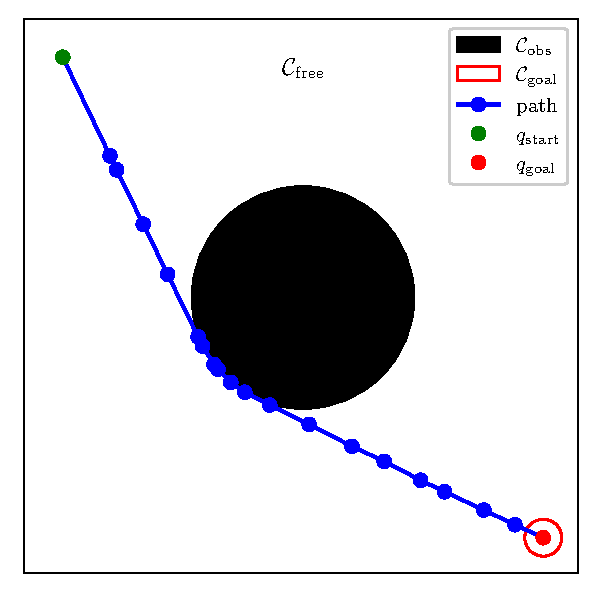
\includegraphics[width=0.6\linewidth]{figChap2/ConfigSpace.eps}
  \caption{2D $\mathcal{C}$-space.}
  \label{fig:config_space} 
\end{figure} 
%---------------------------------------------------------------------------------
%---------------------------------------------------------------------------------
\section{The Challenge}

% The primary focus lies in improving the RRT* algorithm, 
% which employs random sampling points to construct a graph representing feasible paths.  
The challenge of this thesis is to reduce the number of 
sampling points, or iterations, 
required to converge on the optimal path. 
This will be achieved by learning 
the configuration space and generating points within $\mathcal{C}_{\text{free}}$ 
and enhance the overall efficiency of the motion planning algorithm. 
Further information is provided in Chapter \ref{chap:Improving RRT*}.
 
%---------------------------------------------------------------------------------
%---------------------------------------------------------------------------------
%---------------------------------------------------------------------------------
\chapter{Related works} 
\label{chap:RelatedWorks}
% \textbf{Add here RRT, RRT star, PRM, RRT sharp, Informed RRT star LazyRRT, TRRT. 
% Focus on algorithms where u find good explanations of them. Also bcz we are talking about ML and 
% u have this as a bibliography source, add information about Motion Planning Networks \cite{Ahmed2019MotionPlanningNetworks}
% Delete chapters about comparison RRT and RRT*, add this information to RRT* chapter and talk about his advantages
% according to this show your examples in 2D and 6D Configguration Space. U can not talk about 3D Configuration Space, 
% because u will show it in Chapter 4, where u will show enchance version of RRT star in 3D conf space. add new fotos of 6D cnof space 
% in pdf format. You need also to describe how we found a path in RRT (explain Retrace function, just some sentences
% that every point has only one parent blah blah blah and when we found goal we just strat finding parent of parent of parent etc..
% maybe add some figure for this. but honestly this chapter has too many figures, try to left only relevant or maybe generate figure
% where will be two features instead of one in two figures. Try to fully explain main idea for reader who nows nothing.
% Explain RRT star, this is a hard algorithm which one u implement, u can )}
% \\\\
In this chapter, an overview of various path planning methods will be presented. 
This exploration is crucial for gaining a deeper understanding of how 
sampling algorithms function and how they can be enhanced. 
Building upon this understanding, 
the main idea of improvement was implemented, 
and the foundation for this implementation was laid upon the knowledge of 
sampling-based algorithms. 
These methods will be described and analyzed to provide 
insights into their effectiveness and limitations.
%---------------------------------------------------------------------------------
%---------------------------------------------------------------------------------
\section{Rapidly-exploring Random Tree (RRT)} 
The Rapidly-exploring Random Tree (RRT)~\cite{lavalle1998rapidly} algorithm 
is a versatile and widely used sampling-based motion planning algorithm in robotics. 
A pseudocode is shown in Algorithm \hyperref[alg:rrt]{\ref*{alg:rrt}}.
Its appeal lies in its efficiency in exploring high-dimensional configuration spaces, 
making it suitable for various robotic applications. 
RRT excels in systems with non-holonomic constraints, 
which limit a robot's movement beyond just its position and orientation. 
These constraints often involve restrictions on how the robot can change its velocity or direction. 
In the Fig. \hyperref[fig:RRTgrowing]{\ref*{fig:RRTgrowing}}, 
the progressive expansion in 2D $\mathcal{C}$-space of the RRT can be seen.
%---------------------------------------------------------------------------------
\begin{figure}[!ht]
  \centering
  \begin{subfigure}[b]{0.3\textwidth}
      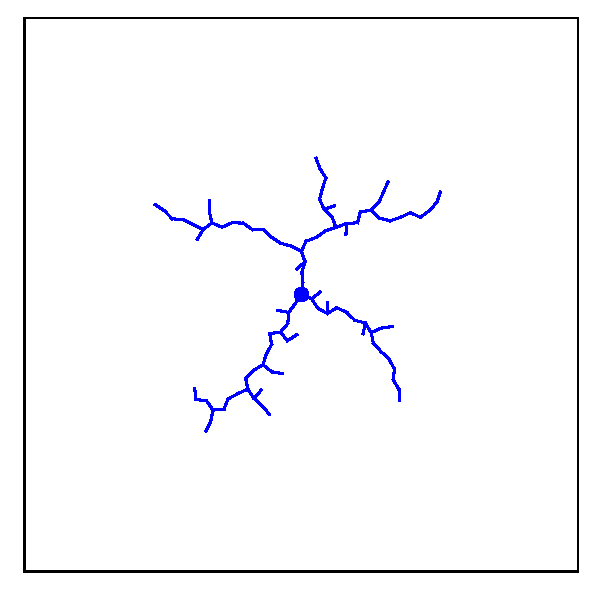
\includegraphics[width=\textwidth]{figChap3/2RRTexpansion100.eps}
      \caption{100 iterations}
      % \label{fig:gull}
  \end{subfigure}
  ~ %add desired spacing between images, e. g. ~, \quad, \qquad, \hfill etc. 
    %(or a blank line to force the subfigure onto a new line)
  \begin{subfigure}[b]{0.3\textwidth}
      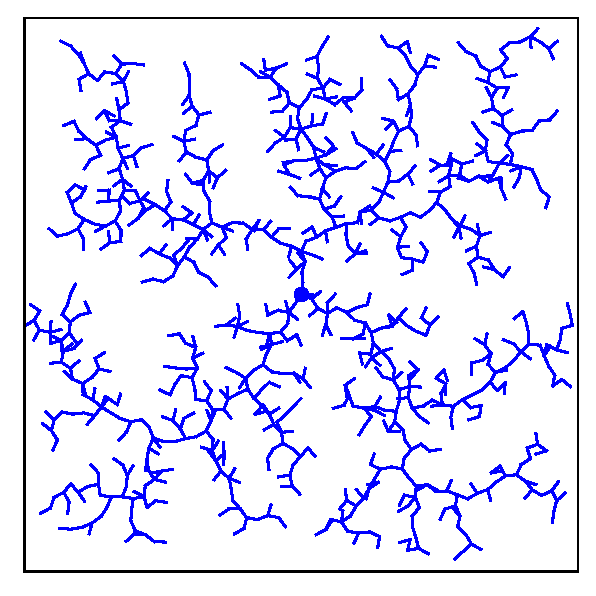
\includegraphics[width=\textwidth]{figChap3/2RRTexpansion1000.eps}
      \caption{1000 iterations}
      % \label{fig:tiger}
  \end{subfigure}
  ~ %add desired spacing between images, e. g. ~, \quad, \qquad, \hfill etc. 
  %(or a blank line to force the subfigure onto a new line)
  \begin{subfigure}[b]{0.3\textwidth}
      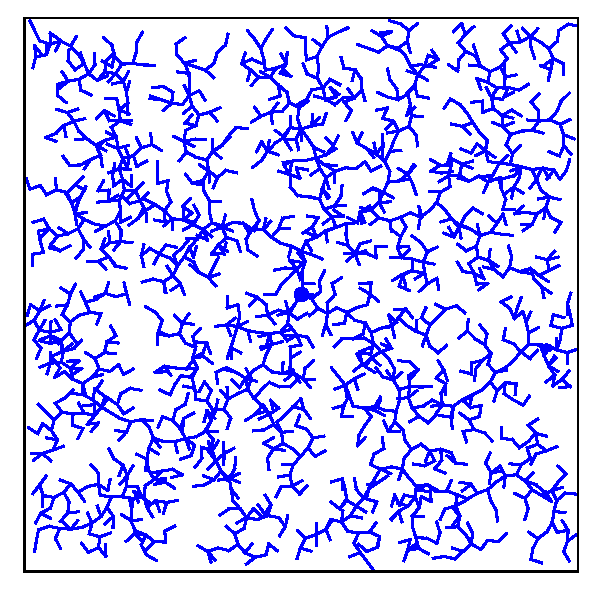
\includegraphics[width=\textwidth]{figChap3/2RRTexpansion2000.eps}
      \caption{2000 iterations}
      % \label{fig:mouse}
  \end{subfigure}
  \caption{Example of RRT expansion in 2D $\mathcal{C}$-space.}
  \label{fig:RRTgrowing}
\end{figure} 
%---------------------------------------------------------------------------------
\\
Simplicity and effectiveness of the RRT algorithm have made it a popular choice among researchers and practitioners in the field.
This highlights the importance of explainig its operational phases.\\[12pt]
%------
In the initialization phase, 
the algorithm begins by establishing a tree structure with only the initial state, 
which represents the root node. 
This initial state represents the starting configuration of the robot or system.\\[12pt]
%------
During the expansion phase, 
the algorithm iteratively executes the following steps until a predetermined number of iterations 
or the goal state is reached: generating a random state within the configuration space, 
identifying the nearest node in the existing tree to the randomly generated state, 
extending the tree towards the random state by incrementally advancing in its direction 
and creating a new node, 
and subsequently verifying whether the new node collides with any obstacles. 
If no collision occurs, 
the new node is added to the tree, thereby expanding the coverage of the configuration space.\\[12pt]
%------
After completion of each iteration, 
the algorithm conducts goal checking to determine if the goal state has been reached. 
Upon reaching the goal state, 
the algorithm terminates, 
and the path to the goal is extracted from the tree structure.\\[12pt]
%------
To extract a path to the goal, a hierarchical structure within the tree must be established. 
For every configuration added into the tree, 
a parent configuration is assigned, typically being the nearest configuration in the tree. 
This parent configuration acts as the reference point from which 
the new configuration is generated or ``steered'' towards. 
Consequently, each configuration has only one parent but can have many children, 
thereby forming a hierarchical relationship within the tree.
%---------------------------------------------------------------------------------
\begin{figure}[!ht]
  \centering
  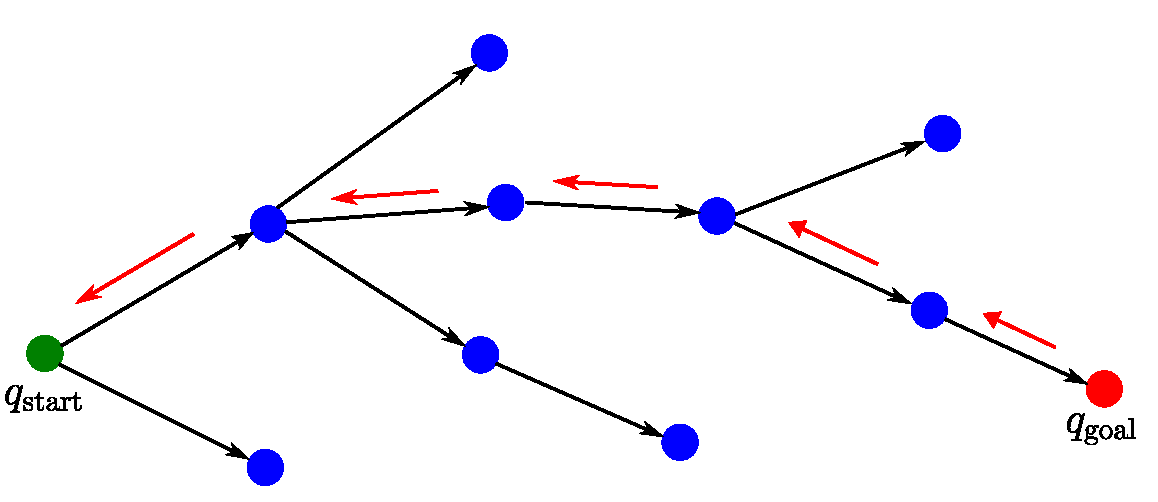
\includegraphics[width=0.8\linewidth]{figChap3/ParentChild4.pdf}
  \caption{An illustration of a hierarchical structure, 
  where black arrows indicate the parent-child relationships, 
  with the origin of the arrow representing a parent node and 
  its destination denoting a child node. 
  Additionally, red arrows illustrate a retracing process, 
  indicating the movement from the goal configuration back to 
  the start configuration by moving through parent nodes.}
  \label{fig:ParentChild}
\end{figure} 
%---------------------------------------------------------------------------------
\\
Upon reaching the goal configuration, 
the path to the start configuration is retraced by traversing from the goal configuration 
to its parent and then recursively traversing through each parent until 
the start configuration is reached. 
In Figure \ref{fig:ParentChild}, an illustration of this process is presented.
This process capitalizes on the parent-child relationships established during 
the tree construction phase, 
enabling systematic navigation from the goal configuration back to the start configuration, 
and thereby facilitating path extraction.\\[12pt]
%------
The RRT algorithm is known for its relatively straightforward implementation, 
yet it effectively explores the configuration space. 
This efficiency refers to its ability to rapidly expand the search space, 
thereby quickly accessing various regions of the configuration space. 
However, despite these advantages, RRTs are not without their limitations. 
One notable drawback is their tendency towards suboptimality. 
Unlike certain other algorithms, basic RRTs do not guarantee the discovery of the optimal path to the goal. 
Consequently, the path found may not be the shortest or most efficient route. 
Furthermore, RRTs often necessitate frequent collision checks, 
particularly in environments characterized by clutter, 
leading to a notable increase in computational time.\\[12pt]
%---------------------------------------------------------------------------------
\begin{algorithm}[H]
  \caption{Rapidly-exploring Random Tree (RRT)}
  \label{alg:rrt} 
  \KwData{Start configuration $q_{\text{start}}$, Number of iterations $K$}
  \KwResult{RRT tree $T$}
  \vspace{0.1cm}
  \hrule
  \vspace{0.2cm}
  Initialize tree $T$ with root $q_{\text{start}}$\;
  \For{$k \gets 1$ \KwTo $K$}{
    Generate random configuration $q_{\text{rand}} \in \mathcal{C}$\;
    Find nearest node $q_{\text{near}}$ in $T$ to $q_{\text{rand}}$\;
    Steer towards $q_{\text{rand}}$ to get new node $q_{\text{new}}$\;
    
    \If{ObstacleFree($q_{\text{near}}$, $q_{\text{new}}$)}{
      Add $q_{\text{new}}$ to $T$ with an edge from $q_{\text{near}}$\;
      \If{GoalFound($q_{\text{new}}$)}{
      \textbf{break}\;
      }
    }
  }
  
  \Return $T$\;
\end{algorithm}
 

%---------------------------------------------------------------------------------
%---------------------------------------------------------------------------------
%---------------------------------------------------------------------------------
\section{Rapidly-exploring Random Tree star (RRT*)}
 
The Rapidly-exploring Random Tree Star (RRT*)~\cite{karaman2011rrtstar} also known as 
Optimal RRT is an extension of the original RRT algorithm 
designed to enhance the efficiency and optimality of path planning in robotics.
A pseudocode is shown in Algorithm \hyperref[alg:rrt_star]{\ref*{alg:rrt_star}}. 
%---------------------------------------------------------------------------------
\begin{figure}[!ht]
  \centering
  \begin{subfigure}[b]{0.3\textwidth}
      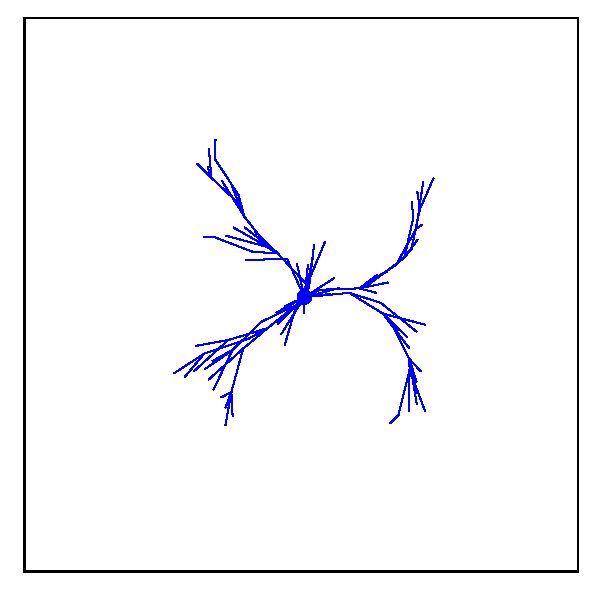
\includegraphics[width=\textwidth]{figChap3/RRTstar_expansion100.eps}
      \caption{100 iterations}
      % \label{fig:gull}
  \end{subfigure}
  ~ %add desired spacing between images, e. g. ~, \quad, \qquad, \hfill etc. 
    %(or a blank line to force the subfigure onto a new line)
  \begin{subfigure}[b]{0.3\textwidth}
      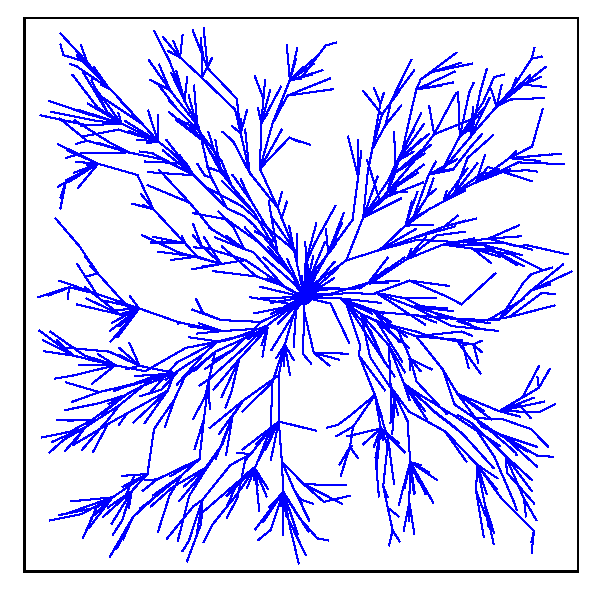
\includegraphics[width=\textwidth]{figChap3/RRTstar_expansion1000.eps}
      \caption{1000 iterations}
      % \label{fig:tiger}
  \end{subfigure}
  ~ %add desired spacing between images, e. g. ~, \quad, \qquad, \hfill etc. 
  %(or a blank line to force the subfigure onto a new line)
  \begin{subfigure}[b]{0.302\textwidth}
      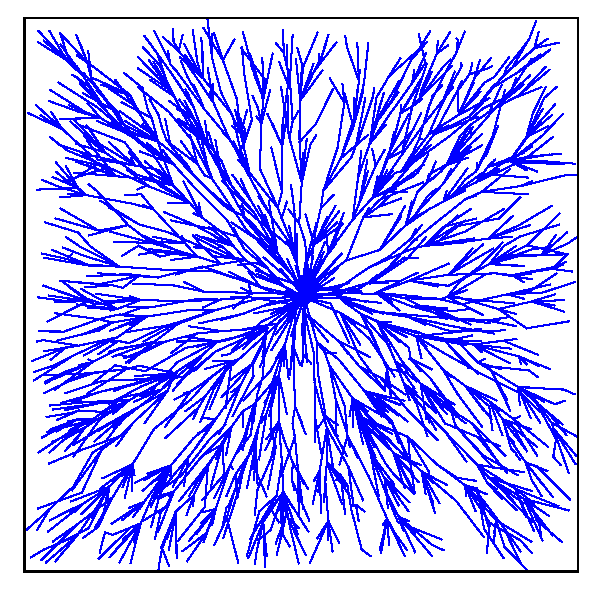
\includegraphics[width=\textwidth]{figChap3/RRTstar_expansion2000.eps}
      \caption{2000 iterations}
      % \label{fig:mouse}
  \end{subfigure}
  \caption{Example of RRT* expansion in 2D $\mathcal{C}$-space.}
  \label{fig:RRTstargrowing}
\end{figure}
%---------------------------------------------------------------------------------
RRT* incorporates a rewiring step that allows the algorithm to dynamically adjust the tree structure, 
thereby promoting the discovery of more optimal paths.
In the Fig. \ref{fig:RRTstargrowing},
the progressive expansion in 2D $\mathcal{C}$-space of the RRT* can be seen.\\[12pt]
%------
Similar to RRT, RRT* begins with an initialization phase and continues with an expansion phase.
However, the key enhancement in RRT* lies in the \textbf{Rewiring phase}, 
aimed at improving the optimality of paths discovered.
This phase can be divided into three parts: Finding Nearest Nodes, 
Choosing Parent Node and Rewiring \ref{fig:RRTstar_explanation}. 
%---------------------------------------------------------------------------------
\begin{figure}[!ht]
  \centering
  \begin{subfigure}[b]{0.45\textwidth}
      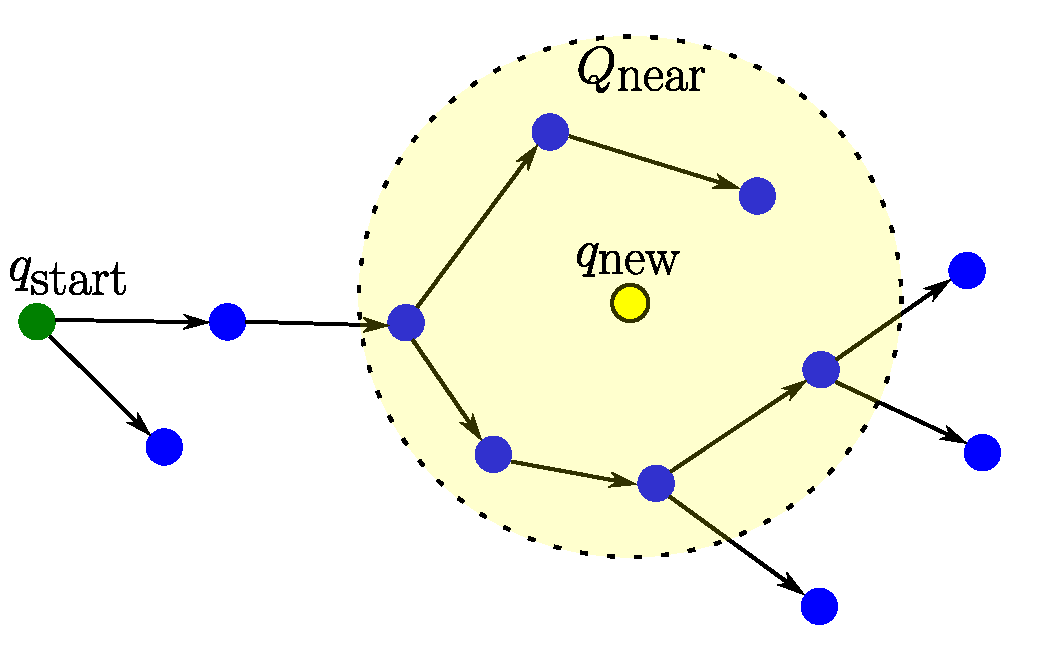
\includegraphics[width=\textwidth]{figChap3/RRTstarNearNodes40pt.pdf}
      \caption{Finding Nearest Nodes.}
      \label{fig:nearest_nodes}
  \end{subfigure}
  ~ %add desired spacing between images, e. g. ~, \quad, \qquad, \hfill etc. 
    %(or a blank line to force the subfigure onto a new line)
  \begin{subfigure}[b]{0.45\textwidth}
      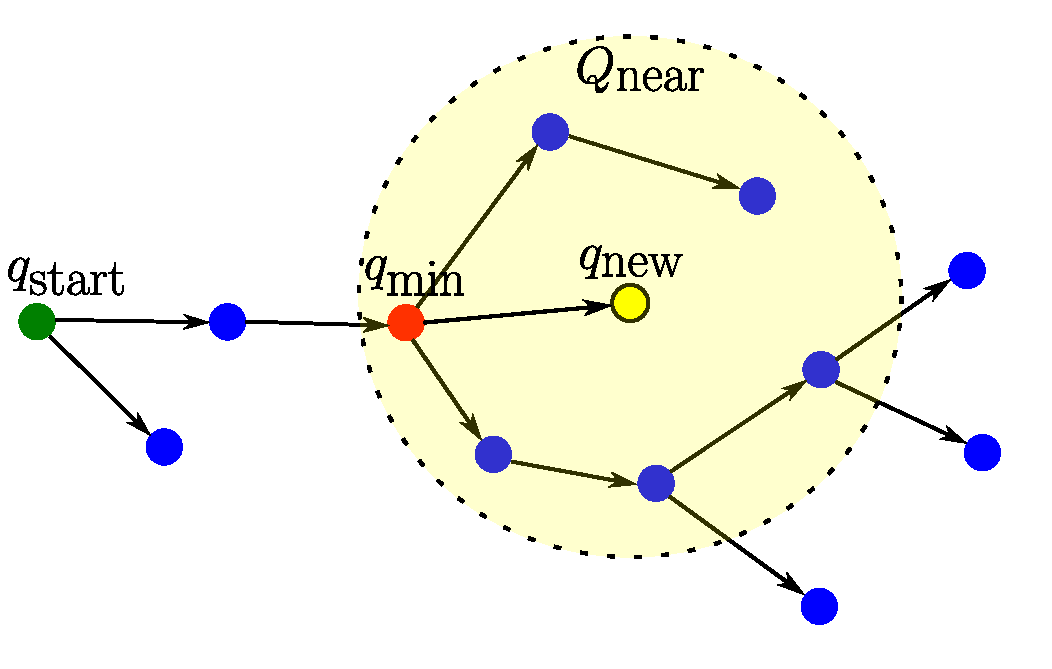
\includegraphics[width=\textwidth]{figChap3/RRTstarChooseParent40pt.pdf}
      \caption{Choosing Parent Node.}
      \label{fig:choose_parent}
  \end{subfigure}
  ~ %add desired spacing between images, e. g. ~, \quad, \qquad, \hfill etc. 
  %(or a blank line to force the subfigure onto a new line)
  \begin{subfigure}[b]{0.45\textwidth}
      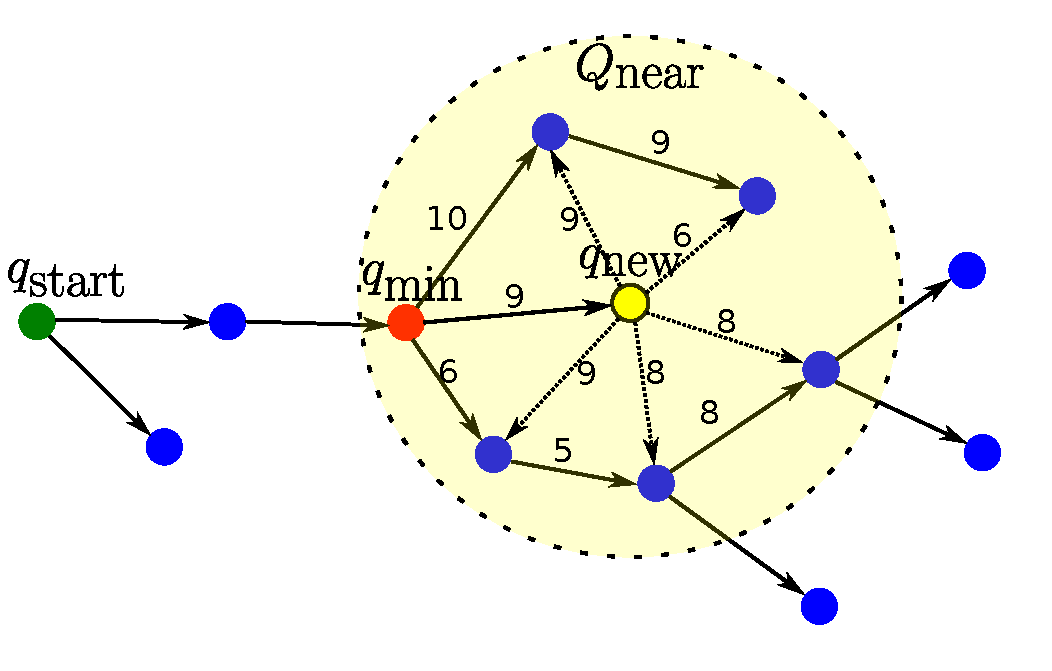
\includegraphics[width=\textwidth]{figChap3/RRTstarCostEvaluation40pt.pdf}
      \caption{Rewiring.}
      \label{fig:rewiring}
  \end{subfigure}
  \begin{subfigure}[b]{0.45\textwidth}
    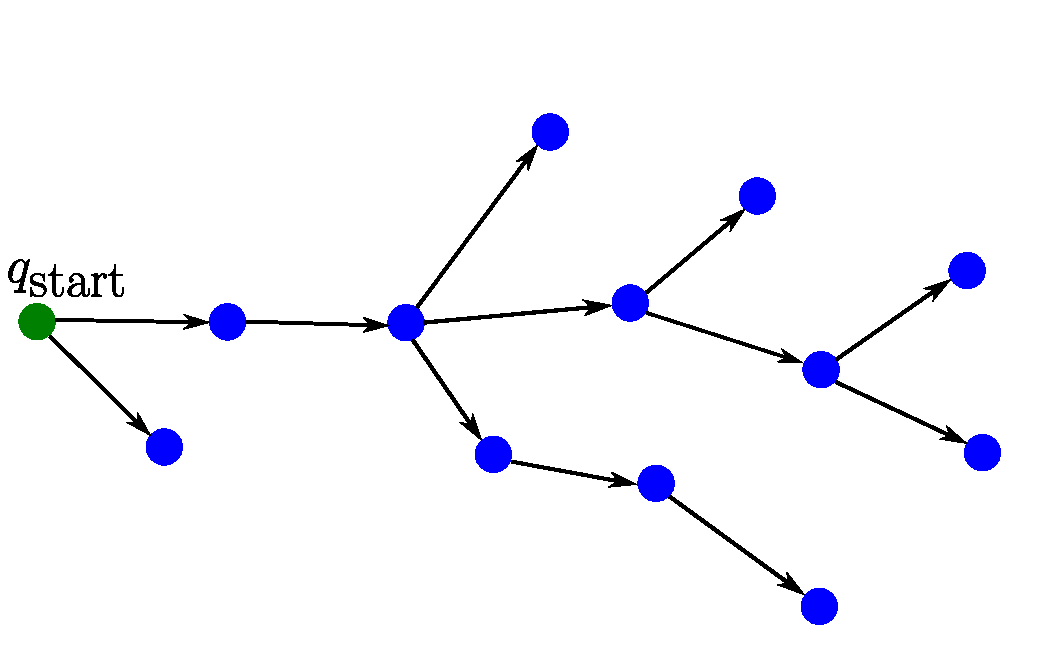
\includegraphics[width=\textwidth]{figChap3/RRTstarFinalLook40pt.pdf}
    \caption{Result.}
    \label{fig:result}
  \end{subfigure}
  \caption{Illustration of the \textbf{Rewiring phase}: 
  The green circle denotes the initial configuration (\( q_{\textit{start}} \)), 
  while the yellow circle represents the new node to be added (\( q_{\textit{new}} \)), 
  along with its transparent yellow circular area with certain radius (\( Q_{\textit{near}} \)). 
  Figure \ref{fig:nearest_nodes} displays the nodes within this circular area. 
  A parent node for the new node, identified by the red circle (\( q_{\textit{min}} \)), 
  can be seen in Figure \ref{fig:choose_parent}. 
  Figure \ref{fig:rewiring} exemplifies the rewiring step, 
  with numerical values indicating the lengths of respective paths from the new node to nearby nodes. 
  Finally, Figure \ref{fig:result} shows the final appearance of the rewired tree.}
  \label{fig:RRTstar_explanation}
\end{figure} 
%---------------------------------------------------------------------------------
\\
Finding Nearest Nodes step involves identifying nearby nodes 
within a certain radius from the new node. 
After identifying nearby nodes, the algorithm proceeds to the Choosing Parent Node step. 
Here, it calculates cost for each node 
relative to the new node and selects the one with the lowest cost. 
This cost evaluation considers both the path from the root to the current node and 
the path from the current node to the nearby node. 
It typically reflects the path length or other user-defined metrics. 
This step is crucial because, 
unlike in RRT where the algorithm simply identifies the nearest node, 
the goal is to find the most optimal node,
which may not always be the nearest one. 
After adding a new node to our hierarchical tree structure, 
the Rewiring step initiates. 
Similar to the Choosing Parent Node step, 
the algorithm evaluates the costs of all possible paths from our new node to all nearest nodes. 
If a new path reduces the cost of the node, the algorithm removes the old path to the node
and adds the new path.
During this process, the rewired node gets a new parent, 
and the old parent, from which the old path originated, may no longer have a child.\\[12pt]
%------
Through these iterative phases, RRT* continuously improves the tree structure, 
resulting in progressively optimal and efficient paths. 
By strategically rewiring the tree, 
RRT* effectively converges towards an optimal solution while 
efficiently exploring the configuration space.\\[12pt]
%------
The RRT* algorithm offers improved optimality over the original RRT, 
making it particularly useful when precision and efficiency are crucial 
considerations in robotic path planning.
As illustrated in Figure \ref{fig:RRTvsRRTstar}, 
RRT* typically generates more direct paths with fewer unnecessary zigzags compared to RRT, 
thereby enhancing path quality.
However, RRT* is more computationally complex, especially compared to RRT, 
which can lead to increased time consumption.\\[12pt]
%---------------------------------------------------------------------------------
%---------------------------------------------------------------------------------
\begin{figure}[!ht]
  \centering
  \begin{subfigure}[b]{0.45\textwidth}
      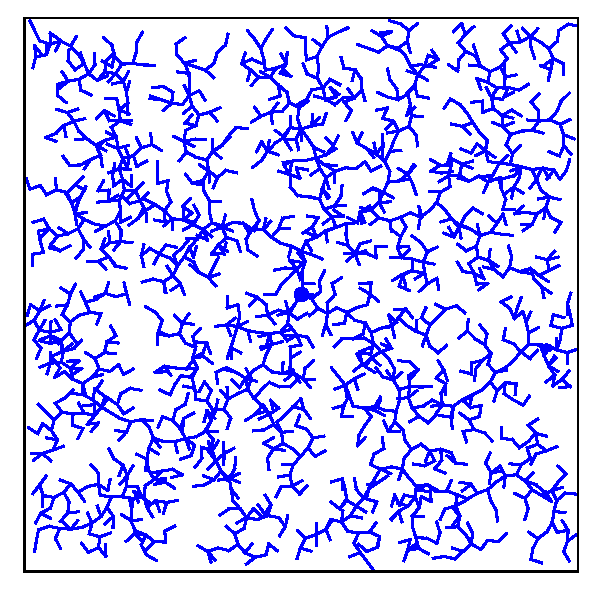
\includegraphics[width=\textwidth]{figChap3/2RRTexpansion2000.eps}
      \caption{RRT.}
      \label{fig:rrt2k}
  \end{subfigure}
  ~ %add desired spacing between images, e. g. ~, \quad, \qquad, \hfill etc. 
    %(or a blank line to force the subfigure onto a new line)
  \begin{subfigure}[b]{0.45\textwidth}
      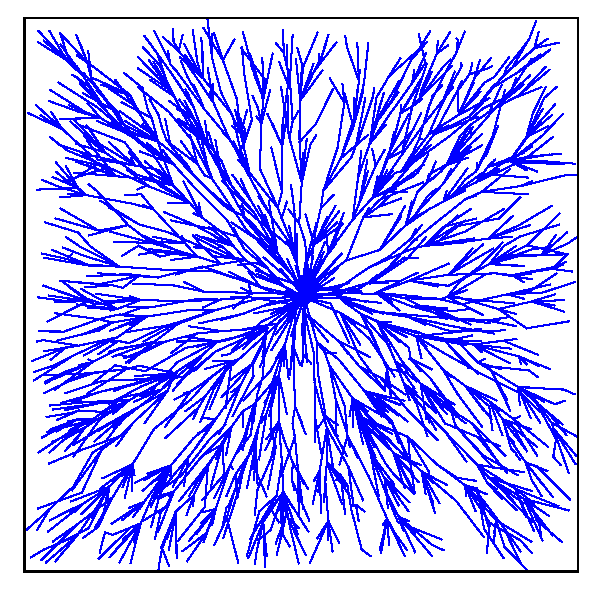
\includegraphics[width=\textwidth]{figChap3/RRTstar_expansion2000.eps}
      \caption{RRT*.}
      \label{fig:rrtstar2k}
  \end{subfigure}  
  \begin{subfigure}[b]{0.45\textwidth}
      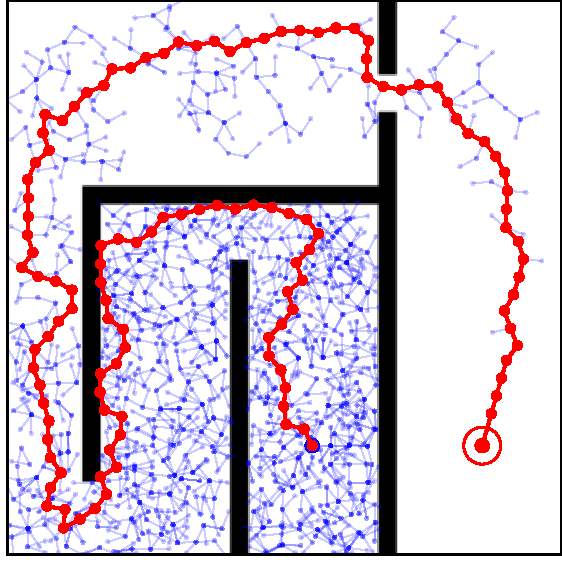
\includegraphics[width=\textwidth]{figChap3/RRT_maze7748i119w.pdf}
      \caption{RRT.}
      \label{fig:rrtMaze}
  \end{subfigure}
  ~ %add desired spacing between images, e. g. ~, \quad, \qquad, \hfill etc.   
    %(or a blank line to force the subfigure onto a new line)
  \begin{subfigure}[b]{0.45\textwidth}
      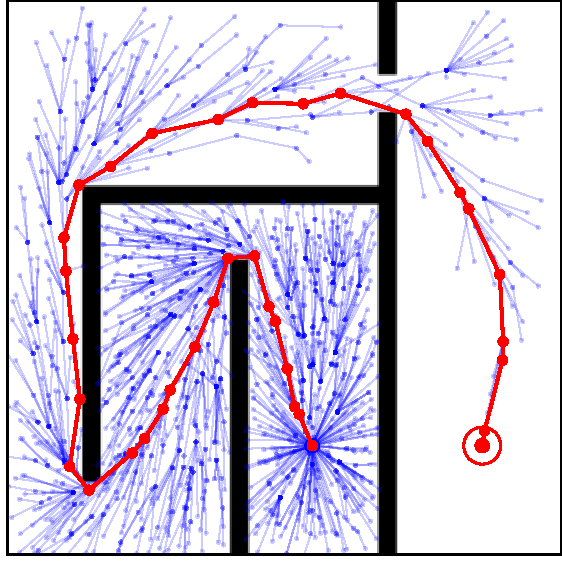
\includegraphics[width=\textwidth]{figChap3/RRTstar_maze_7060i_35w.pdf}
      \caption{RRT*.}
      \label{fig:rrtstarMaze}
  \end{subfigure}  
  \begin{subfigure}[b]{0.45\textwidth}
      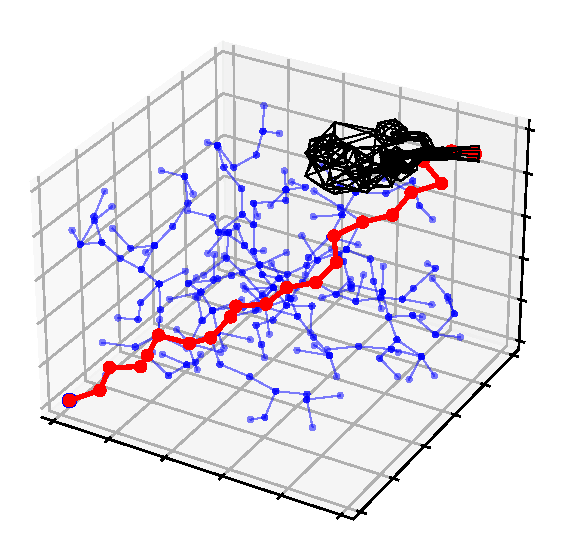
\includegraphics[width=\textwidth]{figChap3/6DRRT_new.pdf}
      \caption{RRT.}
      \label{fig:rrt6D} 
  \end{subfigure}
  ~ %add desired spacing between images, e. g. ~, \quad, \qquad, \hfill etc. 
    %(or a blank line to force the subfigure onto a new line)
  \begin{subfigure}[b]{0.45\textwidth}
      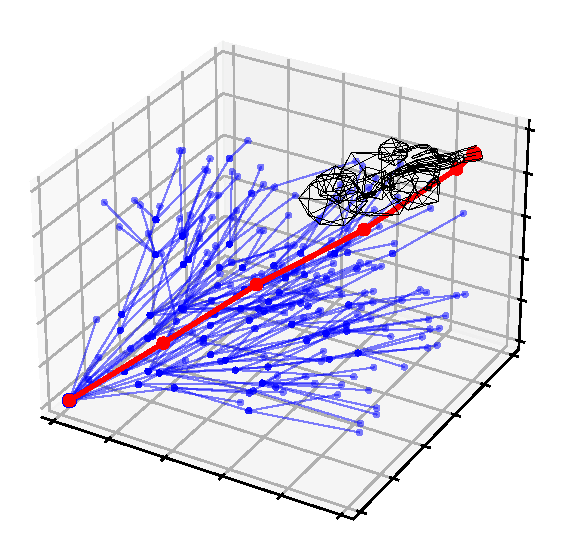
\includegraphics[width=\textwidth]{figChap3/6DRRTstar3_new.pdf}
      \caption{RRT*.}
      \label{fig:rrtstar6D}
  \end{subfigure} 
  \caption{Comparison in 2D $\mathcal{C}$-space without obstacles in \ref{fig:rrt2k} 
  and \ref{fig:rrtstar2k} with obstacles in \ref{fig:rrtMaze} and \ref{fig:rrtstarMaze}.
  Comparison in 6D $\mathcal{C}$-space with an object represented as a tree in \ref{fig:rrt6D} and \ref{fig:rrtstar6D}.}
  \label{fig:RRTvsRRTstar}
\end{figure}
%---------------------------------------------------------------------------------
\begin{algorithm}[H]
  \caption{Rapidly-exploring Random Tree Star (RRT*)}
  \label{alg:rrt_star}
  \SetAlgoNlRelativeSize{0}
  
  \KwData{Start configuration $q_{\text{start}}$, Number of iterations $K$, Radius $r$}
  \KwResult{RRT* tree $T$}
  \vspace{0.1cm}
  \hrule
  \vspace{0.2cm}
  $T \leftarrow$ InitializeTree($q_{\text{start}}$)\;
  
  \For{$k \leftarrow 1$ \KwTo $K$}{
    $q_{\text{rand}} \leftarrow$ RandomConfiguration()\;
    $q_{\text{near}} \leftarrow$ NearestNode($T, q_{\text{rand}}$)\;
    $q_{\text{new}} \leftarrow$ Steer($q_{\text{near}}, q_{\text{rand}}$)\;
    
    \If{ObstacleFree($q_{\text{near}}, q_{\text{new}}$)}{
      $Q_{\text{near}} \leftarrow$ NearNodes($T, q_{\text{new}}, r$)\;
      $q_{\text{min}} \leftarrow$ ChooseParent($Q_{\text{near}}, q_{\text{new}}$)\;
      $T \leftarrow$ AddNode($q_{\text{new}}, q_{\text{min}}$)\;
      $T \leftarrow$ Rewire($T, Q_{\text{near}}, q_{\text{new}}$)\;
    }
  }

  \Return $T$\; 
\end{algorithm} 

%---------------------------------------------------------------------------------
%---------------------------------------------------------------------------------
%---------------------------------------------------------------------------------
\clearpage 
\section{Probabilistic RoadMaps (PRM)}
The Probabilistic Roadmap (PRM)~\cite{Kavraki1996PRM} algorithm is a 
popular motion planning technique used in robotics to find feasible paths 
for robots operating in complex, high-dimensional spaces. 
Unlike traditional grid-based approaches, 
PRM operates by constructing a roadmap of the configuration space, 
which is then used to efficiently search for valid paths.
The roadmap generated by PRM can be likened to a street network in a city. 
Just as roads connect various locations in a city, 
edges in the PRM roadmap connect different configurations in the configuration space. 
This analogy helps to conceptualize how the PRM algorithm constructs a network of 
feasible paths for the robot to navigate through the environment.
\\[12pt]
The PRM algorithm consists of the following main steps: 
Roadmap Construction, Neighborhood Search, Edge Connection, and Path Planning.
A pseudocode of construction step is shown in Algorithm \ref{alg:prm_constraction}.
%---------------------------------------------------------------------------------
\begin{figure}[!ht]
  \centering
  \begin{subfigure}[b]{0.45\textwidth}
      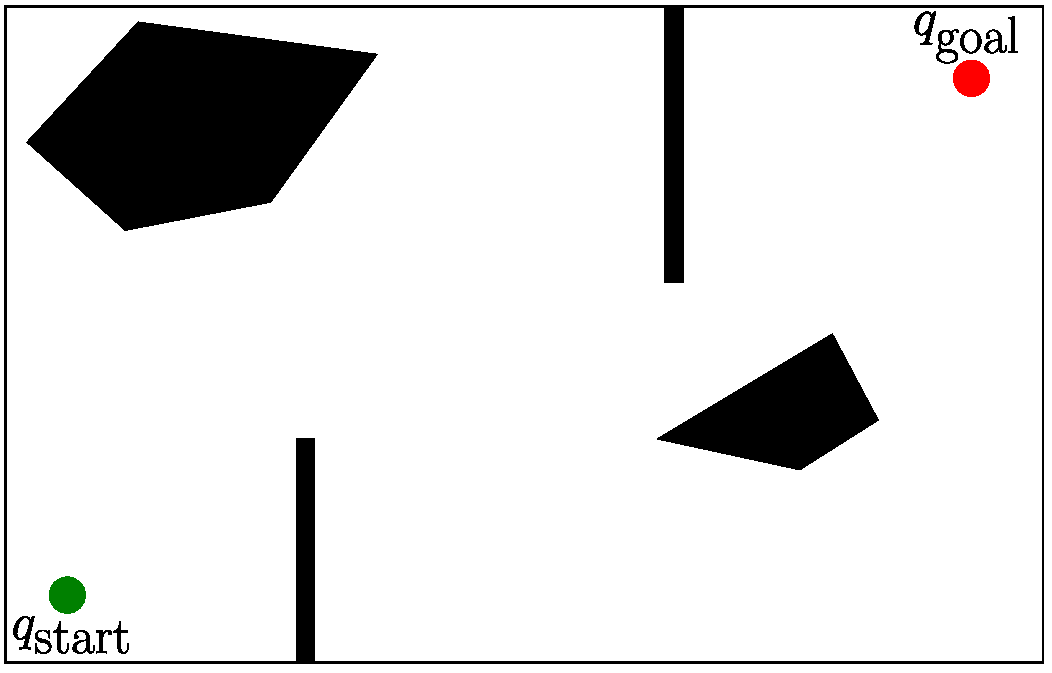
\includegraphics[width=\textwidth]{figChap3/PRMmaze40pt.pdf}
      \caption{2D $\mathcal{C}$-space.}
      \label{fig:prm_maze}
  \end{subfigure}
  ~ %add desired spacing between images, e. g. ~, \quad, \qquad, \hfill etc. 
    %(or a blank line to force the subfigure onto a new line)
  \begin{subfigure}[b]{0.45\textwidth}
      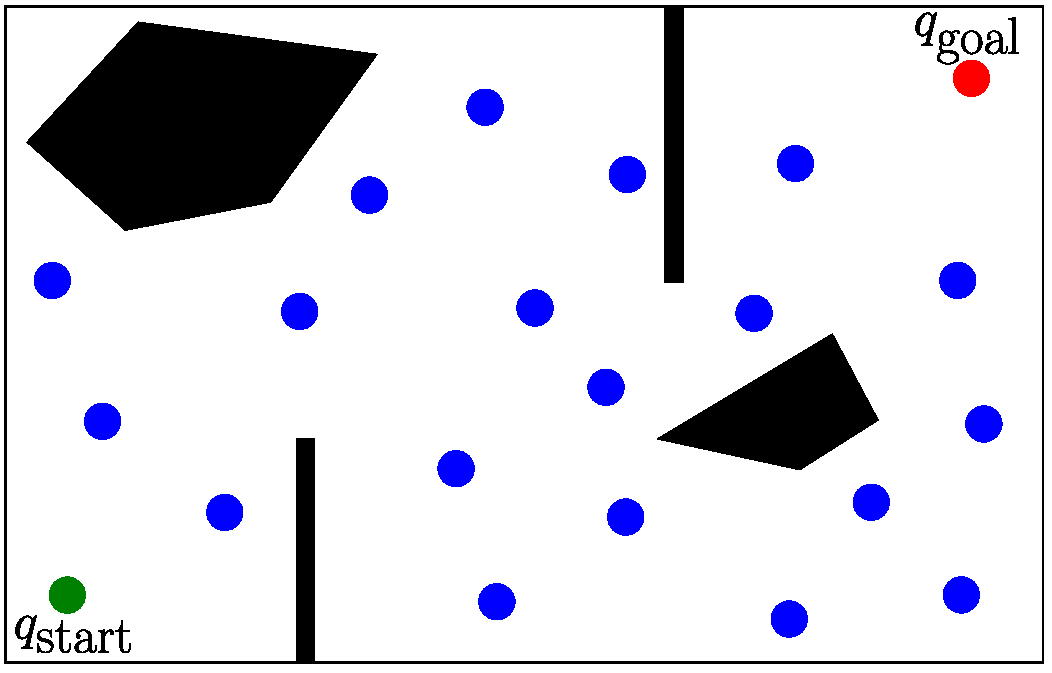
\includegraphics[width=\textwidth]{figChap3/PRMsamplePoints40pt.pdf} 
      \caption{Roadmap Construction.}
      \label{fig:random_points}
  \end{subfigure}
  ~ %add desired spacing between images, e. g. ~, \quad, \qquad, \hfill etc. 
  %(or a blank line to force the subfigure onto a new line)
  \begin{subfigure}[b]{0.45\textwidth}
      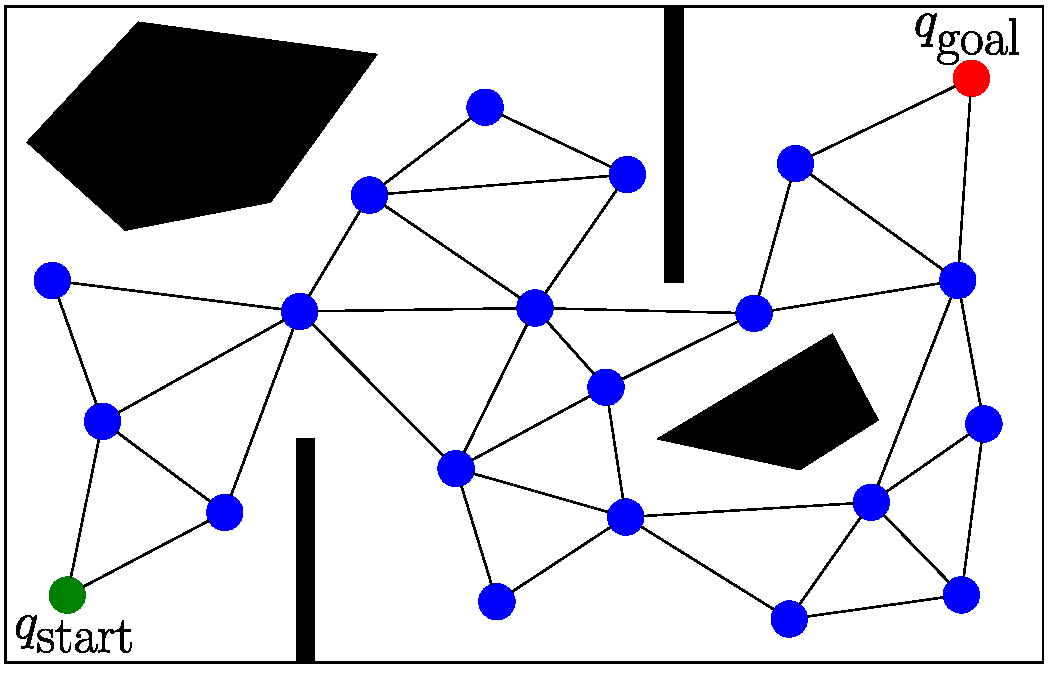
\includegraphics[width=\textwidth]{figChap3/PRMconnecting40pt.pdf}
      \caption{Edge Conecting.}
      \label{fig:edges}
  \end{subfigure}
  \begin{subfigure}[b]{0.45\textwidth}
    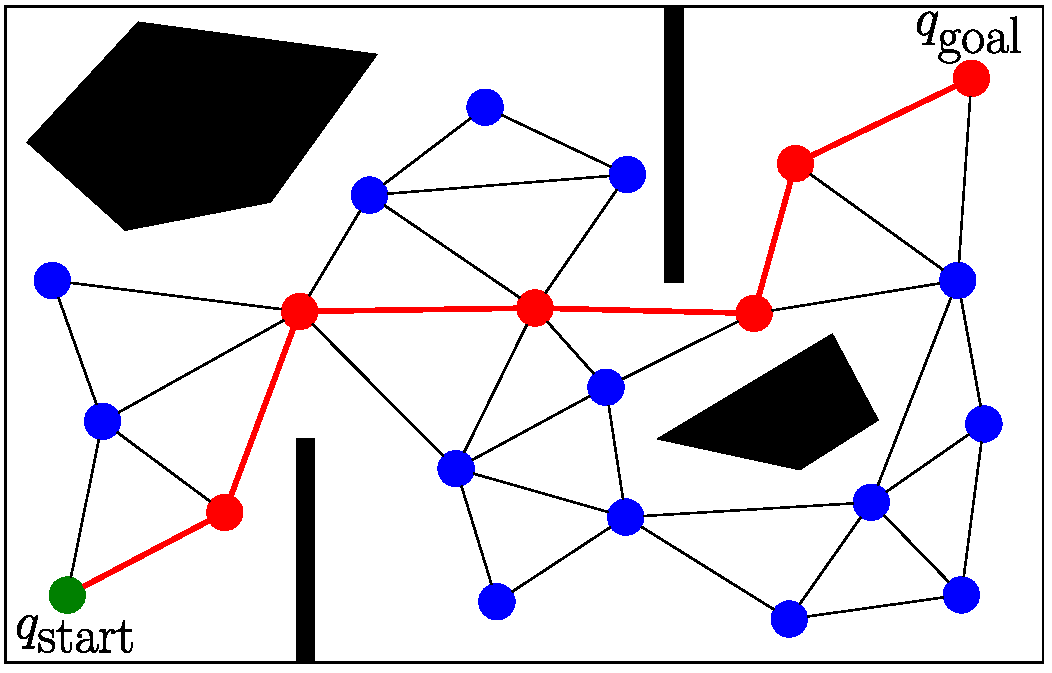
\includegraphics[width=\textwidth]{figChap3/PRMpathFinding40pt.pdf}
    \caption{Path Planning.}
    \label{fig:prm_path_planning}
  \end{subfigure}
  \caption{
    In the 2D $\mathcal{C}$-space depicted in Figure \ref{fig:prm_maze}, 
    obstacles are represented in black. 
    The initial configuration ($q_{\text{start}}$) is indicated by a green circle, 
    while the goal configuration ($q_{\text{goal}}$) is marked with a red circle.
    Additionally, randomly sampled valid configurations appear as blue circles \ref{fig:random_points}. 
    The connections between these configurations can be seen in Figure \ref{fig:edges}.
    The path discovered between the start and goal configurations is highlighted in red \ref{fig:prm_path_planning}.}
  \label{fig:PRM_explanation}
\end{figure} 
%---------------------------------------------------------------------------------
\\
Roadmap Construction involves randomly sampling configurations from the configuration space and 
checking each sampled configuration for collision with obstacles. 
Valid configurations are added to the roadmap.
In the Neighborhood Search step, for each sampled configuration, 
a set of neighboring configurations is identified. 
These neighbors serve as potential candidates for connecting edges in the roadmap.
In the Edge Connection step, 
pairs of neighboring configurations are evaluated to determine 
if an edge should be added between them in the roadmap. 
This evaluation typically involves checking for collision-free paths between the configurations.
Finally, in the Path Planning step, once the roadmap is constructed, 
path planning becomes a graph search problem. 
Algorithm such as A*~\cite{Hart1968Astar} is commonly used to find the shortest path 
between the start and goal configurations in the roadmap.
These steps can be seen in Figure \ref{fig:PRM_explanation}.
\\[12pt]
PRM can handle complex, high-dimensional configuration spaces and 
environments with obstacles of varying shapes and sizes.
Its straightforward implementation ensures efficient and fast solution finding.
However, the quality of the roadmap depends heavily on the sampling strategy and 
collision checking accuracy. 
Poorly constructed roadmaps may lead to suboptimal or infeasible paths.
Moreover, PRM encounters challenges when navigating through narrow passages, 
as the likelihood of sampling configurations capable of traversing tight gaps diminishes 
with the decreasing gap.\\[12pt]
%------
Despite its drawbacks, 
PRM remains a widely used and effective approach for motion planning in robotics, F
particularly in scenarios with complex environments and obstacles.\\
%---------------------------------------------------------------------------------

\begin{algorithm}[H]
  \caption{Probabilistic Roadmap (PRM) construction step}
  \label{alg:prm_constraction} 
  \KwData{Start configuration $q_{\text{start}}$, Number of iterations $K$}
  \KwResult{PRM graph $G$}
  \vspace{0.1cm}
  \hrule
  \vspace{0.2cm}
  Initialize graph $G$ with vertices $V$ and edges $E$\;
  \For{$i \gets 1$ \KwTo $K$}{
    $q_{\text{rand}} \leftarrow$ a randomly choosen free configuration\;
    $Q_{\text{near}} \leftarrow$ a set of candidate neighbors of $q_{\text{rand}}$ chosen from $V$\;
    $V \gets V \cup \{q_{\text{rand}}\}$\;
    \For{$q \in Q_{\text{near}}$}{
      \If{not $\text{SameConnectedComponent}(q_{\text{rand}}, q)$}{
        $E \gets E \cup \{(q_{\text{rand}}, q)\}$\;
        \textbf{update} connected components in $G$\;
      }
    }
  }
  \Return $G$\;
\end{algorithm}
%---------------------------------------------------------------------------------
%---------------------------------------------------------------------------------
\section{Informed RRT*}
Informed RRT*~\cite{Gammell2018InformedRRTstar} extends the capabilities of the RRT* algorithm 
by addressing the challenges inherent in exploring high-dimensional configuration spaces 
with greater efficiency. 
It achieves this by integrating heuristic guidance, 
typically through cost-to-go estimates or other informed sampling strategies, 
to direct exploration towards regions more likely to yield the optimal solution.
The cost-to-go refers to the estimated cost or distance from a given 
configuration to reach a goal configuration in a path planning problem.  
Building upon the fundamental principles of RRT*, 
Informed RRT* retains its core mechanics of incremental tree growth and probabilistic sampling. 
However, unlike traditional RRT*, 
which uniformly samples configurations at random, 
Informed RRT* employs informed sampling techniques to prioritize sample 
points in areas with lower estimated costs or higher likelihood of containing 
the optimal solution.  
\\[12pt]
In Informed RRT*, 
hyperspheroid are often utilized as a representation of the cost-to-go heuristic. 
These hyperspheroids encapsulate regions of the configuration space that are likely 
to contain the optimal solution. 
By leveraging these hyperspheroids,   
This utilization of hyperspheroids enables Informed RRT* to efficiently 
explore high-dimensional spaces and converge towards the optimal solution more effectively 
than traditional RRT* algorithms.
%---------------------------------------------------------------------------------
\begin{figure}[!ht]
  \centering 
      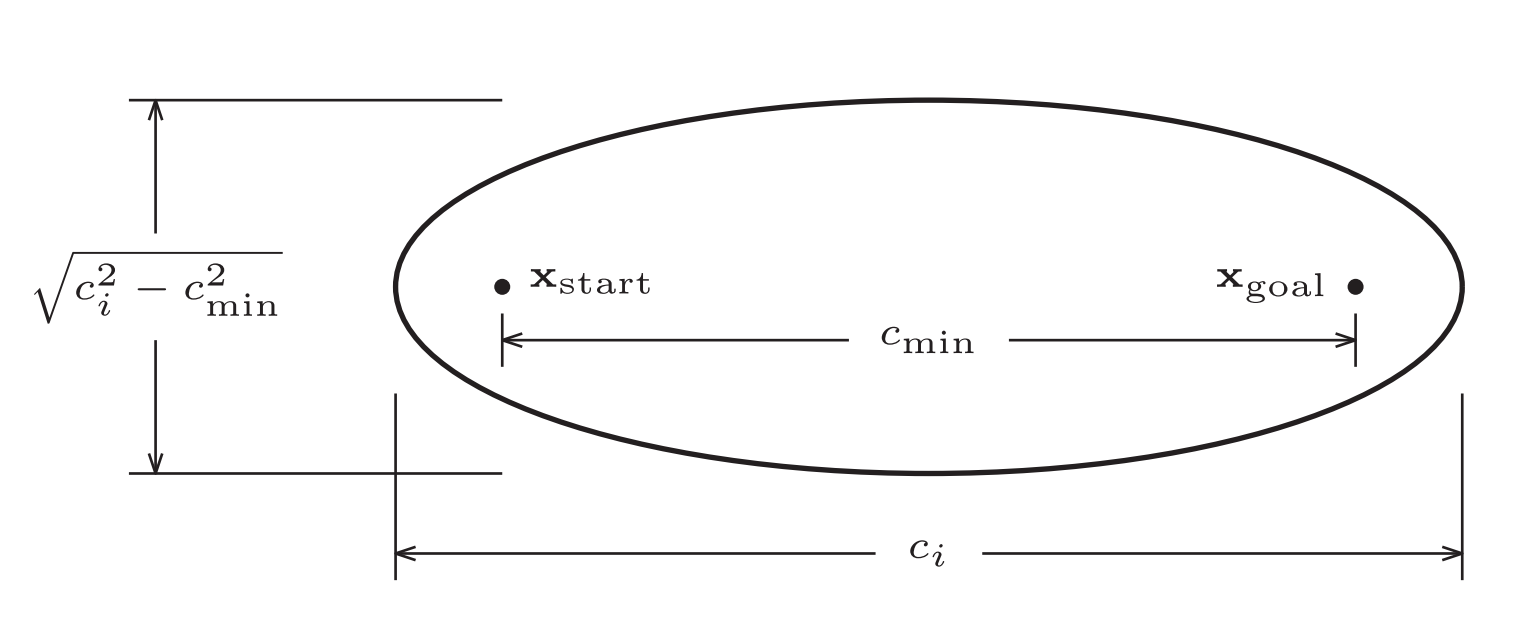
\includegraphics[width=\textwidth]{figChap3/InformedRRTstar_elips.png}
      \caption{An example of a two-dimensional prolate hyperspheroid.}
      \label{fig:elips}  
\end{figure} 
%---------------------------------------------------------------------------------
\\[12pt]
The prolate hyperspheroid (\ref{fig:elips}) is defined by its focal points 
at start configuration \( \textbf{x}_{\text{start}} \) and goal configuration 
\( \textbf{x}_{\text{goal}} \), a transverse diameter of current solution cost \( c_i \), 
and conjugate diameters of \(\sqrt{( c_i^2 - c_{\text{min}}^2)} \), 
where \[ c_{\text{min}} := \| \textbf{x}_{\text{goal}} - \textbf{x}_{\text{start}} \|_2 \]
is the theoretical minimum cost.
%---------------------------------------------------------------------------------
%---------------------------------------------------------------------------------
\section{\texorpdfstring{RRT sharp (RRT$^\#$)}{Title without Superscript}}
RRT sharp (RRT$^\#$)~\cite{arslan2012rrtsharp} is a sampling-based motion planning algorithm, 
which is based on Rapidly Exploring Random Graphs (RRG)~\cite{Karaman2009RRG}. 
The RRT$^\#$ algorithm utilizes informed sampling techniques to bias the selection of sample 
points towards relevant regions with lower estimated costs or higher likelihoods of containing the optimal solution. 
This information enhances the convergence speed of the algorithm and 
enables more efficient exploration of the obstacle-free space.
\\[12pt]
To find the relevant region, the following formula is used:
\[
X_{\text{rel}} = \{ x \in X_{\text{free}} : g^*(x) + h(x) < g^*(x^*_{\text{goal}}) \}
\]
where \( x^*_{\text{goal}} \) is the point in the goal 
region with the lowest optimal cost-to-come value, 
\( g^*(x) \) is the optimal cost-to-come value of 
point \( x \), and \( h(x) \) is the estimate of the 
optimal cost moving from \( x \) to the goal region \( X_{\text{goal}} \).
If a point \( x \) is within the region \( X_{\text{goal}} \), \( h(x) \) is equal to zero.
%---------------------------------------------------------------------------------
%---------------------------------------------------------------------------------
\section{\texorpdfstring{RRT$^X$ static}{Title without Superscript}}
RRT$^X$~\cite{Otte2015RRTX} is an algorithm primarily engineered to navigate dynamic environments, 
where configurations of obstacles are unpredictable, demanding real-time adaptability.
In this study, 
the focus is on delving into the static adaptation of RRT$^X$, named RRT$^X$ static. 
Tailored for scenarios where environmental dynamics are stable.
\\[12pt]
The implementation of the RRT$^X$ static algorithm closely resembles that of RRT$^\#$, 
with the addition of a single parameter, 
$\epsilon$, representing the minimum threshold for cost improvement required to rewire the tree. 
In simpler terms, 
$\epsilon$ specifies the minimum amount by which a new path must improve over the existing path 
for the algorithm to justify rewiring the tree.
%---------------------------------------------------------------------------------
%---------------------------------------------------------------------------------
\section{Motion Planning Networks (MPNet)}
Motion Planning Networks (MPNet)~\cite{Ahmed2019MotionPlanningNetworks} is an 
innovative learning-based neural planner.  
MPNet  leverage neural networks to learn optimal path planning strategies, 
making them highly efficient in navigating complex environments.  
One of the primary reasons for using MPNets is their ability to 
significantly reduce computation time compared to traditional methods like RRT*. 
This speed advantage makes MPNets particularly suitable for real-time applications where 
rapid decision-making is essential.
\\[12pt]
According to the documentation \cite{Ahmed2019MotionPlanningNetworks}, 
MPNet comprises two key components: the Planner Network (Pnet) and the Encoder Network (Enet). 
Enet processes information about the surrounding environment of the robot, 
including a raw point cloud. 
A raw point cloud refers to a collection of data points in a 3D space that 
represents the surface of an object or scene.
The output of Enet is a latent space embedding of this raw point cloud information. 
Pnet utilizes the encoding of the environment, 
along with information about the current state and goal state of the robot, 
to generate samples for path or tree generation.
\\[12pt]
Let the environment surrounding the robot, 
referred to as the workspace, 
be denoted as \(\mathcal{X} \subseteq \mathbb{R}^m\), where \(m\) is the workspace dimension. 
This workspace encompasses both obstacle regions \(\mathcal{X}_{obs}\) and 
obstacle-free regions \(\mathcal{X}_{free} = \mathcal{X} \setminus \mathcal{X}_{obs}\). 
MPNet plans feasible, 
near-optimal paths using raw point-cloud of obstacles \(x_{obs} \subset \mathcal{X}_{obs}\). 
Similar to other planning algorithms, 
there is an assumed availability of a collision-checker 
that verifies the feasibility of MPNet-generated paths based on \(\mathcal{X}_{obs}\).
Precisely, Enet, parameterized by \( \theta^e \), 
processes the raw point cloud information \( x_{obs} \) and 
compresses it into a latent space \(Z\). 
\[
  Z \leftarrow \text{Enet}(x_{obs}; \theta^e)
\]
Pnet, parameterized by \( \theta^p \), utilizes this latent space encoding \(Z\), 
as well as the current or initial configuration \(c_t \in \mathcal{C}_{\text{free}}\) and 
the goal configuration \(c_{goal} \subset \mathcal{C}_{\text{free}}\) of the robot, 
to produce a trajectory through incremental generation of 
states \( \hat{c}_{t+1} \).
\[
  \hat{c}_{t+1} \leftarrow \text{Pnet}(Z, c_t, c_{goal}; \theta^p)  
\]
Together, these neural networks enable MPNet to plan paths efficiently in complex environments.
\\[12pt]
One notable feature of MPNet is its integration of classical 
sample-based planners in a hybrid approach, 
which allows for worst-case theoretical guarantees while retaining computational efficiency and 
optimality improvements. 
Additionally, an active continual learning approach is presented to train MPNet models, 
enabling learning from streaming data and expert demonstrations as needed, 
thus reducing training data significantly.
\\[12pt]
Despite their numerous advantages, MPNets also have some limitations. 
The quality of the path generated by MPNets heavily depends on the training data and 
the accuracy of the learned heuristic. 
Poorly trained MPNets may produce suboptimal or infeasible paths. 
\\[12pt]
In the context of this thesis, 
MPNets provide valuable insights into the diversity of path planning methodologies. 
Moreover, through the integration of neural networks, 
which is a fundamental machine learning technique, 
MPNets aim to enhance sampling-based methods. 
Consequently, they are particularly relevant for understanding the existing methods and 
their advancements in the area of sampling-based approaches.

%---------------------------------------------------------------------------------
%---------------------------------------------------------------------------------
\section{Summarize}
In the Related Works chapter, various approaches relevant to this thesis were explored, 
including Motion Planning Networks (MPNet). 
MPNet serves as a notable example, indicating the potential for improvement in 
sampling-based planners. 
Sampling-based methods such as RRT, RRT*, and PRM are widely used in path planning. 
However, they all exhibit limitations when navigating through narrow passages and 
environments dense with obstacles. 
These limitations stem from their random sampling strategy, 
which often results in scenarios with narrow passages and dense obstacle spaces, 
leading to the generation of configurations within obstacle space. 
Consequently, this leads to unnecessary collision checking for inappropriate configurations. 
As a result, there is an increase in computational time and a decrease in the probability 
of sampling configurations capable of traversing tight gaps as the gap size decreases. 
To address these challenges and achieve improvements in the performance of sampling-based methods,
akin to those seen in MPNet, 
the proposed solution to the problem will be provided in the subsequent Chapter \ref{chap:Improving RRT*}.
This method will be compared to its performance with RRT*, RRT$^X$ static, RRT$^\#$ and Informed RRT*.
% \section{Comparison of RRT and RRT* algorithms}
% In this section, the focus will be on comparing RRT with its enhanced variant, RRT*.
% \\\\ 
% During the search for the first feasible path in the configuration space, 
% RRT is typically faster than RRT*. 
% It is evident from the provided Fig. 
% \hyperref[fig:RRTvsRRT*Maze1]{\ref*{fig:RRTvsRRT*Maze1}} and 
% Fig. \hyperref[fig:RRTvsRRT*Maze2]{\ref*{fig:RRTvsRRT*Maze2}} that RRT required less number of iterations to find a path compared to RRT*.
% However, the path found by RRT* is often shorter.
% \\\\
% Another aspect of comparison involves observing how the algorithms explore 
% the configuration space over a significant number of steps. 
% The provided Fig. \hyperref[fig:RRTvsRRT*10k]{\ref*{fig:RRTvsRRT*10k}} illustrates that RRT* 
% tends to have more direct paths without unnecessary zigzags compared to RRT.
%---------------------------------------------------------------------------------
% \begin{figure}
% \centerline{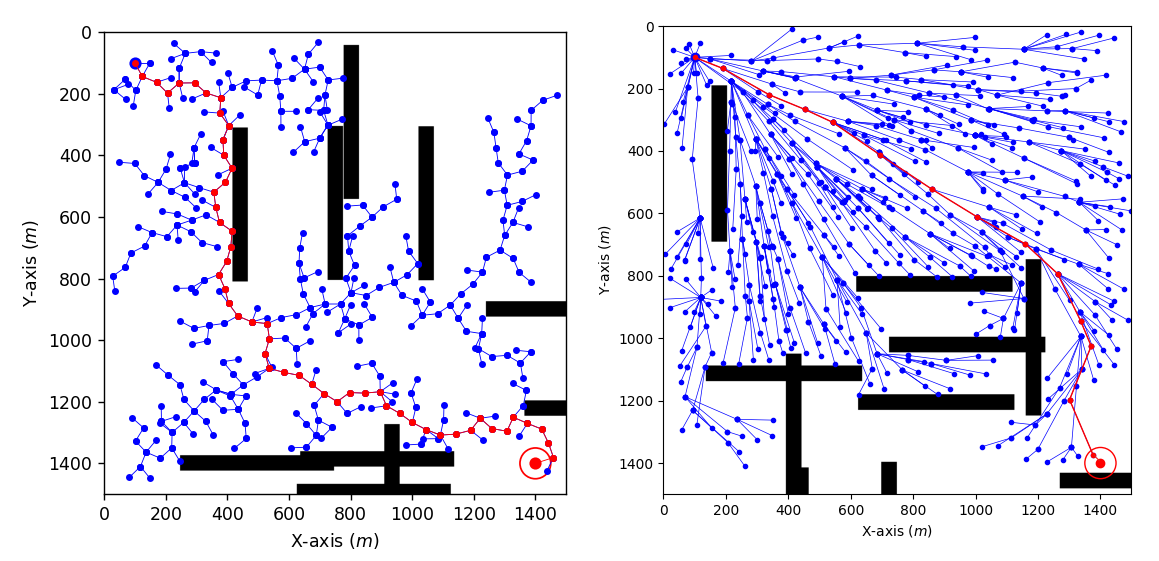
\includegraphics[width=\columnwidth]{figures/RRTvsRRTstar_maze2.png}}
% \caption{RRT and RRT* Maze1} 
% \label{fig:RRTvsRRT*Maze1}
% \end{figure}



%---------------------------------------------------------------------------------
%----------------------------MAYBE ADD TO APPENDIX--------------------------------
% \section{Implementation in 2D space}

% In this section, the practical implementation of the RRT and RRT* algorithms 
% in a 2D configuration space is outlined. 
% The objective is to represent the robot and obstacles as a list of coordinates 
% representing the vertices of the polygon, 
% allowing objects to have arbitrary shapes by specifying the coordinates of their vertices.  
% \\\\ 
% Collision detection between the robot and obstacles is accomplished 
% by utilizing the \texttt{intersects} method of the \texttt{Polygon} class 
% from the \texttt{shapely.geometry} library.  
% To ensure accurate collision checking during motion, 
% linear interpolation of the path is conducted, 
% with collision detection performed at each interpolated point.
% \\\\
% In Fig. \hyperref[fig:RRTstar2D_mazes]{\ref*{fig:RRTstar2D_mazes}} can be seen 
% how the algorithm attempted to navigate around obstacles. 
% Additionally, the flexibility to create any necessary shapes is evident.
% \\\\
% Visualization is achieved using the \texttt{matplotlib} library.
%---------------------------------------------------------------------------------
% \begin{figure} 
%     \centering
%     \begin{minipage}[t]{0.45\textwidth}
%         \centering
%         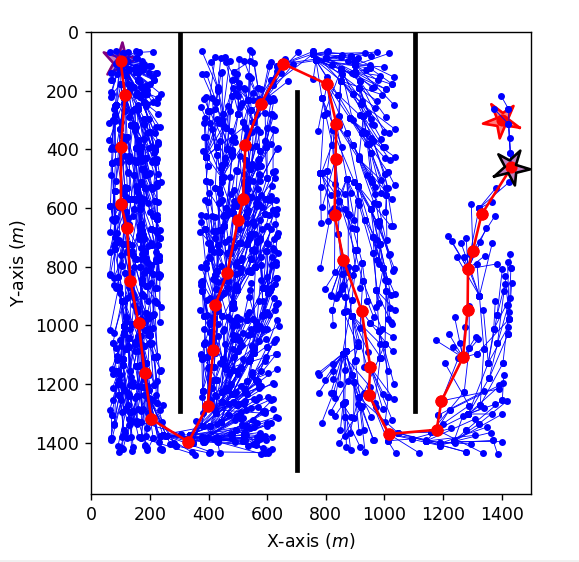
\includegraphics[width=1.2\textwidth]{figures/RRTstar2D.png}  
%     \end{minipage}
%     \hfill
%     \begin{minipage}[t]{0.45\textwidth}
%         \centering
%         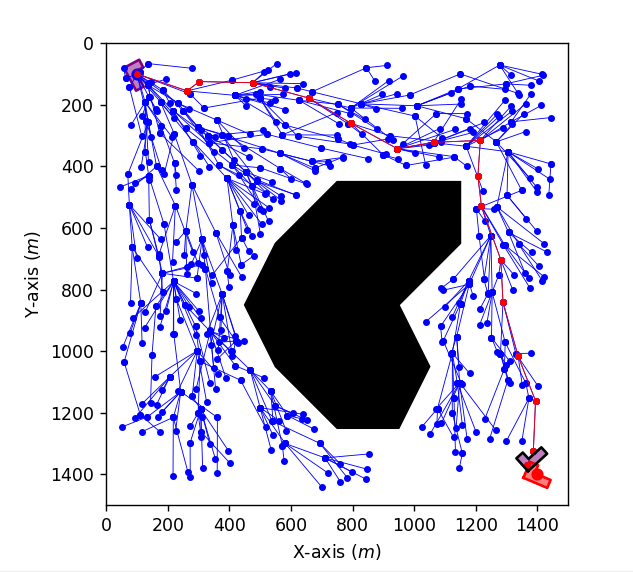
\includegraphics[width=1.31\textwidth]{figures/RRTstar2D_2.png} 
%     \end{minipage} 
%     \caption{RRT* 2D Maze1 and Maze2} 
%     \label{fig:RRTstar2D_mazes}
% \end{figure}
 

%---------------------------------------------------------------------------------
%---------------------------------------------------------------------------------
%---------------------------------------------------------------------------------
% \section{Implementation in 3D space}

% In the 3D implementation of the algorithm, 
% the fundamental structure remains largely the same as in 2D.
% However, there are some key additions, 
% primarily the inclusion of new parameters such as the Z-component and rotations along the X, Y, and Z axes.
% \\\\ 
% To represent objects in the 3D space, a shift from polygons to object files (\texttt{.obj}) has been introduced. 
% These files, which can be easily sourced from the internet, provide a structured representation of 3D objects. 
% All objects must be represented as triangles. 
% That is, each face of an object should be represented using three vertices in the form of triangles.  
% For example, a cube in Fig. \hyperref[fig:cube]{\ref*{fig:cube}}.
% The capability to load more difficult objects, like a tree, is a notable advantage of using \texttt{.obj} files, 
% as demonstrated in Fig. \hyperref[fig:tree]{\ref*{fig:tree}}.
% \\\\
% For 3D collision detection, 
% the preference is to use the \texttt{RAPID} library instead of the \texttt{shapely.geometry} library, 
% given its significantly faster detection capabilities. 
% \texttt{RAPID}(Robust and Accurate Polygon Interference Detection) \cite{gottschalk1997rapid}, written in \texttt{C++}, 
% is a powerful tool for collision detection in 3D environments. 
% It provides a narrow and easy-to-use API(Application Programming Interface) for programmers, 
% facilitating the detection of intersections between polygons in various applications 
% such as physically based modeling, virtual prototyping, and CAD.  
% \\\\ 
% Visualization is also achieved using the \texttt{matplotlib} library.


%---------------------------------------------------------------------------------

% \begin{figure}
% \centerline{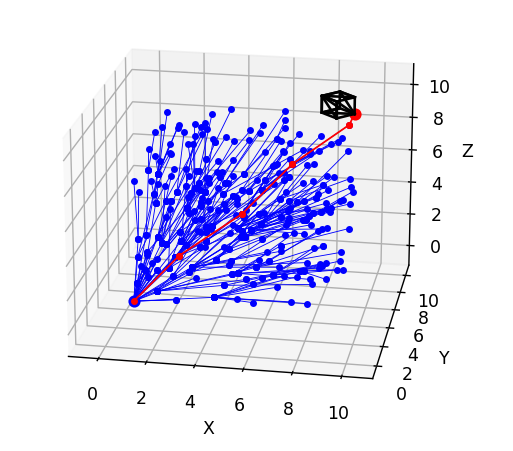
\includegraphics[width=0.7\columnwidth]{figures/RRTstar3Dcube.png}}
% \caption{Cube representation} 
% \label{fig:cube}
% \end{figure}  
%---------------------------------------------------------------------------------
%---------------------------------------------------------------------------------
%---------------------------------------------------------------------------------
\chapter{Improving RRT* algorithm using machine learning method}  
\label{chap:Improving RRT*} 
% \textbf{Here I will explain what i use from this~\cite{arslan2015machine}. The most part will be the same
% as from main documentation which from i use ML methods. add here fotos of the algorithm work. 
% and add fotos of 3D config space.}
%---------------------------------------------------------------------------------
%---------------------------------------------------------------------------------
In this chapter, 
the proposed solution to the challenge formulated in 
Chapter \ref{chap:Task formulation} will be explained. 
As previously mentioned, 
the focus on generating samples within 
the \( \mathcal{C}_{\text{free}} \) ensures that configurations 
within the \( \mathcal{C}_{\text{obs}} \) space are not sampled. 
This strategic approach minimizes the number of iterations required, 
as samples within the \( \mathcal{C}_{\text{obs}} \) space invariably result in collisions, 
thus slowing down the process of achieving the optimal solution. 
To solve this challenge, 
the chapter will delve into the process of learning the configuration space, 
elucidating the proposed sample strategy and its integration into the RRT* algorithm. 
Furthermore, the extension of this approach to the 3D $\mathcal{C}$-space will be discussed.
\\[12pt]
The main idea and implementation of the approach presented in 
this chapter are inspired by the work of~\cite{arslan2015machine}. 
Consequently, many of the terminologies and concepts will closely resemble 
those expounded upon in the referenced work.
%---------------------------------------------------------------------------------
%---------------------------------------------------------------------------------
\section{Approach} 
To provide further clarity, 
it is imperative to introduce some new terminology. 
Let \( \mathcal{X} \) and \( \mathcal{Y} \) denote the spaces of inputs and outputs, 
respectively. 
In this context, 
each \( x_i \in \mathcal{X} \) represents a sampled point or configuration within the configuration space, 
while each \( y_i \in \mathcal{Y} \) signifies its label, 
indicating whether the point is in $\mathcal{C}_{\text{obs}}$ or $\mathcal{C}_{\text{free}}$. 
In this context, 
the label \( y_i = 1 \) corresponds to points within \( \mathcal{C}_{\text{obs}} \), 
while \( y_i = 0 \) denotes points within \( \mathcal{C}_{\text{free}} \).
A pair \( ( x_i, y_i) \) is called a training example. 
\( \mathcal{D} = \{(x_1, y_1), \ldots , (x_m, y_m)\} \) is called a training set 
consisting of \( m \) training examples.
\\[12pt]
% The objective is to solve the classification problem by predicting 
% the labels(${y}_i$) of new sample points(${x}_i$) 
% before the collision detection procedure. 
The objective is to solve the classification problem by 
finding a function \( f: \mathcal{X} \mapsto \{0,1\} \) that provides 
prediction of the label for a given point.
Thus, if a point is generated within the obstacle space, 
collision checking is unnecessary as the point is within the obstacle 
and an object representing a robot will definitely collide. 
Collision checking is only performed for points predicted by the program 
to be in $\mathcal{C}_{\text{free}}$ space.
To accomplish this, 
learning the configuration space become important. 
%---------------------------------------------------------------------------------
%---------------------------------------------------------------------------------
\section{Learning the Configuration Space} 
Function \( f: \mathcal{X} \mapsto \{0,1\} \)  makes predictions based on available data about 
the configuration space at each program iteration. 
Due to this, there is a significant need to learn the configuration space, 
which underscores the importance of understanding how this available data is obtained.
\\[12pt]
This data, represented as a training set  \( \mathcal{D} = \{ (x_i, y_i) : i = 1, \ldots, m \} \) with points and their labels, 
initially consists of randomly generated points along with their labels, 
determined through collision checking. 
During each program iteration, 
the function \( f \) predicts labels for randomly sampled points based on this available data in the training set.
\\[12pt]
However, at the beginning, our training set may not be sufficiently large for accurate predictions. 
Therefore, if the program predicts that a point lies 
within the \( \mathcal{C}_{\text{free}} \) space, 
it must verify this prediction through collision checking. 
If the point is indeed within \( \mathcal{C}_{\text{free}} \), 
the program selects this point for sampling and adds it to the trainning set $\mathcal{D}$ with 
its corresponding label. 
Conversely, if the point is predicted incorrectly and 
lies within \( \mathcal{C}_{\text{obs}} \), 
the program continues searching for a point within \( \mathcal{C}_{\text{free}} \). 
Every point identified within \( \mathcal{C}_{\text{obs}} \) is also added to the trainning set $\mathcal{D}$.
Through this trainning set $\mathcal{D}$, which increases after each iteration, 
the algorithm learns the configuration space. 
With each iteration, it improves its predictions and increasingly identifies points
within \( \mathcal{C}_{\text{free}} \). 
Consequently, the generation of points within \( \mathcal{C}_{\text{obs}} \) decreases, 
thereby reducing the need for collision checking on unsuitable points.
\\[12pt]
The key question now arises: how does the program make predictions? 
To address this, 
a Bayesian classifier~\cite{Bishop2006Pattern} is utilized in conjunction 
with a kernel density estimator to determine the function \( f: \mathcal{X} \mapsto \{0,1\} \).
% With each iteration, it improves its predictions and increasingly identifies points
% within \( \mathcal{C}_{\text{free}} \). 
% Consequently, the generation of points within \( \mathcal{C}_{\text{obs}} \) decreases, 
% thereby reducing the need for collision checking on unsuitable points.
% \\[12pt] 
% \\[12pt]
% The key question now arises: 
% how does the program make predictions? 
% To address this challenge, 
% we employ a Bayesian Classifier with a Gaussian kernel density estimator. 
% A detailed explanation of the implementation procedure 
% and functions will be provided in the section \ref{sec:ASS}.
%---------------------------------------------------------------------------------
%---------------------------------------------------------------------------------
\section{Proposed Solution} 
Now that the method for learning the configuration space and the significance 
of the training set are clear, let us delve deeper. 
The training set can be divided into two datasets: 
\( \mathcal{X}_{\text{free}} \)  comprising points in \( \mathcal{C}_{\text{free}} \) and 
\( \mathcal{X}_{\text{obs}} \)  containing points within \( \mathcal{C}_{\text{obs}} \). 
Based on these datasets, 
probability density functions will be computed to 
approximate the locations of obstacle and 
obstacle-free spaces. 
Using a Bayesian classifier, 
predictions can then determine whether a given point 
belongs to \( \mathcal{C}_{\text{free}} \) or \( \mathcal{C}_{\text{obs}} \).
For clarity in the text, the probability density function that 
will be utilized in the proposed solution will be described.
\\[12pt]
When the data fit well, it means that the data points closely match 
the expected distribution or pattern \ref{fig:reg}. 
In such cases, commonly used probability density functions include the Normal, Poisson, and 
Geometric distributions, among others.
However, in the case of our problem, the data consists of randomly sampled points, 
resulting in an irregular data distribution \ref{fig:irreg}. 
%---------------------------------------------------------------------------------
\begin{figure}[!ht]
  \centering 
  \begin{subfigure}[b]{1\textwidth}
      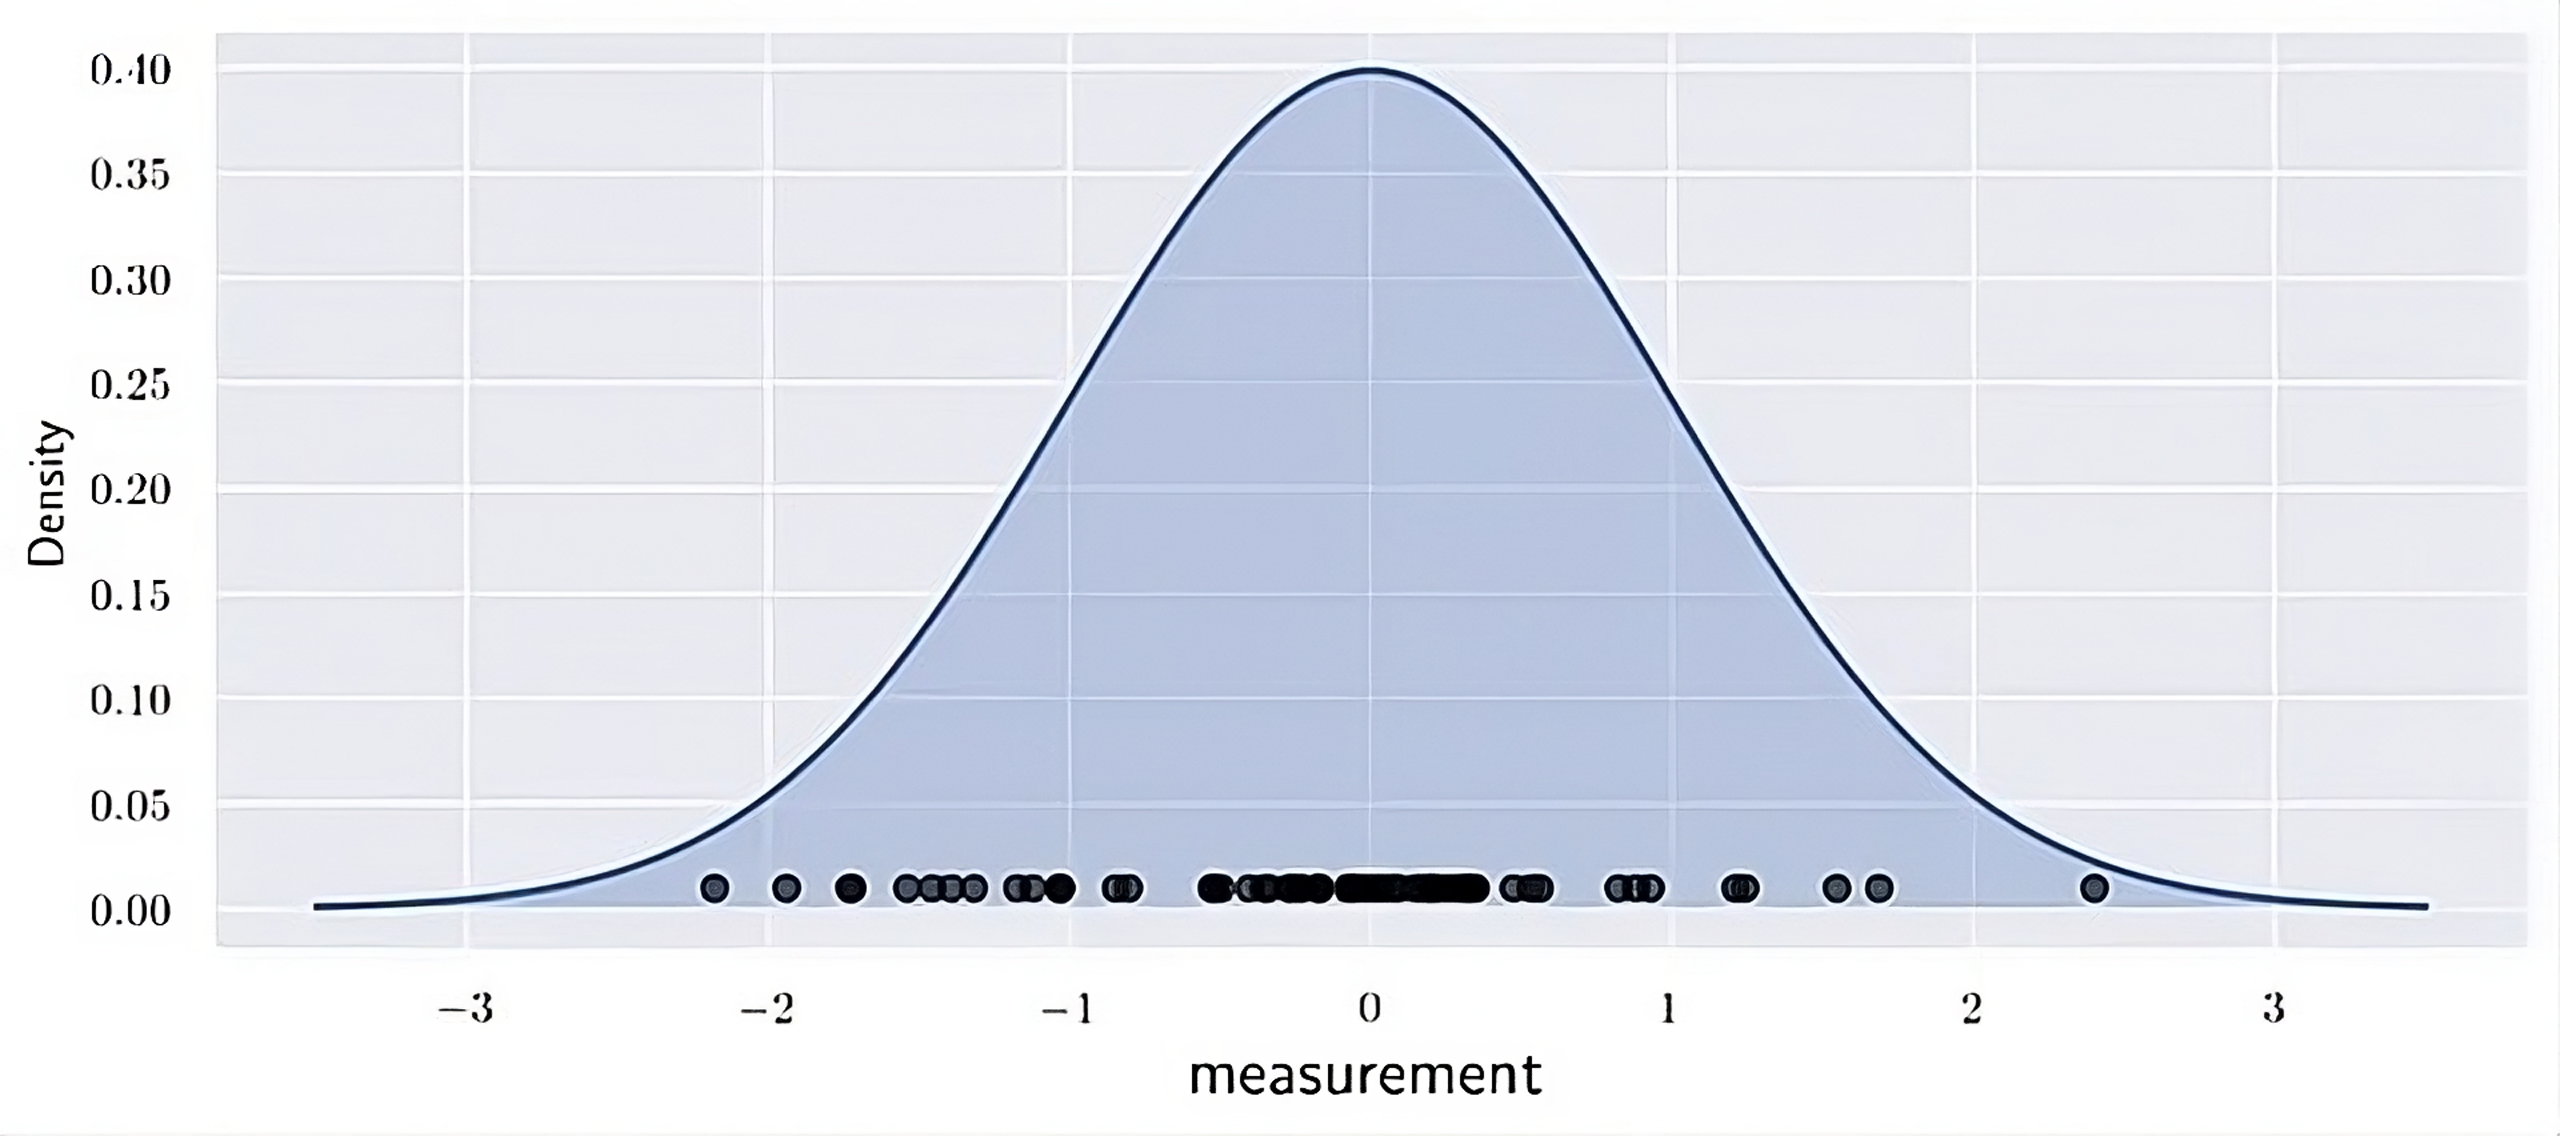
\includegraphics[width=\textwidth]{figChap4/regular-transformed.jpeg}
      \caption{Regular.}
      \label{fig:reg}
  \end{subfigure}  
  \begin{subfigure}[b]{1\textwidth}
      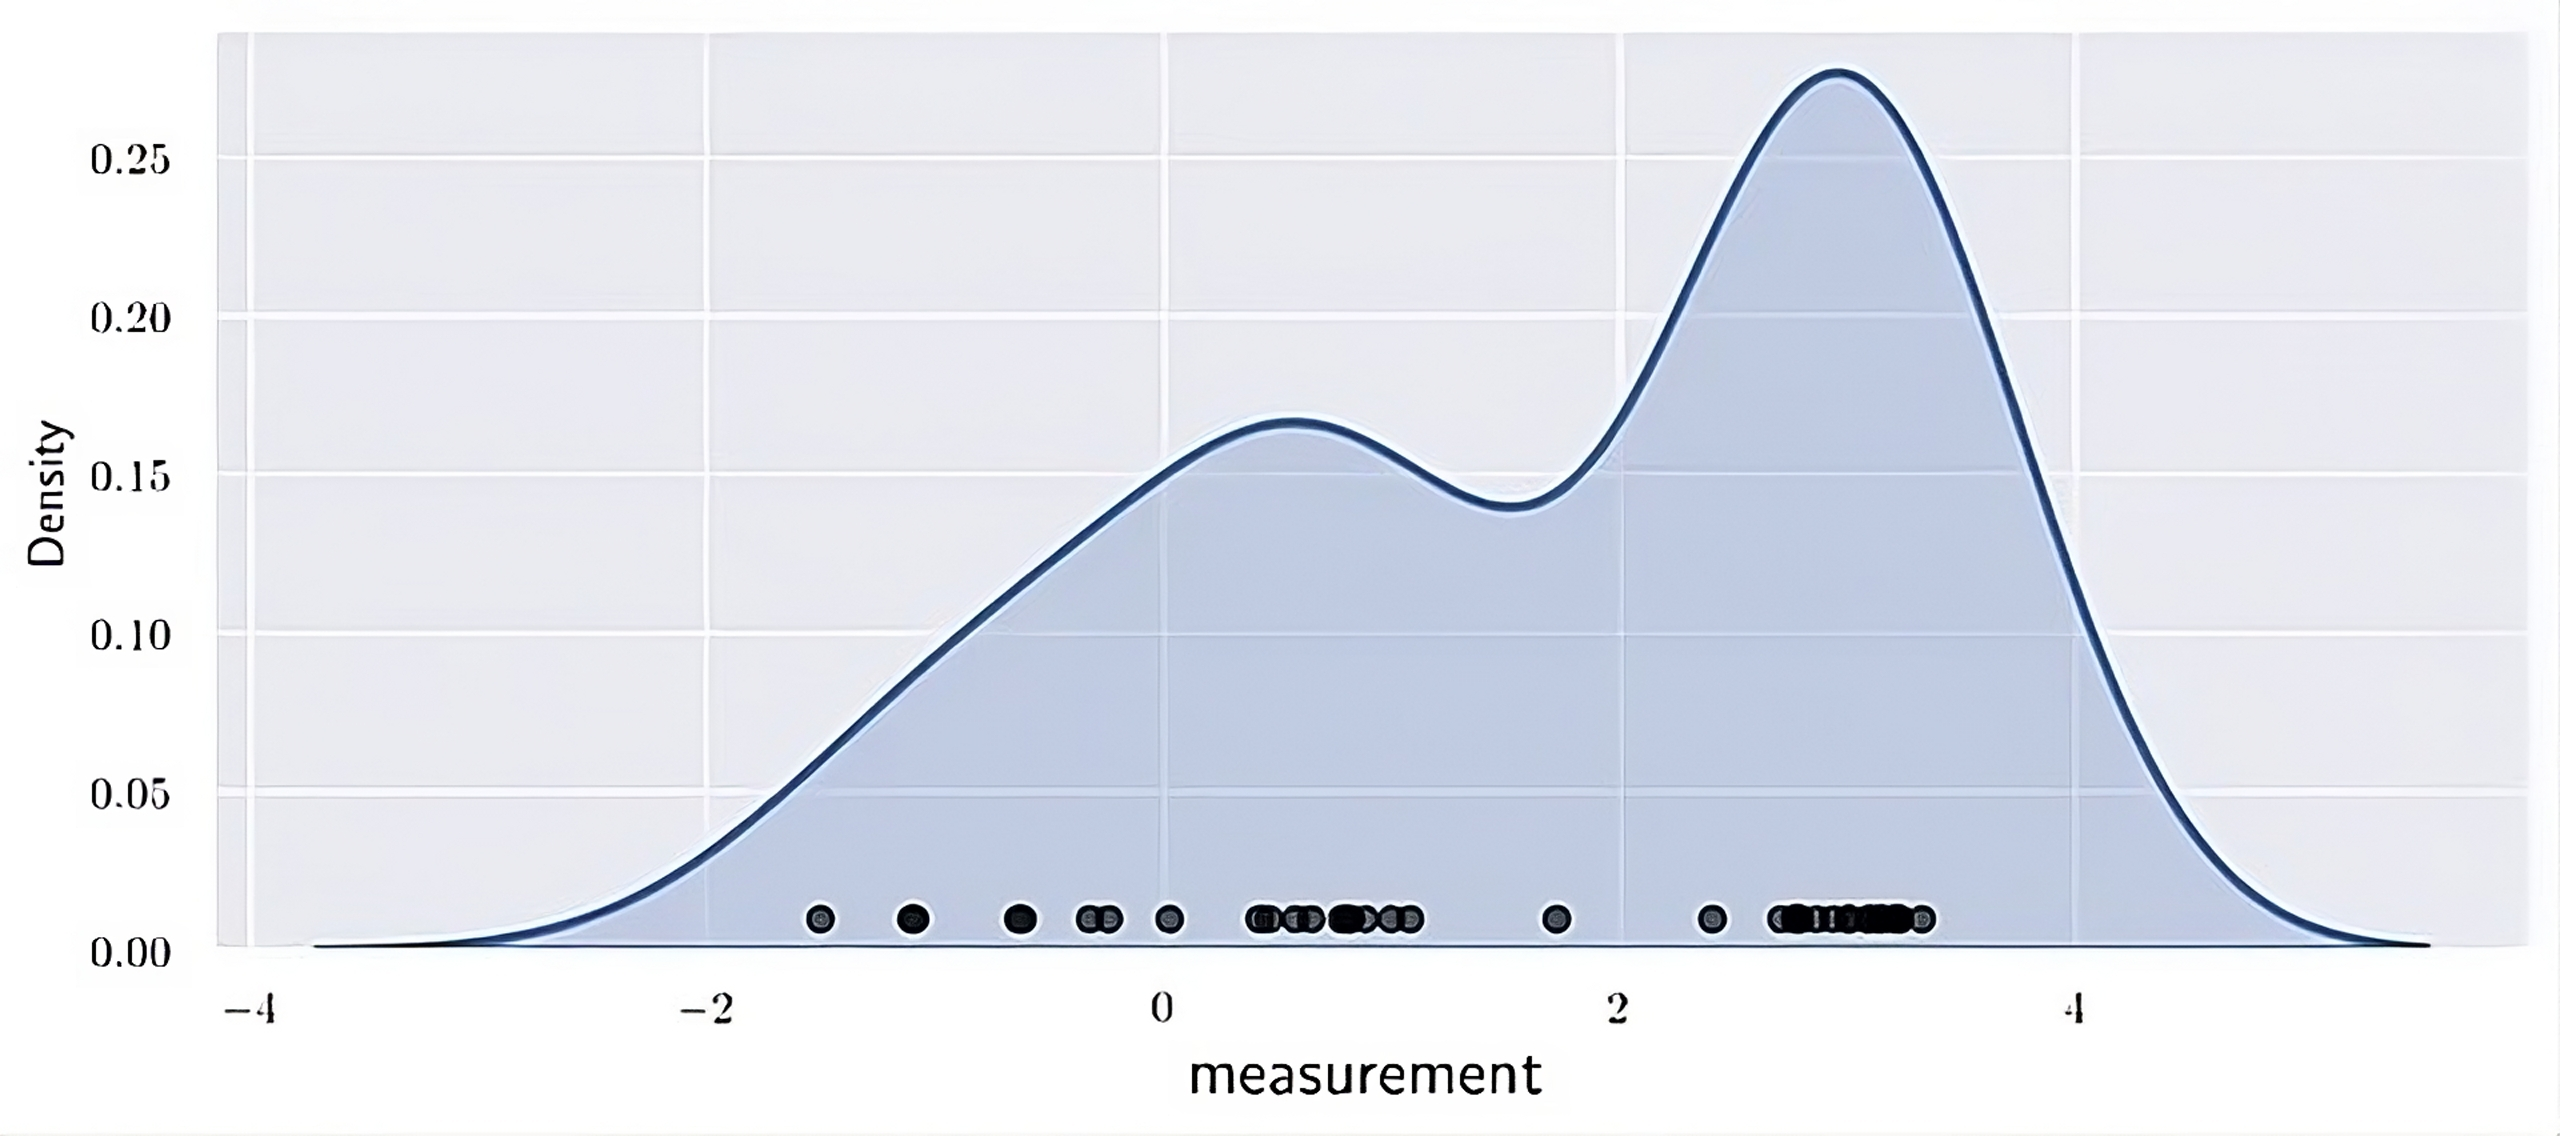
\includegraphics[width=\textwidth]{figChap4/irregular-transformed.jpeg}
      \caption{Irregular.}
      \label{fig:irreg}
  \end{subfigure}
  \caption{One-dimensional example of regular \ref{fig:reg} and irregular \ref{fig:irreg} 
  data distribution.
  Images courtesy of~\cite{Jaroslaw2023KDEexplain}.}
  \label{fig:DataDistribution}
\end{figure}
%---------------------------------------------------------------------------------
In such cases, 
Kernel Density Estimator is employed to approximate the underlying distribution of the data. 
The Kernel Density Estimator \( \hat{f}_\mathcal{X}(x) \) 
for the estimation of the density value at point \( x \) is defined as:
\[ \hat{f}_\mathcal{X}(x) = \frac{1}{m} \sum_{i=1}^{m} K \left( x - x_{i} \right), \]
where $m$ is a number of points $x_i$ in respective dataset $\mathcal{X}_\text{free}$ or $\mathcal{X}_\text{obs}$ and
\( K(x) \) is the Gaussian Kernel function~\cite{Jaroslaw2023KDEmultidimensional}, represented as follows:
\[
K(x) = (2\pi)^{-\frac{d}{2}} \cdot \det(\textbf{H})^{-\frac{1}{2}} \cdot e^{-\frac{1}{2} x^T H^{-1} x},
\]
where \( x \) represents the input vector, 
with a dimension of the input space \( d \), 
\( \textbf{H} \) denotes the bandwidth matrix,
\((2\pi)^{-\frac{d}{2}}\) is a normalization constant.
Matrix \( \textbf{H} \) serves as a covariance matrix and 
acts as a user-defined parameter influencing the kernel function. 
When \( d = 2 \), it corresponds to a bivariate case. 
For instance, in a 2D configuration space, as depicted in Figure \ref{fig:GKDEmaze}, 
the input vector \( x \) comprises two coordinates of the point: \( x = [x_1, x_2] \), and 
the bandwidth matrix takes the 
form \( H = \left[ \begin{array}{cc} h_{11} & h_{12} \\ h_{21} & h_{22} \end{array} \right] \). 
Here, \( h_{11} \) and \( h_{22} \) correspond to the variances 
of \( x_1 \) and \( x_2 \) respectively, 
while \( h_{12} = h_{21} \) represents the covariance between \( x_1 \) and \( x_2 \). 
Because of this, the matrix \( \textbf{H} \) is symmetric. 
An illustrative example of kernel estimation in the configuration space depicted 
in Figure \ref{fig:GKDEmaze} can be observed in Figure \ref{fig:GKDEdensity}.
\\[12pt]
%---------------------------------------------------------------------------------
\begin{algorithm}[H]
  \caption{Sample Density}
  \label{alg:sample_density}
  \KwData{$\mathcal{X}_{\text{obs}}$, $\mathcal{X}_{\text{free}}$}
  \KwResult{Predicted sampled point $x$}
  \vspace{0.1cm}
  \hrule
  \vspace{0.2cm}
  $\gamma_{\text{free}} \gets 0$\;
  $\gamma_{\text{obs}} \gets 1$\; 
  \While{$\gamma_{\text{free}} < \gamma_{\text{obs}}$}{
    $x_{\text{rand}} \gets$ RandomConfiguration()\;
    $P_{\text{free}} \gets \frac{|\mathcal{X}_{\text{free}}|}{|\mathcal{X}_{\text{free}}| + |\mathcal{X}_{\text{obs}}|}$\;
    $P_{\text{obs}} \gets 1 - P_{\text{free}}$\;
    $b_{\text{free}} \gets$ DensityEstimator($x_{\text{rand}}$, $\mathcal{X}_{\text{free}}$)\;
    $b_{\text{obs}} \gets$ DensityEstimator($x_{\text{rand}}$, $\mathcal{X}_{\text{obs}}$)\;
    $\gamma_{\text{free}} \gets b_{\text{free}} \cdot P_{\text{free}}$\;
    $\gamma_{\text{obs}} \gets b_{\text{obs}} \cdot P_{\text{obs}}$\; 
  }
  $x \gets x_{\text{rand}}$\;
  \Return $x$\;
\end{algorithm} 
%---------------------------------------------------------------------------------
\vspace{1em}
\noindent Now, leveraging our density estimator, let us proceed to Bayesian classifier.
Firstly, it is necessary to introduce Bayes' theorem, which is formulated as follows:
\[
  P(A|B) = \frac{P(B|A) \cdot P(A)}{P(B)}.
\]
In this context, 
the aim is to determine the probability of a point \( x \) belonging to a particular space,
denoted by \( P(y|x) \). 
Our Kernel Density Estimator, on the other hand, represents \( P(x|y) \), 
which is the probability distribution of points \( x \) given a specific space \( y \).
As previously mentioned, the training set was divided into 
two datasets: \( \mathcal{X}_\text{free} \) and \( \mathcal{X}_\text{obs} \). 
These datasets were utilized to determine \( P(y) \) for each respective space.
So now our Bayesian theorem looks like this:
\[
  P(y|x) = \frac{P(x|y) \cdot P(y)}{P(x)},
\]
where
\[ P(x|y=1) = \hat{f}_{\mathcal{X}_{\text{obs}}}(x) = \frac{1}{|\mathcal{X}_{\text{obs}}|} \sum_{x' \in \mathcal{X}_{\text{obs}}} K \left( x - x' \right); \]
\[ P(x|y=0) = \hat{f}_{\mathcal{X}_{\text{free}}}(x) = \frac{1}{|\mathcal{X}_{\text{free}}|} \sum_{x' \in \mathcal{X}_{\text{free}}} K \left( x - x' \right); \]
\[ P(y=1) = \frac{|\mathcal{X}_{\text{obs}}|}{|\mathcal{X}_{\text{obs}}|+|\mathcal{X}_{\text{free}}|};\enspace
P(y=0) = \frac{|\mathcal{X}_{\text{free}}|}{|\mathcal{X}_{\text{obs}}|+|\mathcal{X}_{\text{free}}|};\]
\[|\mathcal{X}_{\text{obs}}| \text{ denotes the number of points contained within the } \mathcal{X}_{\text{obs}} \text{ dataset};\]
\[|\mathcal{X}_{\text{free}}| \text{ denotes the number of points contained within the } \mathcal{X}_{\text{free}} \text{ dataset};\]
\[\text{Regarding } P(x), \text{ further discussion will follow}.\]
Now, the Bayesian decision rule can be formulated. 
This rule will be represented as a function \( f: \mathcal{X} \mapsto \{0,1\} \), 
which will predict the label of the given point:
\[ f(x) = 
  \begin{cases}
  0 & \text{if } \gamma_{\text{free}}(x) \geq \gamma_{\text{obs}}(x), \\
  1 & \text{otherwise,}
  \end{cases} 
\]
where 
\[\gamma_{\text{free}}(x) = P(y=0|x);\enspace \gamma_{\text{obs}}(x) = P(y=1|x).\]

In this decision rule, where $\gamma_{\text{free}}(x) \geq \gamma_{\text{obs}}(x)$, 
it's evident that the computation of $P(x)$ is not necessarily required.
\\[12pt]
The proposed solution is outlined in Algorithm \ref{alg:sample_density}: Sample Density. 
Default parameters for $\gamma_{\text{free}}$ and $\gamma_{\text{obs}}$ are defined 
at Line 1 and Line 2, 
where $\gamma_{\text{free}}$ should be less than $\gamma_{\text{obs}}$. 
The main process occurs within a while loop at Line 3-10. 
The condition in this loop is inverted compare to our decision rule 
because the goal is to exit the loop when this condition is met. 
Inside this loop, a random point is generated at each iteration. 
\\[12pt]
For each random point, the probability of belonging to each space 
is computed as explained in this section.
Subsequently, the point predicted to be in the $C_{\text{free}}$ space is returned.
Now, let us explore how this method can be integrated with sampled-based methods.
% In such cases, Kernel Density Estimator is employed to approximate the underlying 
% distribution of the data. 
% In this work, the Gaussian Kernel function was utilized, represented as follows:
% \[
% K(x) = (2\pi)^{-\frac{d}{2}} \cdot \det(H)^{-\frac{1}{2}} \cdot e^{-\frac{1}{2} x^T H^{-1} x},
% \]
% where \( x \) represents the input vector, 
% with a dimension of the input space \( d \), 
% \( H \) denotes the bandwidth matrix, \((2\pi)^{-\frac{d}{2}}\) is a normalization constant,
% and \( d \) signifies the dimensionality of the input space.
% The Kernel Density Estimator \( \hat{f}_X(x) \) for 
% the estimation of the density value \( f_X(x) \) at point \( x \) is defined as:
% \[ \hat{f}_\mathcal{X}(x) = \frac{1}{m} \sum_{i=1}^{m} K \left( x - x^{(i)} \right) \]


%---------------------------------------------------------------------------------
%---------------------------------------------------------------------------------
\begin{figure}[!ht]
  \centering 
    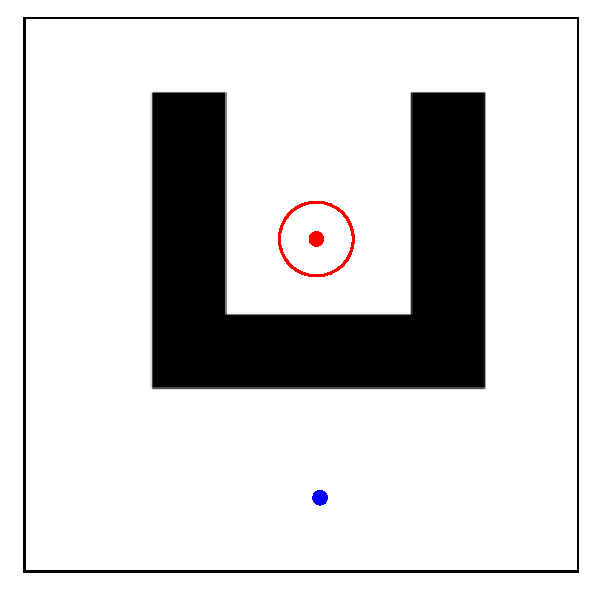
\includegraphics[width=0.5\textwidth]{figChap4/SimpleMaze.eps} 
  \caption{An example of the 2D $\mathcal{C}$-space.}
  \label{fig:GKDEmaze}
\end{figure}
%---------------------------------------------------------------------------------

\begin{figure}[!ht]
  \centering 
  \begin{subfigure}[b]{1\textwidth}
      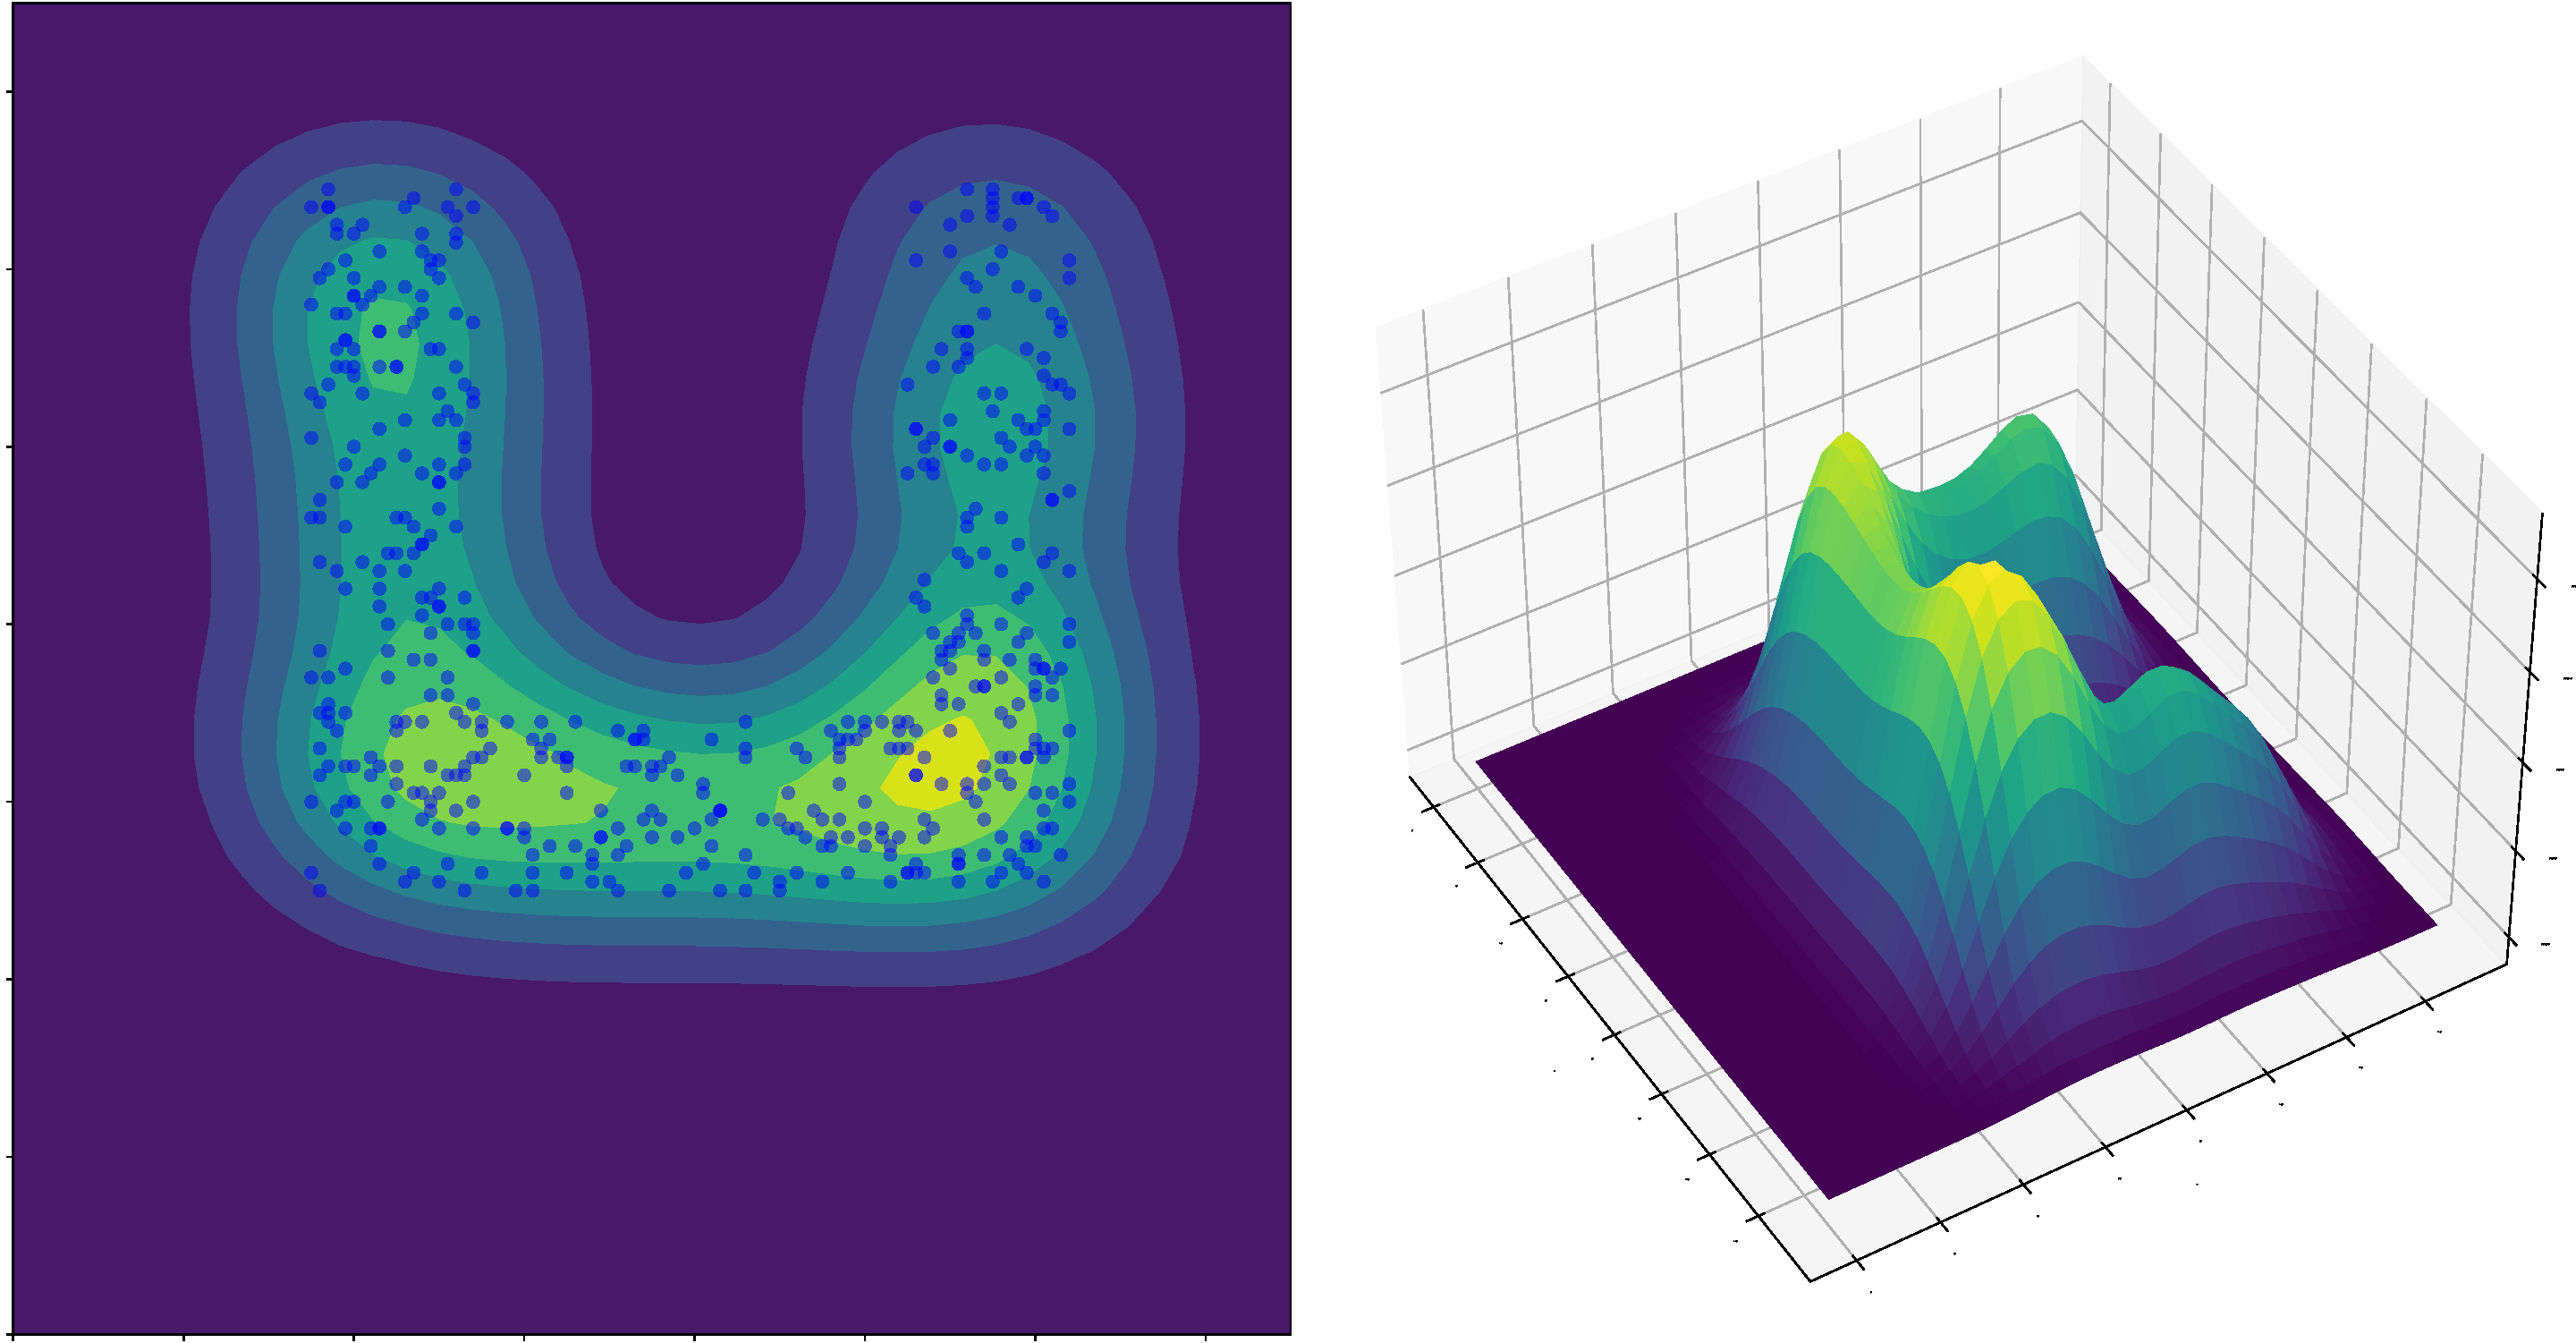
\includegraphics[width=\textwidth]{figChap4/GKDE_obsU.pdf}
      \caption{Obstacle density.}
      \label{fig:GKDEobstacleSpace}
  \end{subfigure}  
  \begin{subfigure}[b]{1\textwidth}
      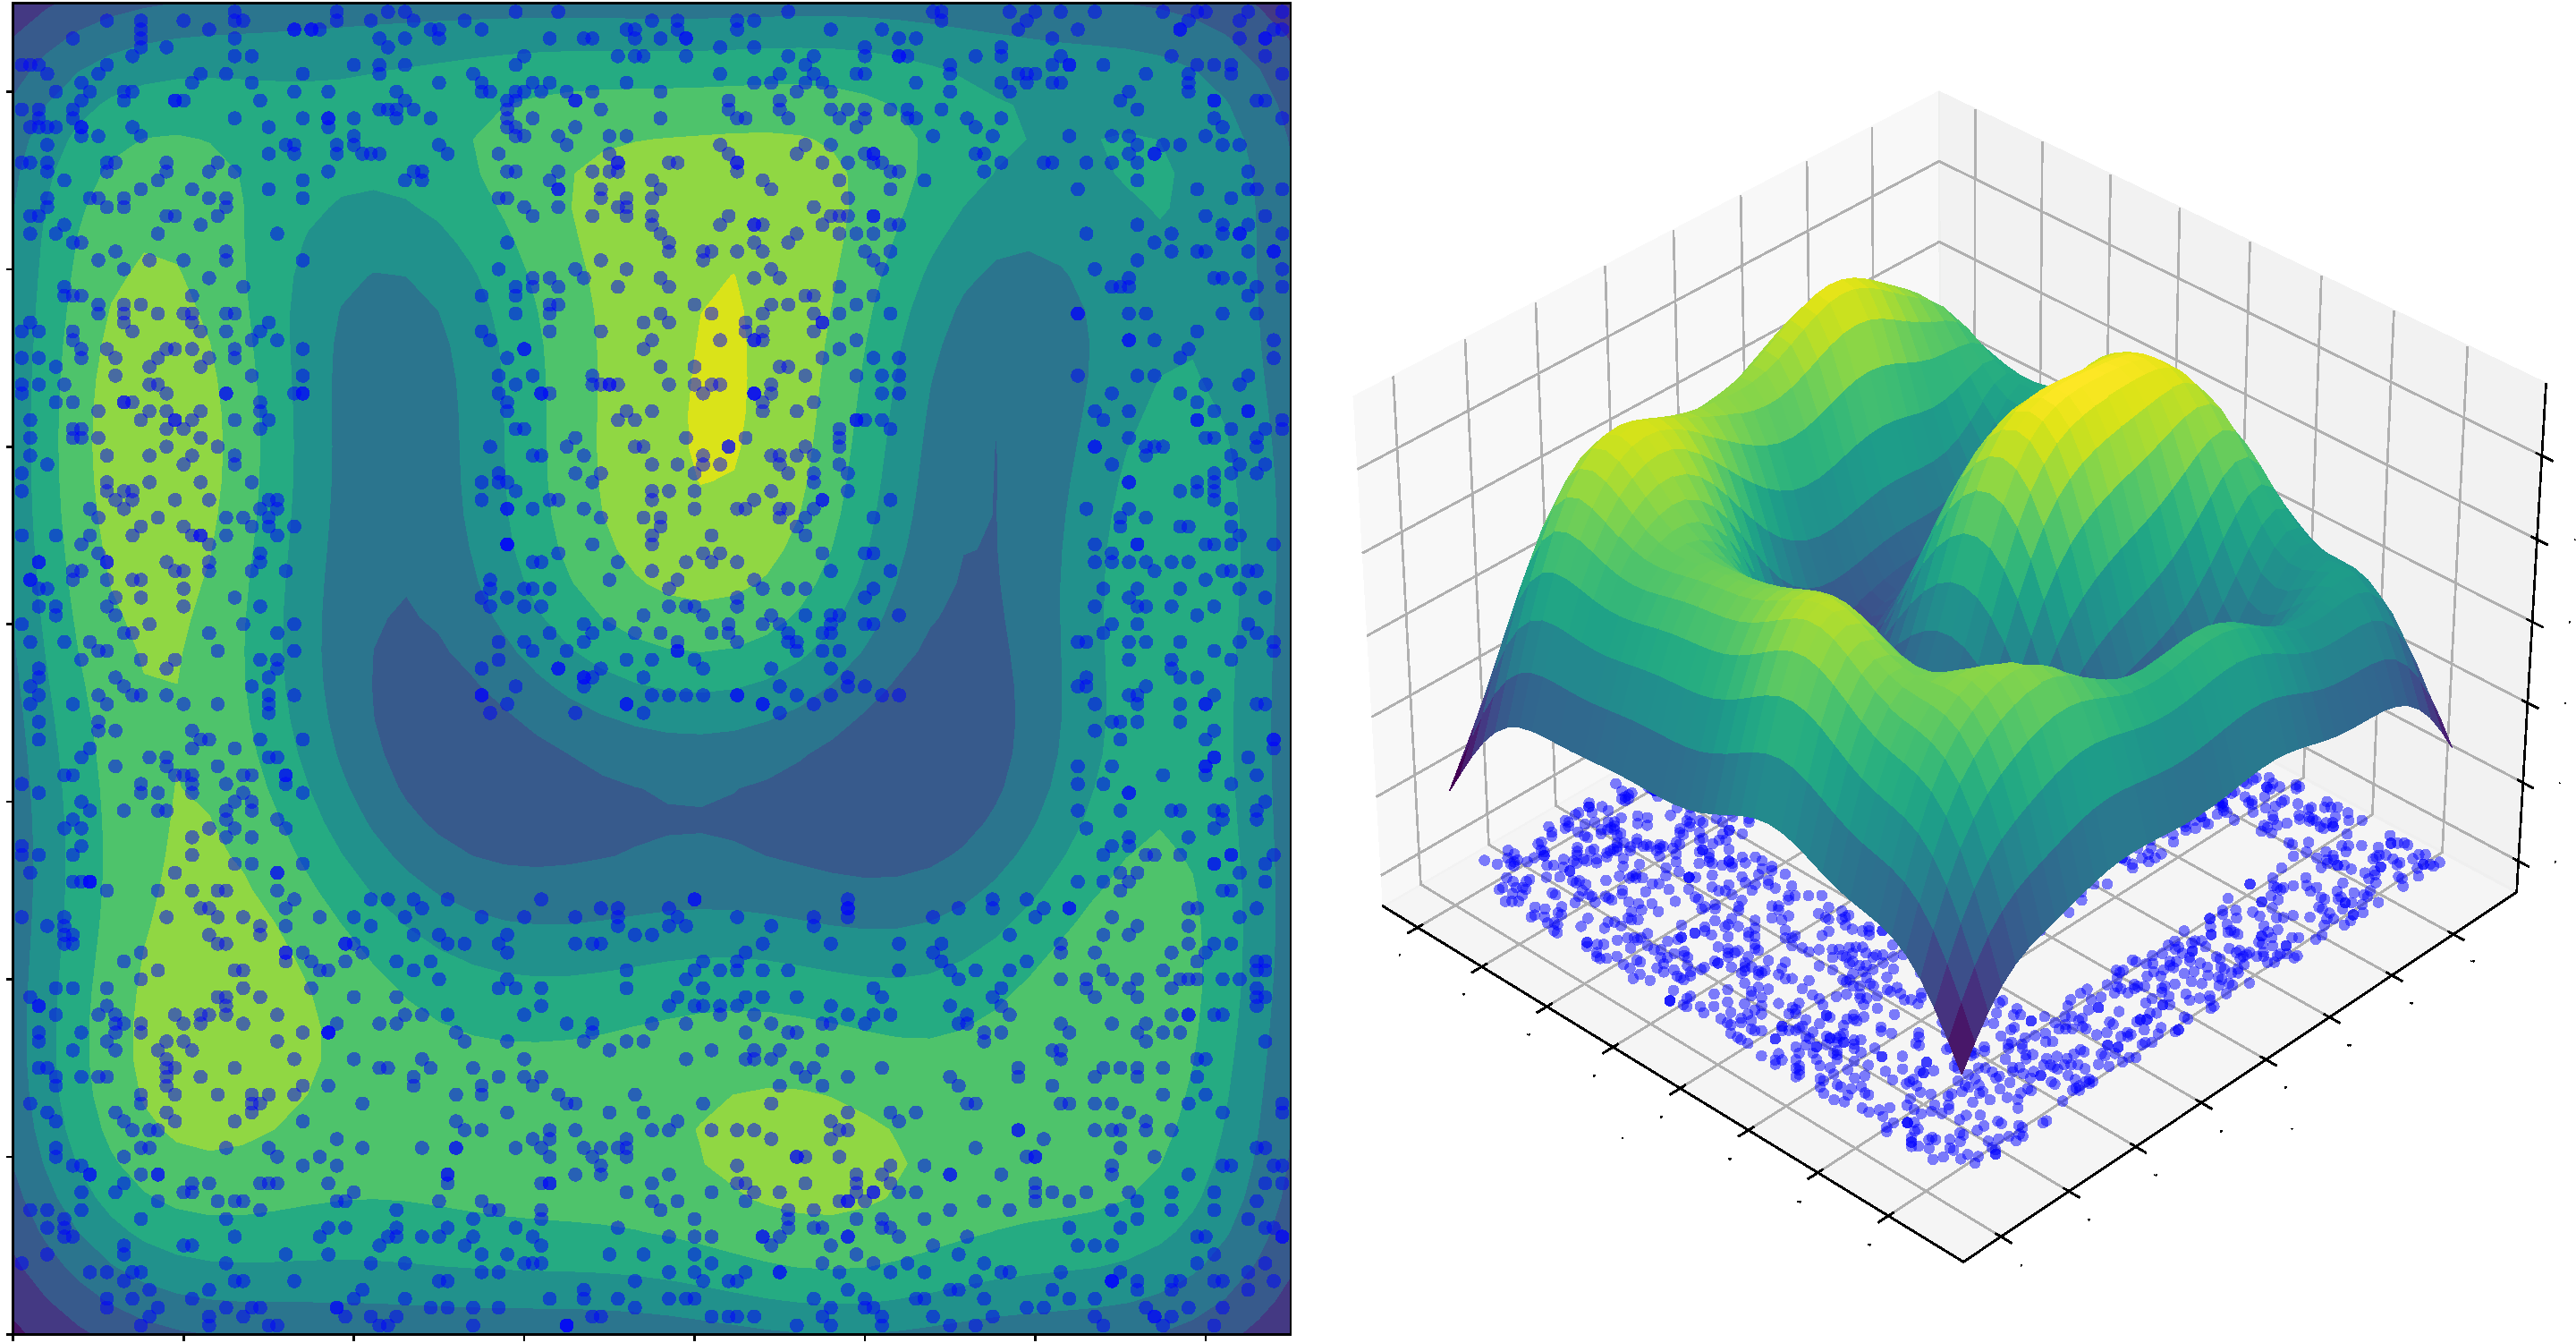
\includegraphics[width=\textwidth]{figChap4/GKDE_freeU.pdf}
      \caption{Obstacle-free density.}
      \label{fig:GKDEfreeSpace}
  \end{subfigure}
  \caption{An example of density estimation with Gaussian Kernel function 
  of the $\mathcal{C}$-space in Figure \ref{fig:GKDEmaze}. 
  Circles represent randomly generated points in the $\mathcal{C}$-space. 
  In Figure \ref{fig:GKDEobstacleSpace}, the density estimation of the 
  obstacle space can be seen. 
  Figure \ref{fig:GKDEfreeSpace} illustrates the density estimation of the free space. 
  The higher the graph, 
  the higher the density, indicating a higher probability for points to be in respective space.}
  \label{fig:GKDEdensity}
\end{figure}

%---------------------------------------------------------------------------------
%---------------------------------------------------------------------------------
\section{Integration to the RRT* algorithm}

The proposed solution is designed to be compatible with any sampling-based method 
that employs single configuration generation to explore the configuration space 
in a single iteration. 
In this implementation, RRT* was specifically chosen for its ability to converge 
efficiently towards an optimal solution while effectively exploring the configuration space. 
%---------------------------------------------------------------------------------
\begin{figure}[!ht]
  \centering 
  \begin{subfigure}[b]{0.45\textwidth}
      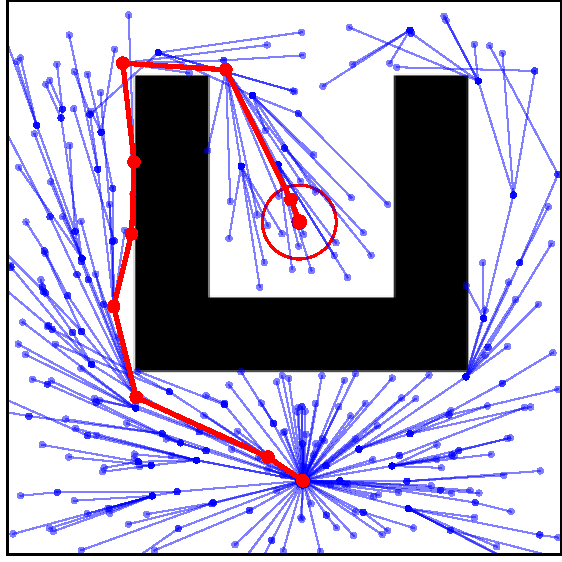
\includegraphics[width=\textwidth]{figChap4/RRTstar_maze216.0.pdf}
      \caption{RRT*.}
      \label{fig:rrtstar_maze}
  \end{subfigure}  
  \begin{subfigure}[b]{0.45\textwidth}
      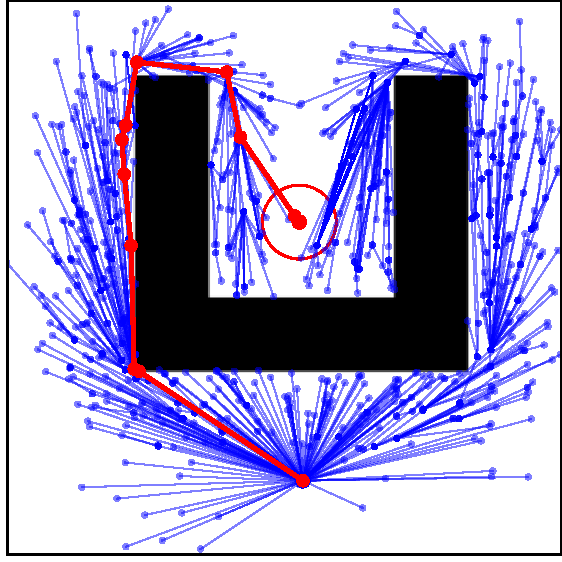
\includegraphics[width=\textwidth]{figChap4/RRTstarML_maze206.0.pdf}
      \caption{Improven RRT*.}
      \label{fig:rrtstarML_maze}
  \end{subfigure}
  \caption{
    Both algorithms, RRT* \ref{fig:rrtstar_maze} and 
    the improved RRT* using machine learning \ref{fig:rrtstarML_maze} methods, are presented, 
    each consisting of 1000 iterations. 
    It is evident that the improved RRT* efficiently explores the configuration space and 
    eventually finds a path to the goal with the lowest cost of 206 u.d.(units of dimension), 
    compared to RRT*, which finds a path to the goal with a cost of 216 u.d.. 
    Additionally, despite both algorithms having the same number of iterations, 
    the improved RRT* exhibits a higher number of collision-free paths found. 
    This difference arises from the strategy of sampling points in the $\mathcal{C}$-space, 
    which increases the probability of finding a collision-free path after each iteration.}
  \label{fig:RRTstar_vs_RRTstarML}
\end{figure}
%---------------------------------------------------------------------------------
\begin{figure}[!ht]
  \centering 
  \begin{subfigure}[b]{0.45\textwidth}
      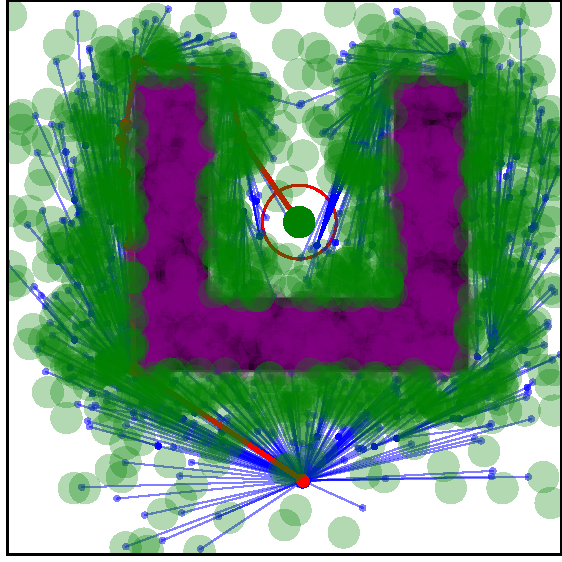
\includegraphics[width=\textwidth]{figChap4/RRTstarML_learning206.0.pdf}
      \caption{Learning the $\mathcal{C}$-space.}
      \label{fig:rrtstarML_learning}
  \end{subfigure}  
  \begin{subfigure}[b]{0.45\textwidth}
      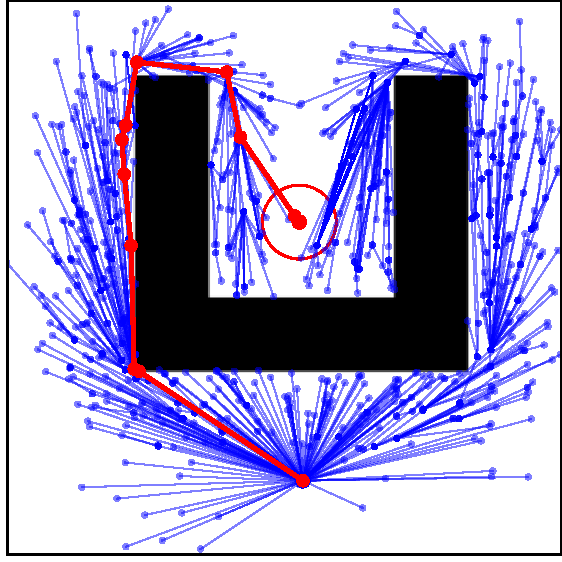
\includegraphics[width=\textwidth]{figChap4/RRTstarML_maze206.0.pdf}
      \caption{Improven RRT*.}
      % \label{fig:rrtstarML_maze}
  \end{subfigure}
  \caption{In Figure \ref{fig:rrtstarML_learning}, 
  the information about the $\mathcal{C}$-space can be seen. 
  The purple color represents the \( \mathcal{X}_{\text{obs}} \) dataset, 
  while the green color represents the \( \mathcal{X}_{\text{free}} \) dataset. 
  Utilizing these datasets, the algorithm learns the $\mathcal{C}$-space.}
  \label{fig:LearningConfigSpace}
\end{figure}
%---------------------------------------------------------------------------------
\\[12pt]
The integration approach relies on a specific function for sampling predicted points,
rather than utilizing random sampling. 
This function is outlined in Algorithm \ref{alg:ml_sample}. 
Within the while loop, 
point predicted by the function $f$ to be in the $\mathcal{C}_{\text{free}}$ are generated. 
After each iteration, 
the algorithm verifies if this point indeed lies inside $\mathcal{C}_{\text{free}}$, 
and upon finding such a point, it is returned. 
If a point lies within the $\mathcal{C}_{\text{obs}}$ space, 
it is added to the $\mathcal{X}_{\text{obs}}$ dataset.
Otherwise, it is added to the $\mathcal{X}_{\text{free}}$ dataset.
This function effectively replaces the random configuration generation step 
in Algorithm \ref{alg:rrt_star}, Line 3, thus demonstrating integration with the RRT* algorithm.
\\[12pt] 
%---------------------------------------------------------------------------------
\begin{algorithm}[H]
  \caption{Sample}
  \label{alg:ml_sample}
  \KwData{$\mathcal{X}_{\text{obs}}$, $\mathcal{X}_{\text{free}}$}
  \KwResult{Sampled point $x$}
  \vspace{0.1cm}
  \hrule
  \vspace{0.2cm}
  $x \gets$ Sample Density($\mathcal{X}_{\text{obs}}$, $\mathcal{X}_{\text{free}}$); \hfill // Algorithm \ref{alg:sample_density}\; 
  \While{OnObstacle($x$)}{ 
    $\mathcal{X}_{\text{obs}} \gets \mathcal{X}_{\text{obs}} \cup$ \{x\}\;
    $x \gets$ Sample Density($\mathcal{X}_{\text{obs}}$, $\mathcal{X}_{\text{free}}$);\hfill // Algorithm \ref{alg:sample_density}\; 
  }
  $\mathcal{X}_{\text{free}} \gets \mathcal{X}_{\text{free}} \cup$ \{x\}\;
  
  \Return $x$\;
\end{algorithm}
%---------------------------------------------------------------------------------
\vspace{1em}
\noindent To demonstrate how this enhancement works, 
in Figure \ref{fig:RRTstar_vs_RRTstarML} can be seen 
the expansion of RRT* with enhanced RRT* using 
machine learning, which explores $\mathcal{C}$-space. 
Figure \ref{fig:LearningConfigSpace} illustrates 
the learning process of the $\mathcal{C}$-space by our enhanced RRT* algorithm.
\\[12pt]
After explaining how the proposed solution was integrated into the RRT*, 
it is crucial to evaluate its effectiveness compared to other planners. 
Chapter \ref{chap:Result} provides further insights into this comparative analysis.
%---------------------------------------------------------------------------------
%---------------------------------------------------------------------------------
\section{Extension of the machine learning method to 3D and 6D configuration spaces}
In this problem, the robot is represented as a polygon. 
To describe the position of the robot in space, three coordinates are utilized: 
two for its position in $\mathcal{C}$-space and 
a third one for its rotation angle. 
The position of the robot is defined as its center of mass.
The main difference from the implementation in 2D $\mathcal{C}$-space is that 
the procedure for checking whether a point is inside the $\mathcal{C}_\text{obs}$,
as shown in Algorithm \ref{alg:ml_sample} Line 2,
is replaced by a function that checks if 
at least one point of robot lies inside the $\mathcal{C}_\text{obs}$. 
Also, verifying whether the path is obstacle-free, 
it is essential to ensure that 
the robot does not collide with obstacles while moving along the path.
To address this, 
linear interpolation between two points is utilized 
to detect potential collisions between the robot and obstacles along the path.
The linear interpolation formula \[ q(s) = (1 - s) \cdot q_{\text{near}} + s \cdot q_{\text{new}},\enspace s \in [0,1], \] 
defines the points along the line segment connecting \( q_{\text{near}} \) and \( q_{\text{new}} \).
Consequently, the $\mathcal{X}_\text{obs}$ space is not always represented just by the 
area of the obstacle, but also includes points where the robot intersects 
with the obstacle. 
An example can be seen in Figure \ref{fig:LearningConfigSpace2D}.
\\[12pt]
Similarly as in 2D $\mathcal{C}$-space, 
the improved version of RRT* demonstrates better performance 
in finding optimal paths \ref{fig:RRTstar2D_vs_RRTstarML2D}. 
%---------------------------------------------------------------------------------
\begin{figure}[!ht]
  \centering 
  \begin{subfigure}[b]{0.45\textwidth}
      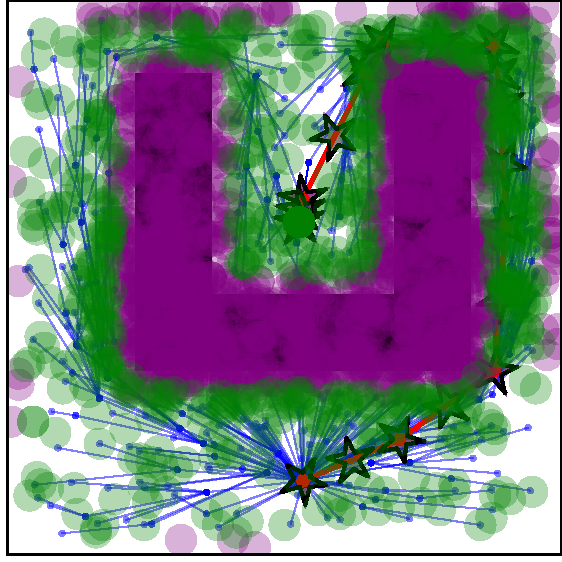
\includegraphics[width=\textwidth]{figChap4/RRTstar2DML_learning237.2.pdf}
      \caption{Learning the $\mathcal{C}$-space.}
      \label{fig:rrtstarML2D_learning}
  \end{subfigure}  
  \begin{subfigure}[b]{0.45\textwidth}
      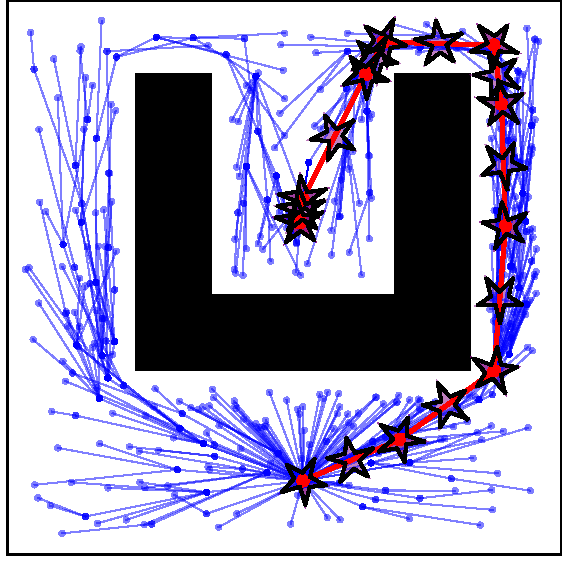
\includegraphics[width=\textwidth]{figChap4/RRTstar2DML_maze237.2.pdf}
      \caption{Improven RRT*.}
      % \label{fig:rrtstarML2D_maze}
  \end{subfigure}
  \caption{In Figure \ref{fig:rrtstarML2D_learning}, it can be seen 
  that the $\mathcal{X}_{\text{obs}}$ dataset contains more data points. 
  This is because the purple area contains not only points inside 
  the $\mathcal{C}_{\text{obs}}$,
  but also points where robot, 
  represented as a polygon in the shape of a star, 
  collides with obstacles.}
  \label{fig:LearningConfigSpace2D}
\end{figure}
%---------------------------------------------------------------------------------
\begin{figure}[!ht]
  \centering 
  \begin{subfigure}[b]{0.45\textwidth}
      \includegraphics[width=\textwidth]{figChap4/RRTstar2D_maze241.4.pdf}
      \caption{RRT*.}
      \label{fig:rrtstar2D_maze}
  \end{subfigure}  
  \begin{subfigure}[b]{0.45\textwidth}
      \includegraphics[width=\textwidth]{figChap4/RRTstar2DML_maze237.2.pdf}
      \caption{Improven RRT*.}
      \label{fig:rrtstarML2D_maze}
  \end{subfigure}
  \caption{Both algorithms, 
  RRT* \ref{fig:rrtstar2D_maze} and the improved RRT* using 
  machine learning \ref{fig:rrtstarML2D_maze} methods, 
  are presented, each consisting of 1000 iterations. 
  The improved RRT* finds a path to the goal with 
  the lowest cost of 237.2 u.d. (units of dimension), compared to RRT*, 
  which finds a path to the goal with a cost of 241.4 u.d..}
  \label{fig:RRTstar2D_vs_RRTstarML2D}
\end{figure}
%---------------------------------------------------------------------------------
\\[12pt]
To extend the improved RRT* to 6D $\mathcal{C}$-space, 
such as in the Piano Movers Problem, similar procedures to those in 3D $\mathcal{C}$-space 
need to be followed. 
However, the robot will be represented by a 3D triangle mesh, such as objecct files(.obj). 
These files, readily available from the internet, 
offer a structured representation of objects, 
with each object represented as a set of triangles. 
This triangle representation, similar to a mesh, 
decomposes every object into triangles. 
Additionally, collision detection becomes more complex in this scenario. 
To address this, the RAPID library~\cite{gottschalk1997rapid} can be utilized. 
RAPID (Robust and Accurate Polygon Interference Detection), implemented in C++, 
is a robust tool for collision detection in 3D environments. 
It provides a narrow and user-friendly API (Application Programming Interface) for programmers, 
simplifying the detection of intersections between polygons in various applications such as 
physically based modeling, virtual prototyping, and CAD.  
%---------------------------------------------------------------------------------
%---------------------------------------------------------------------------------
%---------------------------------------------------------------------------------
\chapter{Results and discussion} 
\label{chap:Result} 
Throughout this chapter, 
the performance of the implemented RRT* with machine learning methods, 
denoted as RRT*\_ML in the rest of the text,
will be presented and discussed 
alongside other planners across various configuration spaces. 
In this work, the specification of units of measurement is not necessary 
as the choice of units can vary depending on the preferences or requirements.
\section{Comparison with OMPL}
To assess the effectiveness of the implemented enhanced RRT* algorithm across various scenarios, 
planners from the Open Motion Planning Library (OMPL)~\cite{Ioan2012ompl} 
will serve as benchmarks. 
OMPL is a widely-used library that provides an extensive collection of motion planning algorithms,
making it a valuable resource for comparing and evaluating different planning strategies. 
\\[12pt]
The primary objective of this comparison is to evaluate how integrating 
machine learning methods enhances the performance of the RRT* algorithm. 
Additionally, 
the implemented method will be compared against similar planners that provide 
information about the cost of the path, 
such as RRT$^\#$ (sharp)~\cite{arslan2012rrtsharp}, $\text{RRT}^X$ static~\cite{Otte2015RRTX}, 
and Informed RRT*~\cite{Gammell2018InformedRRTstar}. 
This comparative analysis will offer insights into how our approach 
performs in terms of optimizing path costs compared to these existing algorithms. 
%---------------------------------------------------------------------------------
%---------------------------------------------------------------------------------
\subsection{Planners parameters}
All planners share a common goal bias parameter, \( p_{\text{goal}} = 0.05 \), 
indicating that there is a 5\% probability that a randomly sampled point 
will serve as a goal point. 
While RRT$^\#$ and RRT$^X$ static share similar implementations, 
they diverge in their use of the parameter \( \epsilon \). 
In the case of RRT$^\#$, \( \epsilon \) is set to 0, 
whereas in RRT$^X$ static, it is initially set to 0.01. 
$\epsilon$ representing the minimum
threshold for cost improvement required to rewire the tree
\\[12pt]
Additionally, all OMPL planners start with a rewiring factor of 1.1. 
This factor, applied multiplicatively, 
determines the size of the neighbor ball or the number of neighbors 
considered during tree expansion. 
%---------------------------------------------------------------------------------
\begin{table}[htbp]
  \centering
  \begin{tabular}{|p{3cm}|c|c|}
      \hline
      \textbf{Name} & \textbf{Parameter} & \textbf{Value}\\
      \hline
      Goal bias       & $p_{goal}$ & 0.05 \\
      Epsilon         & $\epsilon$ & 0.01 \\
      Rewire Factor   & $k$        & 1.1  \\
      Rewiring radius & $r$        & 40   \\
      Step size       & $s$        & 10   \\
      % Add more rows as needed
      \hline
  \end{tabular}
  \caption{Planners parameters.}
  \label{tab:params}
\end{table}
%--------------------------------------------------------------------------------- 
\\
In the implementation of RRT*\_ML, 
the rewiring radius is set to 40 and the step size to 10. 
The rewiring radius represents the radius within which nearest neighbor 
searches are conducted, 
while the step size represents the maximum length of a path segment.
\\[12pt]
The parameters for RRT*\_ML were manually tuned, 
potentially resulting in suboptimal solutions. 
In certain scenarios, a larger or smaller rewiring radius or step size might be more beneficial. 
As a consequence, 
the OMPL implementation may outperform the custom Python implementation in terms of speed. 
\\[12pt]
All parameters are listed in Table \ref{tab:params}.
%--------------------------------------------------------------------------------- 
%--------------------------------------------------------------------------------- 
\subsection{Cost convergence analysis}
This subsection will present a comparative analysis of the RRT*\_ML method with OMPL planners, 
with a focus on their convergence during iterations.
To enhance visibility and emphasize changes, the graphs will be scaled. 
Therefore, the Y-axis will be adjusted to start 
at a value just below the convergence line of the graph, 
ensuring larger and clearer graph representation (Figure \ref{fig:graph_scale}).
In all configuration spaces discussed in this subsection, 
the robot is represented by a point. 
A green circle indicates the start configuration, 
a red area signifies the goal configuration space, 
and a red point denotes the goal configuration. 
Black areas represent obstacles.
%---------------------------------------------------------------------------------
\begin{figure}[!ht]
  \centering 
  \begin{subfigure}[b]{0.49\textwidth}
    \includegraphics[width=\textwidth]{figChap5/graph_U_20pt_ticks_big.pdf}
    \caption{Original unscaled graph.}
    % \label{fig:maze_E_Cspace} 
  \end{subfigure}  
  \begin{subfigure}[b]{0.49\textwidth}
    \includegraphics[width=\textwidth]{figChap5/graph_U_20pt_ticks.pdf}  
    \caption{Scaled graph.}
    % \label{fig:maze_U_graphs}
  \end{subfigure} 
  \caption{To enhance visualization of the graphs, all will be scaled to depict changes more clearly. 
  Consequently, the cost axes will not necessarily start at zero.}
  \label{fig:graph_scale}
\end{figure}
%---------------------------------------------------------------------------------
\\
Figures \ref{fig:maze_U}, \ref{fig:maze_E}, \ref{fig:maze_clutter}, \ref{fig:maze_narrow} 
depict the configuration spaces and convergence graphs of each planner. 
All tests were conducted up to a point where the graphs showed minimal change.
Path costs were computed the same way across all planners, as the path length.
\\[12pt]
In Figure \ref{fig:maze_U}, 
a simple configuration space, previously discussed, is shown. 
The implemented machine learning method, denoted as RRT*\_ML, 
notably converges faster to the optimal solution compared to RRT*. 
Other planners, while slightly slower, also find solutions. 
However, the performance of the implemented machine learning method surpasses 
that of the other planners in this scenario.
\\[12pt]
Figure \ref{fig:maze_E} illustrates a simple example of narrow passages. 
The implemented method discovers a solution slightly earlier than other planners, 
although its performance becomes comparable to RRT* after 2000 iterations.
%---------------------------------------------------------------------------------
\begin{figure}[!ht]
  \centering 
  \begin{subfigure}[b]{0.48\textwidth}
    \includegraphics[width=\textwidth]{figChap5/graph_U_20pt_ticks.pdf}  
    \caption{Graph.}
    \label{fig:maze_U_graphs}
  \end{subfigure}
  \begin{subfigure}[b]{0.49\textwidth}
      \includegraphics[width=\textwidth]{figChap5/Maze_U_ticks.pdf}
      \caption{$\mathcal{C}$-space.}
      \label{fig:maze_U_Cspace} 
  \end{subfigure}  
  \caption{$\mathcal{C}$-space with small $\mathcal{C}_\text{obs} $ \ref{fig:maze_U_Cspace} and 
  corresponding convergence graphs \ref{fig:maze_U_graphs} of selected planners.}
  \label{fig:maze_U}
\end{figure}
%---------------------------------------------------------------------------------
\begin{figure}[!ht]
  \centering 
  \begin{subfigure}[b]{0.48\textwidth}
    \includegraphics[width=\textwidth]{figChap5/graph_E_20pt_ticks.pdf}  
    \caption{Graph.}
    \label{fig:maze_E_graphs}
  \end{subfigure}
  \begin{subfigure}[b]{0.49\textwidth}
      \includegraphics[width=\textwidth]{figChap5/Maze_E_ticks.pdf}
      \caption{$\mathcal{C}$-space.}
      \label{fig:maze_E_Cspace} 
  \end{subfigure}   
  \caption{$\mathcal{C}$-space with narrow passages \ref{fig:maze_E_Cspace} and 
  corresponding convergence graphs \ref{fig:maze_E_graphs} of selected planners.}
  \label{fig:maze_E}
\end{figure}
%---------------------------------------------------------------------------------
\begin{figure}[!ht]
  \centering 
  \begin{subfigure}[b]{0.48\textwidth}
    \includegraphics[width=\textwidth]{figChap5/graph_clutter_20pt_ticks.pdf}  
    \caption{Graph.}
    \label{fig:maze_clutter_graphs}
  \end{subfigure}
  \begin{subfigure}[b]{0.49\textwidth}
      \includegraphics[width=\textwidth]{figChap5/Maze_clutter_ticks.pdf}
      \caption{$\mathcal{C}$-space.}
      \label{fig:maze_clutter_Cspace} 
  \end{subfigure}   
  \caption{Cluttered $\mathcal{C}$-space \ref{fig:maze_clutter_Cspace} and 
  corresponding convergence graphs \ref{fig:maze_E_graphs} of selected planners.}
  \label{fig:maze_clutter}
\end{figure}
%---------------------------------------------------------------------------------
\begin{figure}[!ht]
  \centering 
  \begin{subfigure}[b]{0.48\textwidth}
    \includegraphics[width=\textwidth]{figChap5/graph_narrow_20pt_ticks.pdf}  
    \caption{Graph.}
    \label{fig:maze_narrow_graphs}
  \end{subfigure}
  \begin{subfigure}[b]{0.49\textwidth}
      \includegraphics[width=\textwidth]{figChap5/Maze_narrow_ticks.pdf}
      \caption{$\mathcal{C}$-space.}
      \label{fig:maze_narrow_Cspace}  
  \end{subfigure}  
  \caption{Difficult  $\mathcal{C}$-space with numerouse narrow passages \ref{fig:maze_clutter_Cspace} 
  and corresponding convergence graphs \ref{fig:maze_E_graphs} of selected planners.}
  \label{fig:maze_narrow}
\end{figure}
%---------------------------------------------------------------------------------
\\
Figure \ref{fig:maze_clutter} presents a cluttered configuration space where all methods exhibit similar behavior. 
However, improven RRT* initiates convergence to the first possible solution earlier than the others and 
demonstrates better convergence to the optimal solution than RRT*.
\\[12pt]
In Figure \ref{fig:maze_narrow}, 
a more challenging scenario with numerous narrow passages is demonstrated. 
In this case, 
the implemented enhanced RRT* once again discovers the first possible solution earlier than RRT*. 
However, in terms of convergence, it behaves similarly to RRT*.
\\[12pt]
Using the example of a cluttered configuration space in Figure \ref{fig:maze_clutter}, 
the initial solutions found by each planner are illustrated in Figure \ref{fig:first_sol_clutter}. 
Figure \ref{fig:final_sol_clutter} shows the final solutions provided by each planner. 
Figure \ref{fig:learning_clutter} demonstrates how 
the RRT*\_ML algorithm learns and adapts to the cluttered $\mathcal{C}$-space. 
%---------------------------------------------------------------------------------
\begin{figure}[!ht]
  \centering
  \begin{subfigure}[b]{0.48\textwidth}
    \includegraphics[width=\textwidth]{figChap5/Maze_clutter_first_solution_RRTstarML.pdf}  
    \caption{RRT*\_ML.}
    % \label{fig:maze_E_graphs}
  \end{subfigure}  
  \begin{subfigure}[b]{0.48\textwidth}
    \includegraphics[width=\textwidth]{figChap5/Maze_clutter_first_solution_RRTstar.pdf}  
    \caption{RRT*.}
    % \label{fig:maze_E_graphs}
  \end{subfigure}     
  \begin{subfigure}[b]{0.32\textwidth}
    \includegraphics[width=\textwidth]{figChap5/Maze_clutter_first_solution_InformedRRTstar.pdf}  
    \caption{Informed RRT*.}
    % \label{fig:maze_E_graphs}
  \end{subfigure}  
  \begin{subfigure}[b]{0.32\textwidth}
    \includegraphics[width=\textwidth]{figChap5/Maze_clutter_first_solution_RRTsharp.pdf}  
    \caption{RRT$^\#$.}
    % \label{fig:maze_E_graphs}
  \end{subfigure}  
  \begin{subfigure}[b]{0.32\textwidth}
    \includegraphics[width=\textwidth]{figChap5/Maze_clutter_first_solution_RRTXstatic.pdf}  
    \caption{RRT$^X$ static.}
    % \label{fig:maze_E_graphs}
  \end{subfigure}   
  \caption{An example of the initial solutions found by each planner 
  in a cluttered $\mathcal{C}$-space.}
  \label{fig:first_sol_clutter}
\end{figure}
%---------------------------------------------------------------------------------
%---------------------------------------------------------------------------------
\begin{figure}[!ht]
  \centering
  \begin{subfigure}[b]{0.48\textwidth}
    \includegraphics[width=\textwidth]{figChap5/Maze_clutter_final_solution_RRTstarML.pdf}  
    \caption{RRT*\_ML.}
    % \label{fig:maze_E_graphs}
  \end{subfigure}  
  \begin{subfigure}[b]{0.48\textwidth}
    \includegraphics[width=\textwidth]{figChap5/Maze_clutter_final_solution_RRTstar2.pdf}  
    \caption{RRT*.}
    % \label{fig:maze_E_graphs}
  \end{subfigure}    
  \begin{subfigure}[b]{0.32\textwidth}
    \includegraphics[width=\textwidth]{figChap5/Maze_clutter_final_solution_InformedRRTstar.pdf}  
    \caption{Informed RRT*.}
    % \label{fig:maze_E_graphs}
  \end{subfigure}  
  \begin{subfigure}[b]{0.32\textwidth}
    \includegraphics[width=\textwidth]{figChap5/Maze_clutter_final_solution_RRTsharp.pdf}  
    \caption{RRT$^\#$.}
    % \label{fig:maze_E_graphs}
  \end{subfigure}  
  \begin{subfigure}[b]{0.32\textwidth}
    \includegraphics[width=\textwidth]{figChap5/Maze_clutter_final_solution_RRTXstatic.pdf}  
    \caption{RRT$^X$ static.}
    % \label{fig:maze_E_graphs}
  \end{subfigure}   
  \caption{An example of the final solutions found by each planner 
  in a cluttered $\mathcal{C}$-space.}
  \label{fig:final_sol_clutter}
\end{figure}
%---------------------------------------------------------------------------------
\begin{figure}[!ht]
  \centering
  \begin{subfigure}[b]{0.32\textwidth}
    \includegraphics[width=\textwidth]{figChap5/Maze_clutter_RRTstarML_learning500.pdf}  
    \caption{500 iterations.}
    % \label{fig:maze_E_graphs}
  \end{subfigure}  
  \begin{subfigure}[b]{0.32\textwidth}
    \includegraphics[width=\textwidth]{figChap5/Maze_clutter_RRTstarML_learning1000.pdf}  
    \caption{1000 iterations.}
    % \label{fig:maze_E_graphs}
  \end{subfigure}  
  \begin{subfigure}[b]{0.32\textwidth}
    \includegraphics[width=\textwidth]{figChap5/Maze_clutter_RRTstarML_learning5000.pdf}  
    \caption{5000 iterations.}
    % \label{fig:maze_E_graphs} 
  \end{subfigure}  
  \caption{Learning in cluttered $\mathcal{C}$-space.}
  \label{fig:learning_clutter}
\end{figure}
%---------------------------------------------------------------------------------
%---------------------------------------------------------------------------------
\clearpage
\subsection{Time spent}
It is important to note that while the RRT*\_ML method was programmed in Python, 
the OMPL planners were implemented in C++, 
contributing to potential differences in computation time.
\\[12pt]
In Table \ref{tab:time_clutter2D}, 
the computational times to find the first and final solutions in the cluttered configuration space 
are presented. 
All values were computed as the mean of ten measurements, 
along with their standard deviations. 
The mean value $\bar{x}$ and the variance $\sigma^2$ were calculated using the following formulas:
\[
\bar{x} = \frac{1}{n} \sum_{i=1}^{n} x_i
\]
\[
\sigma^2 = \frac{1}{n} \sum_{i=1}^{n} (x_i - \bar{x})^2
\]
where the standard deviation $\sigma$ is the square root of the variance:
\[
\sigma = \sqrt{\sigma^2}
\] 
The computation time for the implemented RRT*\_ML code is significantly longer 
compared to the planners from the OMPL library. 

%---------------------------------------------------------------------------------  
\begin{tabular}{ |p{3cm}|c|c|}
  \hline
  \multicolumn{3}{|c|}{\textbf{Time}} \\
  \hline
  \textbf{Planner} & \textbf{First solution} & \textbf{Final solution}\\
  \hline
  RRT*\_ML         &   $0.278594 \pm 0.157754$ &   $289.625891 \pm 2.611068$ \\
  RRT*             &   $0.006518 \pm 0.001462$ &   $0.321272 \pm 0.014779$ \\
  Informed RRT*    &   $0.007330 \pm 0.000536$ &   $0.259046 \pm 0.003154$ \\
  RRT$^\#$         &   $0.011917 \pm 0.002803$ &   $0.305096 \pm 0.010232$ \\
  RRT$^X$ static   &   $0.011775 \pm 0.002566$ &   $0.305259 \pm 0.008140$ \\
  \hline
  \caption{Time spent to find the first and final solutions in cluttered configuraion space.}
  \label{tab:time_clutter2D}
 \end{tabular}
%---------------------------------------------------------------------------------  
\section{3D and 6D Configuration Spaces}
acs
%---------------------------------------------------------------------------------
%---------------------------------------------------------------------------------
\clearpage
\section{Result}
As a result, 
it can be concluded that the implemented enhanced RRT* utilizing machine learning methods 
performs better in terms of converging to the optimal solution in certain situations. 
Most of the time, the enhanced version of RRT* discovers the first possible solution earlier 
than other planners. 
However, in challenging scenarios, such as in Figure \ref{fig:maze_narrow}, 
it behaves similarly to RRT*. 
In other instances, 
it achieves either equivalent or superior convergence to the optimal solution compared to RRT*.
%---------------------------------------------------------------------------------
%---------------------------------------------------------------------------------
%---------------------------------------------------------------------------------
\chapter{Conclusion} 
\label{chap:Conclusion}
In this study, the limitations of sampling-based algorithms were addressed. 
Specifically, in scenarios characterized by numerous obstacles or narrow passages, 
these challenges were tackled through the integration of machine learning techniques.
It was identified that while sampling-based methods offer flexibility and 
computational efficiency, exploring cluttered configuration spaces can be challenging, 
potentially resulting in suboptimal path generation.
\\[12pt]
To enhance the efficiency and adaptability of sampling-based algorithms, 
an approach was proposed to selectively sample points only from obstacle-free spaces, 
leveraging machine learning to learn the configuration space.
Through testing and comparison with planners from the Open Motion Planning Library (OMPL)~\cite{Ioan2012ompl}, 
including RRT$^\#$ (sharp)~\cite{arslan2012rrtsharp}, $\text{RRT}^X$ static~\cite{Otte2015RRTX}, 
and Informed RRT*~\cite{Gammell2018InformedRRTstar}, 
the effectiveness of our approach was evaluated.
\\[12pt]
Our results demonstrate that the implemented enhanced RRT* algorithm, 
leveraging machine learning methods, 
performs better in terms of converging to optimal solutions in certain situations. 
The enhanced version consistently discovers the first possible solution earlier 
and achieves equivalent or superior convergence to 
the optimal solution compared to traditional RRT*~\cite{karaman2011rrtstar}.
\\[12pt]
While our approach exhibits promising results, 
it is essential to acknowledge its limitations. 
In challenging scenarios, such as those demonstrated in Figure \ref{fig:maze_narrow}, 
the enhanced RRT* behaves similarly to traditional RRT*. 
\\[12pt]
Overall, 
this research contributes to advancing sampling-based 
path planning algorithms by addressing their limitations 
through the integration of machine learning techniques. 
Moving forward, future research could focus on refining our approach, 
particularly in real-world applications, 
and exploring its integration into other path planners such as RRT$^\#$ to further enhance 
their capabilities in complex environments.
%---------------------------------------------------------------------------------
%---------------------------------------------------------------------------------
%---------------------------------------------------------------------------------

\bibliographystyle{plain}
\bibliography{main}

%---------------------------------------------------------------------------------
%---------------------------------------------------------------------------------
%---------------------------------------------------------------------------------
\appendix
\chapter*{List of Notation}
\noindent
\begin{tabularx}{\linewidth}
  { l >{\raggedright\arraybackslash}X }
\bfseries Symbol & \bfseries Meaning \\\Midrule
$\alpha$ & The angle of attack \\
$\mathbb{R}$ & The real numbers \\
\end{tabularx}
 
\end{document}

